%%%%%%%%%%%%%%%%%%%%%%%%%%%%%%%%%%%%%%%%%%%%%%%%%%%%%%%%%%%%%%%%%%%%%%
% Lớp 11 | Đường thẳng, mặt phẳng. Quan hệ song song trong | Đường thẳng và mặt phẳng song song
% Dạng 1H4?3-5: Xác định thiết diện bằng cách kẻ song song
% Số câu: 83  (sinh tự động bởi tach_cau.py; từ nay thầy sửa trực tiếp file này)
%%%%%%%%%%%%%%%%%%%%%%%%%%%%%%%%%%%%%%%%%%%%%%%%%%%%%%%%%%%%%%%%%%%%%%

%%%%%%%%%%%%%%%% TRẮC NGHIỆM 4 PHƯƠNG ÁN %%%%%%%%%%%%%%%%

% nguồn: Ok_Toan11_TracNghiem_Lan2
\begin{ex}%[1H4H3-5]%[ma:3bfef89b]
	 \immini{
	Cho hình  chóp $S.ABCD$ có $G$ là điểm nằm trong tam giác $SCD$. Gọi $E$, $F$ lần lượt là trung điểm của $AB$ và $CD$ (tham khảo hình vẽ). Khi đó thiết diện của hình chóp $S.ABCD$ cắt bởi mặt phẳng $(EFG)$ là hình gì?
	} 
	 {
	\begin{tikzpicture}[scale=1,font=\footnotesize,line join=round,line cap=round,>=stealth]
			\coordinate (A) at  (0,0);
			\coordinate (B) at  (-2,-2); \coordinate (C) at (3,-3);
			\coordinate  (D) at (6,0); \coordinate (G) at (3.5,1);
			\coordinate (S) at ($(A)+(1,4)$); 
			\coordinate  (E) at ($(A)!0.5!(B)$); \coordinate (F) at ($(D)!0.5!(A)$);
			\draw (S)--(B) 
				(S)--(C)--(D)--(S) 
				(B)--(C); 
			 \draw[dashed,thin](A)--(B)
				(C)--(D) 
				(S)--(A)--(D) 
				(E)--(F)--(G)--(E); 
			 \foreach \i/\g in {S/90,A/180,B/-90,C/-90,D/0,E/-90,F/-90,G/-60}{\draw[fill](\i) circle (1pt)
				 ($(\i)+(\g:3mm)$) node[scale=1]{$\i$};}
		\end{tikzpicture}
	} 
	\choice 
		{Hình tam  giác}
		{Hình tứ giác} 
		{\True Hình  ngũ giác}
		{Hình lục  giác}
	 \loigiai{
		\begin{center}
			\begin{tikzpicture}[scale=1,font=\footnotesize,line join=round,line cap=round,>=stealth]
					\coordinate  (A) at (0,0);
					\coordinate (B) at (-2,-2);  \coordinate (C) at (3,-3);
					\coordinate (D) at (6,0); \coordinate (G) at (3.5,1); 
					 \coordinate (S) at ($(A)+(1,4)$);
					\coordinate (E) at ($(A)!0.5!(B)$); \coordinate  (F) at ($(D)!0.5!(A)$);
					 \coordinate (P) at (intersection of B--C and E--F);
					\coordinate (Q) at (intersection of S--D and  F--G);
					 \coordinate (x) at ($(E)+(Q)-(F)$);
					\coordinate (M) at (intersection of  Q--x and S--B);
					\coordinate (N) at (intersection of P--M  and S--C);
					 \draw (S)--(B)
						(S)--(C)--(D)--(S) 
						 (C)--(P)--(N)--(Q);
					\draw[dashed,thin](A)--(B)--(D) 
						(C)--(D) 
						 (S)--(A)--(D)
						 (P)--(F)--(Q)--(M)--(E)--(G);
					\foreach \i/\g  in {S/90,A/180,B/-90,C/-90,D/0,E/-90,F/-90,G/-60,P/180,Q/30,M/150,N/70}{\draw[fill](\i) circle (1pt)
						($(\i)+(\g:3mm)$) node[scale=1]{$\i$};} 
				\end{tikzpicture}
		\end{center}
		Vì $E$, $F$ lần lượt là trung điểm của $AB, AD$  nên $EF\parallel BD$.\\
		 Kéo dài $EF$ cắt $BC$ tại $P$. Gọi $Q$ là giao điểm của $FG$ và $SD$.\\
		Kẻ $QM\parallel BD\ (M\in SB)$. Nối $PM$ cắt $SC$  tại $N$.\\
		Khi  đó thiết diện của hình chóp $S.ABCD$ cắt bởi mặt phẳng $(EFG)$ là ngũ giác $EMNQF$.
	} 
\end{ex}

% nguồn: Ok_Toan11_TracNghiem_Lan2
\begin{ex}%[1H4H3-5]%[ma:495069b0]
	Cho hình hộp $ABCD.A'B'C'D'$, gọi $M$ là trung điểm $CD$, $(P)$ là mặt phẳng đi qua  $M$ và song song với $B'D$ và $CD'$. Thiết diện của hình hộp cắt bởi mặt phẳng $(P)$ là hình gì?
	\choice 
		{\True Ngũ  giác}
		{Tứ giác} 
		 {Tam giác}
		{Lục  giác}
	 \loigiai{
		\begin{center}
			\begin{tikzpicture}[declare function={goc=225; gocx=75; a=2.2; b=5; h=3.5;}]
					\path 
						(0,0) coordinate (B') 
						(b,0) coordinate (C') 
						(goc:a) coordinate  (A')
						($(A')+(C')-(B')$) coordinate (D') 
						(gocx:h) coordinate (B) 
						($(gocx:h)+(C')$)  coordinate (C)
						($(gocx:h)+(A')$) coordinate (A) 
						($(gocx:h)+(D')$) coordinate  (D)
						($(C)!0.5!(D)$) coordinate (M) 
						($(D')!0.5!(D)$) coordinate (K) 
						($(B')!-0.5!(A')$) coordinate  (I)
						($(D')!-0.5!(C')$)  coordinate (E)
						($(C)!-0.5!(C')$)  coordinate (F)
						($(B')!0.25!(C')$)  coordinate (P)
						 ($(A')!0.75!(D')$) coordinate (Q)
						($(B)!0.75!(C)$)  coordinate (N);
					 \fill[blue!20] (P)--(N)--(M)--(K)--(Q)--cycle;
					\draw[dashed]  (A')--(B')--(C')
						 (I)--(B')--(B)
						 (D')--(Q)--(I)--(M)
						(P)--(N) 
						 (B')--(D);
					\draw (A')--(Q) 
						 (D')--(C')--(C)--(B)--(A)--(D)--(D')
						(A')--(A) 
						(C)--(D) 
						(N)--(F)--(E)--(Q) 
						 (D')--(E)
						(K)--(Q) 
						 (N)--(M);
					\foreach \x/\g in {B'/135,C'/0,D'/0,A'/180,B/135,C/-30,D/-15,A/180,M/0,K/0,I/180,E/0,F/30,P/-120,Q/-120,N/90}{\draw[fill=black] (\x)  circle (1pt) node[shift={(\g:7pt)},font=\footnotesize]{$\x$};}
				\end{tikzpicture}
		\end{center}
		Gọi $I$ là điểm thuộc $A'B'$ sao cho $\overrightarrow{A'I}=\dfrac{3}{2} \overrightarrow{A'B'}$ và $K$ là trung điểm của $DD'$.  \\Ta có
		\[\heva{&{MI\parallel DB'} \\&  {MK\parallel CD'}
		} \Rightarrow  (P)\equiv (MIK).\]
		Gọi $E=MK\cap C'D'$,  $F=MK\cap CC'$.\\
		 Gọi $P=IE\cap B'C'$, $Q=IE\cap A'D'$, $N=PF\cap BC$.\\
		 Thiết diện của hình hộp $ABCD.A'B'C'D'$ cắt bởi mặt phẳng $(P)$ là ngũ giác $MNPQK$.
	 }
\end{ex}

% nguồn: Ok_Toan11_TracNghiem_Lan2
\begin{ex}%[1H4H3-5]%[ma:b5521616]
	Cho hình chóp tứ giác $S.ABCD$, có đáy $ABCD$ là hình bình hành. Gọi $M$, $N$,  $I$ lần lượt là trung điểm của các cạnh $SA$, $SB$ và $BC$. Thiết diện tạo bởi mặt phẳng và hình chóp $S.ABCD$ là
	 \choice
		{Tứ giác $MNIK$ với $K$ là điểm  bất kỳ trên cạnh $AD$}
		{Tam  giác $MNI$}
		{Hình bình hành $MNIK$ với $K$ là điểm trên cạnh $AD$ mà $IK\parallel AB$} 
		{\True Hình Thang $MNIK$ với $K$  là một điểm trên cạnh $AD$ mà $IK\parallel AB$}
	 \loigiai{
		\begin{center}
			\begin{tikzpicture}[declare function={gocx=85; goc=-140; a=4.5; b=0.6*a; h=4;}]
					\path (0,0)  coordinate (A)--+(gocx:h) coordinate (S)
						(a,0)  coordinate (B)
						(goc:b) coordinate  (D)
						+(a,0) coordinate  (C)
						 ($(A)!0.5!(D)$) coordinate (K)
						($(A)!0.5!(S)$)  coordinate (M)
						($(S)!0.5!(B)$)  coordinate (N)
						 ($(B)!0.5!(C)$) coordinate (I);
					 \draw[dashed] (S)--(A)
						 (D)--(A)--(B)
						 (N)--(M)--(K)--(I);
					\draw  (S)--(D)--(C)--(S)--(B)--(C)--cycle (I)--(N);
					 \foreach \x/\goc in {S/90,A/150,B/0,C/-60,D/-180,K/180,I/-30,M/180,N/30}
					\fill (\x) node[shift={(\goc:7pt)},font=\footnotesize]{$\x$} circle (1pt); 
				\end{tikzpicture}
		\end{center}
		Ta xét ba mặt phẳng đôi một cắt  nhau theo $3$ giao tuyến song song.\\
		$\heva{&{(MNI)\cap(SAB)=MN}\\&{(SAB)\cap(ABCD)=AB}\\&{  MN\parallel=\dfrac{1}{2}AB}}
		\Rightarrow(MNI)\cap(ABCD)$  theo giao tuyến là một đường thẳng đi qua $I$ và song song với $AB$, sẽ cắt $AD$ tại điểm $K$ sao cho $IK\parallel AB$.\\
		Vậy thiết diện cần tìm là hình thang $MNIK$ với $K$ là điểm trên cạnh $AD$  mà $IK\parallel AB$.
	 }
\end{ex}

% nguồn: Ok_Toan11_TracNghiem_Lan2
\begin{ex}%[1H4H3-5]%[ma:7048a72b]
	Cho hình chóp đều $S.ABCD$ có tất cả các cạnh đều bằng $a$. Gọi $M$ là điểm thuộc cạnh $SC$ sao cho $SM=2MC$. Mặt phẳng $(P)$ chứa $AM$ và song song với $BD$.  Tính diện tích thiết diện của hình chóp $S.ABCD$ cắt bởi $(P)$.
	\choice 
		 {$\dfrac{\sqrt{3}a^2}{5}$}
		{\True  $\dfrac{2\sqrt{26}a^2}{15}$}
		{$\dfrac{4\sqrt{26}a^2}{15}$} 
		 {$\dfrac{2\sqrt{5}a^2}{5}$}
	\loigiai{ 
		\begin{center}
			\begin{tikzpicture}[scale=1.2,font=\footnotesize,line join=round,line cap=round,>=stealth]
					\coordinate (A)  at (0,0);
					\coordinate (B)  at (2,2);
					\coordinate (D) at (5,0); 
					\coordinate (C) at ($(B)+(D)-(A)$); 
					\coordinate (O) at  ($(A)!0.5!(C)$);
					\coordinate (S) at ($(B)+(1,3)$); \coordinate  (M) at ($(S)!2/3!(C)$);
					\coordinate (G) at (intersection of S--O and A--M); 
					\coordinate  (x) at ($(G)+(D)-(O)$);
					\coordinate  (E) at (intersection of G--x and S--D);
					\coordinate (F) at (intersection of G--x and  S--B);
					\coordinate  (H) at ($(C)!1/3!(O)$);
					 \draw (S)--(A)--(D)--(S)--(C)--(D)
						 (A)--(E)--(M);
					 \draw[dashed,thin](A)--(B)--(C)--(A)
						(S)--(B)--(D) 
						(A)--(M)--(F)--(A) 
						 (S)--(O)
						(M)--(H) 
						(E)--(F); 
					\foreach \i/\g  in {S/90,A/-90,B/-90,C/0,D/-90,O/180,M/30,E/0,F/150,G/180,H/-90}{\draw[fill](\i) circle (1pt)
						($(\i)+(\g:3mm)$) node[scale=1]{$\i$};} 
				\end{tikzpicture}
		\end{center}
		Gọi  $O=AC\cap BD$, $G=SO\cap AM$.\\
		Trong mặt phẳng $(SBD)$ kẻ đường thẳng $d$ đi qua $G$ và song song với $BD$ cắt $SB, SD$ lần  lượt tại $E$ và $F$.\\
		Ta có thiết diện của hình chóp $S.ABCD$ cắt bởi $(P)$  là tứ giác $AEMF$.\\
		Ta có 
		$\heva{&BD\perp SO\\& BD\perp  AC} \Rightarrow BD\perp (SAC)$.\\
		$\Rightarrow EF\parallel (SAC) \Rightarrow  EF\parallel AM$.\\
		Kẻ $MH\parallel  SO$, $(H\in AC)$.\\
		 Ta có \[\dfrac{CM}{CO}=\dfrac{CM}{CS}=\dfrac{1}{3}\Rightarrow \dfrac{CH}{CA}=\dfrac{1}{6} \Rightarrow \dfrac{OG}{MH}=\dfrac{AO}{AH}=\dfrac{3}{5}\]
		$\Rightarrow OG=\dfrac{3}{5} MH=\dfrac{3}{5}  \cdot \dfrac{1}{3} SO=\dfrac{1}{5} SO$.\\
		Suy ra  $\dfrac{EF}{BD}=\dfrac{SG}{SO}=\dfrac{4}{5} \Rightarrow EF=\dfrac{4}{5} BD=\dfrac{4\sqrt{2}a}{5}$.\\
		Dễ thấy  tam giác $SAC$ vuông cân tại $S$ nên $AM=\sqrt{SA^2+SM^2}=\dfrac{a\sqrt{13}}{3}$.\\
		Suy ra $S_{AEMF}=\dfrac{1}{2}AM\cdot EF=\dfrac{1}{2} \cdot \dfrac{a\sqrt{13}}{3} \cdot \dfrac{4\sqrt{2}a}{5}=\dfrac{2\sqrt{26}a^2}{15}$. 
	} 
\end{ex}

% nguồn: Ok_Toan11_TracNghiem_Lan2
\begin{ex}%[1H4H3-5]%[ma:c2ceefa3]
	Cho hình chóp $S.ABCD$ có $ABCD$ là hình thang  cân đáy lớn $AD$. Gọi $M, N$ lần lượt là hai trung điểm của $AB, CD$. Gọi $(P)$ là mặt phẳng qua $MN$ và cắt mặt bên $(SBC)$ theo một giao tuyến. Thiết diện của $(P)$ và hình chóp là
	 \choice
		{Hình bình  hành}
		{Hình chữ  nhật}
		 {\True Hình thang}
		{Hình  vuông}
	 \loigiai{
	 \immini{
		Giả sử mặt  phẳng cắt theo giao tuyến $PQ$.\\
		Khi đó  do $MN \parallel BC$ nên theo định lý ba giao tuyến song song hoặc đồng quy áp dụng cho ba mặt phẳng $(P); (SBC); (ABCD)$ thì ta được ba giao tuyến $MN; BC; PQ$ đôi một song song. Do đó thiết diện là một hình thang.
		}{ 
		\begin{tikzpicture}[>=stealth,line join=round,line cap=round,font=\footnotesize,scale=1]
				 \tikzset{
					 pics/hinhChopTuGiacHinhThang/.style n args={5}{
					 code={
				\tikzset{ 
					declare function={a=4; b=2;  h=3; goc=-60;}
				 }
				 \path
					(0,0) coordinate  (#1)+(0:a) coordinate (#2)+(goc:b) coordinate (#4)
					($(#1)!.5!(#2)$) coordinate (m) 
					($(m)+(90:h)$) coordinate  (#5)
					($(#2)+(#4)-(#1)$) coordinate (c) 
					($(c)!.5!(#4)$)  coordinate (#3);
				} 
					}} 
				 \path
					(0,0) pic  {hinhChopTuGiacHinhThang={A}{D}{C}{B}{S}}
					($(A)!.5!(B)$)  coordinate (M)
					($(C)!.5!(D)$) coordinate (N) 
					($(S)!.5!(B)$) coordinate (Q) 
					($(S)!.5!(C)$) coordinate (P); 
				 \foreach \pointo/\pointt in {S/B,S/C,S/D,S/A,A/B,B/C,C/D,M/Q,Q/P,P/N}{
					\draw[fill=black](\pointo)--(\pointt); 
				} 
				\foreach \pointo/\pointt in  {A/D,M/N}{
					\draw[fill=black,dashed](\pointo)--(\pointt); 
				} 
				\foreach \point/\goc  in {S/90,A/180,D/0,B/190,C/-10,M/190,N/-10,P/45,Q/135}{
					\draw[fill=black](\point) circle (.8pt)+(\goc:2mm) node[scale=.8]{$\point$}; 
				} 
			\end{tikzpicture}
		} 
	} 
\end{ex}

% nguồn: Ok_Toan11_TracNghiem_Lan2
\begin{ex}%[1H4H3-5]%[ma:29c26e66]
	Cho hình chóp $S.ABCD$ có đáy $ABCD$ là hình bình hành. Mặt phẳng $(P)$ qua $BD$ và song song với $SA$. Khi đó mặt phẳng $(P)$ cắt hình chóp $S.ABCD$ theo thiết  diện là một hình
	 \choice
		 {Hình thang}
		{Hình chữ nhật} 
		{Hình bình hành} 
		 {\True Tam giác}
	\loigiai{ 
		\begin{center}
			\begin{tikzpicture}[declare function={gocx=85; goc=-150; a=4.5; b=a/2; h=4;}]
					 \path (0,0) coordinate (A)--+(gocx:h) coordinate (S)
						(a,0) coordinate (B) 
						(goc:b)  coordinate (D)
						 +(a,0) coordinate (C)
						($(A)!0.5!(C)$)  coordinate (O)
						($(S)!0.5!(C)$)  coordinate (I);
					\draw[dashed]  (S)--(A)
						(D)--(A)--(B) 
						 (A)--(C)
						 (B)--(D)
						(O)--(I); 
					\draw  (S)--(D)--(C)--(S)--(B)--(C)--cycle (D)--(I)--(B);
					\foreach  \x/\goc in {S/90,A/50,B/0,C/-60,D/-180,O/-90,I/30}
					\fill (\x) node[shift={(\goc:7pt)},font=\footnotesize]{$\x$} circle (1pt); 
				\end{tikzpicture}
		\end{center}
		Gọi $O$ là giao điểm của hai đường chéo $AC$ và $BD$, $I$ là điểm thuộc $SC$ sao cho 
		 \[\heva{&{(P)\parallel SA}\\&{BD\subset(P)}
		}\Rightarrow(P)\cap(SAC)=OI.\] 
		Khi đó $OI\parallel SA$ và $I$ là trung điểm  của $SC$.\\
		$(P)\cap(SBC)=BI$ và  $(P)\cap(SCD)=ID$.\\
		Vậy thiết diện là tam  giác $BDI$.
	 }
\end{ex}

% nguồn: Ok_Toan11_TracNghiem_Lan2
\begin{ex}%[1H4H3-5]%[ma:ae87dfaf]
	Cho tứ diện $ABCD$. Gọi $M$ là trung điểm cạnh $AB$. Cắt tứ diện bởi mặt phẳng đi qua $M$  và song song với $BC$ và $AD$, thiết diện thu được là hình gì?
	\choice 
		{Tam  giác đều}
		{Tam giác  vuông}
		{\True Hình bình  hành}
		{Ngũ giác} 
	\loigiai{ 
		\begin{center}
			\begin{tikzpicture}[scale=1,font=\footnotesize,line join=round,line cap=round,>=stealth]
					\coordinate (A) at (0,0);  \coordinate (B) at (2,-2); \coordinate (C) at (6,0);
					\coordinate (M) at ($(A)!1/2!(B)$); \coordinate (D)  at ($(A)+(1,4)$);
					\coordinate (N)  at ($(A)!1/2!(C)$); \coordinate (P) at ($(C)!1/2!(D)$);
					\coordinate (Q) at  ($(D)!1/2!(B)$);
					\draw (A)--(D)--(B)--(C)--(D) 
						(A)--(B) 
						(M)--(Q)--(P); 
					\draw[dashed]  (M)--(N)--(P)
						(A)--(C); 
					\foreach \x/\g  in {A/180,B/-90,C/0,D/90,M/200,N/-90,P/60,Q/150} \fill (\x) circle (1pt)
						 ($(\x)+(\g:3mm)$) node{$\x$};
				\end{tikzpicture}
		\end{center}
		Gọi $(\alpha)$ mặt phẳng đi qua $M$ và song  song với $BC$ và $AD$.\\
		Giả sử $N, P, Q$ lần lượt là giao điểm của $(\alpha)$ với  $AC, CD$ và $BD$.\\
		Vì $(\alpha) \cap (ABC)=MN$ và $BC\parallel  (\alpha) \Rightarrow MN\parallel BC$.\\
		Tương tự ta  có $PQ\parallel BC$ do đó $MN\parallel PQ$.\\
		Vì $(\alpha) \cap (ACD)=NP$ và $AD\parallel  (\alpha) \Rightarrow NP\parallel AD$.\\
		Tương tự ta có $QM\parallel AD$  do đó $MQ\parallel NP$.\\
		Vậy tứ giác $MNPQ$ là hình bình hành. 
	 }
\end{ex}

% nguồn: Ok_Toan11_TracNghiem_Lan2
\begin{ex}%[1H4H3-5]%[ma:201154dd]
	Cho hình chóp $S.ABCD$ có đáy $ABCD$ là hình bình hành. $M$ là một điểm thuộc đoạn $SB$. Mặt phẳng $(ADM)$ cắt hình chóp  $S.ABCD$ theo thiết diện là
	\choice 
		 {\True Hình thang}
		{Hình chữ nhật} 
		{Hình bình hành} 
		{Tam giác} 
	\loigiai{ 
		\begin{center}
			\begin{tikzpicture}[declare function={gocx=85; goc=-125; a=4.5; b=0.6*a; h=4;}]
					\path (0,0) coordinate  (A)--+(gocx:h) coordinate (S)
						(a,0) coordinate (B) 
						 (goc:b) coordinate (D)
						+(a,0) coordinate  (C)
						($(S)!0.6!(B)$) coordinate  (M)
						($(S)!0.6!(C)$) coordinate  (G);
					\draw[dashed] (A)--(M)--(D) 
						(S)--(A) 
						(D)--(A)--(B); 
					 \draw (M)--(G)--(D)
						 (S)--(D)--(C)--(S)--(B)--(C)--cycle;
					\foreach  \x/\goc in {S/90,A/150,B/0,C/-60,D/-180,M/30,G/-30}
					\fill (\x)  node[shift={(\goc:7pt)},font=\footnotesize]{$\x$} circle (1pt);
				\end{tikzpicture}
		\end{center}
		Do $BC \parallel AD$ nên mặt phẳng $(ADM)$ và $(SBC)$ có giao tuyến là đường thẳng $MG$,\, ($G \in SC$) song song với  $BC$.\\
		Thiết diện là hình thang $AMGD$. 
	} 
\end{ex}

% nguồn: Ok_Toan11_TracNghiem_Lan2
\begin{ex}%[1H4H3-5]%[ma:86bd2266]
	Cho hình chóp $S.ABCD$. Có đáy $ABCD$ là hình bình hành. Gọi $M$, $N$, $Q$ lần lượt là trung điểm của các cạnh $AB$, $AD$, $SC$. Thiết diện  của hình chóp với mặt phẳng $(MNQ)$ là đa giác có bao nhiêu cạnh?
	 \choice
		{$3$} 
		 {$4$}
		 {\True $5$}
		{$6$} 
	\loigiai{ 
	\immini{ 
		Trong mặt phẳng $(ABCD)$, gọi $K = MN \cap CD$, $L = MN \cap BC$, suy ra $K \in (SCD)$,  $L \in (SBC)$.\\
		Trong mặt phẳng $(SCD)$, gọi  $P = KQ \cap SD$.\\
		Trong mặt phẳng $(SBC)$, gọi $R = LQ  \cap SC$.\\
		Khi đó ta có $(MNQ) \cap (ABCD) = MN$; $\ (MNQ) \cap (SAD) = NP$; $(MNQ) \cap (SCD) = PQ$; $(MNQ) \cap (SBC)  = QR$; $(MNQ) \cap (SAB) = RM.$\\
		Vậy thiết diện  cần tìm là ngũ giác.
		 }{
		\begin{tikzpicture}[>=stealth,line join=round,line cap=round,font=\footnotesize,scale=1]
				 \tikzset{
					pics/hinhChopTuGiac/.style  n args={5}{
					 code={
				\tikzset{ 
					declare  function={a=4; b=2; h=3; goc=-130;}
				} 
				 \path
					(0,0) coordinate (#1)+(0:a) coordinate  (#2)+(goc:b) coordinate (#4)+(100:h) coordinate (#5)
					 ($(#2)+(#4)-(#1)$) coordinate (#3);
				 }
					 }}
				\path 
					(0,0) pic  {hinhChopTuGiac={A}{B}{C}{D}{S}}
					($(A)!.5!(B)$) coordinate (M) 
					($(A)!.5!(D)$)  coordinate (N)
					($(S)!.5!(C)$) coordinate  (Q)
					(intersection of M--N and C--D) coordinate  (K)
					(intersection of  M--N and B--C) coordinate (L)
					(intersection  of K--Q and S--D) coordinate (P)
					(intersection of L--Q and S--B) coordinate  (R)
					(intersection of M--N and  S--D) coordinate (M1)
					(intersection of M--N and S--B) coordinate  (M2);
				\foreach  \pointo/\pointt in {S/B,S/D,S/C,C/D,C/B,K/Q,L/Q,B/L,D/K}{
					\draw[fill=black](\pointo)--(\pointt); 
				} 
				\foreach \pointo/\pointt in  {S/A,A/B,A/D,L/K,M/R,N/P}{
					\draw[fill=black,dashed](\pointo)--(\pointt); 
				} 
				\fill[opacity=.1] (M)--(N)--(P)--(Q)--(R)--cycle; 
				\foreach  \point/\goc in {S/90,A/40,B/10,C/-10,D/190,M/-90,N/-90,L/-90,K/-90,Q/80,P/135,R/60}{
					\draw[fill=black](\point) circle  (.8pt)+(\goc:2mm) node[scale=.8]{$\point$};
				} 
			\end{tikzpicture}
		} 
	 }
\end{ex}

% nguồn: Ok_Toan11_TracNghiem_Lan2
\begin{ex}%[1H4H3-5]%[ma:3482a35e]
	 Cho hình chóp $S.ABCD$ với $ABCD$ là tứ giác lồi. Thiết diện của mặt phẳng $(\alpha)$ tuỳ ý với hình chóp \textbf{không thể} là
	 \choice
		 {tam giác}
		 {tứ giác}
		{ngũ giác} 
		{\True  lục giác}
	 \loigiai{
	 \immini{
		Vì hình chóp $S.ABCD$ với đáy $ABCD$ là tứ giác lồi thì có $4$ mặt bên và $1$ mặt đáy. Do đó, thiết diện của mặt phẳng $(\alpha)$ tuỳ ý với hình chóp chỉ có thể có tối đa là $5$ cạnh.  Vì vậy, thiết diện \textbf{không thể} là lục giác.
		}{ 
		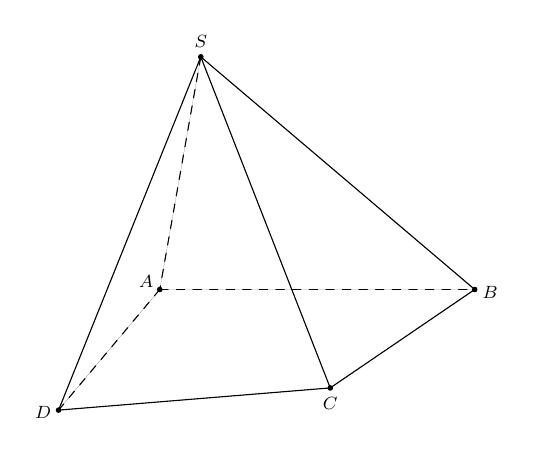
\begin{tikzpicture}[>=stealth,line join=round,line cap=round,font=\footnotesize,scale=1]
				 \tikzset{
					 pics/hinhChopTuGiacthuong/.style n args={5}{
					code={ 
				 \tikzset{
					declare function={a=4; b=2; h=3; goc=-130;  goc2=-30; c=2.5;}
				 }
				 \path
					(0,0) coordinate  (#1)+(0:a) coordinate (#2)+(goc:b) coordinate (#4)+(80:h) coordinate (#5)+(goc2:c) coordinate (#3);
				} 
					}} 
				\path 
					(0,0) pic {hinhChopTuGiacthuong={A}{B}{C}{D}{S}}; 
				\foreach \pointo/\pointt in {S/B,S/C,S/D,B/C,C/D}{ 
					 \draw[fill=black](\pointo)--(\pointt);
				} 
				\foreach  \pointo/\pointt in {S/A,A/B,A/D}{
					\draw[fill=black,dashed](\pointo)--(\pointt); 
				 }
				\foreach \point/\goc in {S/90,A/150,B/-10,C/-90,D/190}{ 
					\draw[fill=black](\point)  circle (.8pt)+(\goc:2mm) node[scale=.8]{$\point$};
				 }
			\end{tikzpicture}
		 }
	} 
\end{ex}

% nguồn: Ok_Toan11_TracNghiem_Lan2
\begin{ex}%[1H4H3-5]%[ma:0c9d0bf9]
	Cho tứ diện $ABCD$. Trên các cạnh $AD$, $BC$ theo thứ tự lấy các  điểm $M$, $N$ sao cho $\dfrac{MA}{AD}=\dfrac{NC}{CB}=\dfrac{1}{3}$. Gọi $(P)$ là mặt phẳng chứa đường thẳng $MN$ và song song với $CD$. Khi đó thiết diện của tứ diện $ABCD$ cắt bởi mặt phẳng $(P)$ là
	 \choice
		{một tam giác} 
		{một hình bình hành} 
		{\True một hình  thang với đáy lớn gấp $2$ lần đáy nhỏ}
		{một hình thang  với đáy lớn gấp $3$ lần đáy nhỏ}
	 \loigiai{
		\begin{center}
			\begin{tikzpicture}[declare function={goc=-45; a=5; b=0.45*a; h=5;}]
					\path 
						(0,0)  coordinate (B)
						(a,0) coordinate  (D)
						(goc:b) coordinate  (C)--+(0,h) coordinate (A)
						($(A)!1/3!(D)$)  coordinate (M)
						($(C)!1/3!(B)$) coordinate (N) 
						($(A)!1/3!(C)$) coordinate (P) 
						($(D)!1/3!(B)$) coordinate  (Q);
					 \draw[dashed] (N)--(Q)--(M)--cycle (B)--(D);
					\draw (N)--(P)--(M) 
						 (A)--(C)
						(A)--(B)--(C)--(D)--cycle; 
					\foreach \x/\goc in {A/90,B/240,D/-60,C/-90,M/30,N/180,P/180,Q/30} 
					\fill  (\x) node[shift={(\goc:7pt)},font=\scriptsize]{$\x$} circle (1pt);
				\end{tikzpicture}
		\end{center}
		 Trong mặt phẳng $(ACD)$, từ $M$ kẻ $MP\parallel CD,\, (P\in AC)$.\\
		Trong mặt phẳng $(BCD)$, từ $M$ kẻ $NQ\parallel CD,\, (Q\in BD)$.\\ 
		Khi đó ta có $MPNQ$ là thiết diện của mặt  phẳng $(P)$ và tứ diện $ABCD$.\\
		Ta có $\heva{&{MP\parallel CD} \\& {MP=\dfrac{1}{3} CD}. 
		 }$ \hfill $(1)$\\
		Mà $\heva{&{NQ  \parallel CD} \\& {NQ=\dfrac{2}{3} CD}.
		}$\hfill $(2)$\\ 
		Từ $(1)$  và $(2)$ ta có $\heva{&{NQ\parallel MP} \\& {MP=\dfrac{1}{2} NQ}.
		 }$\\
		Vậy $MPNQ$  là hình thang có đáy lớn bằng hai lần đáy nhỏ.
	 }
\end{ex}

% nguồn: Ok_Toan11_TracNghiem_Lan2
\begin{ex}%[1H4H3-5]%[ma:ccc084b8]
	Cho hình chóp $S.ABCD$ có đáy $ABCD$ là hình bình hành tâm $O$, $I$ là trung điểm cạnh $SC$. Khẳng  định nào sau đây \textbf{sai}?
	\choice 
		{Đường thẳng $IO$  song song với mặt phẳng $(SAD)$}
		{\True Mặt phẳng $(IBD)$ cắt hình chóp  $S.ABCD$ theo thiết diện là một tứ giác}
		{Đường thẳng  $IO$ song song với mặt phẳng $(SAB)$}
		{Giao tuyến của hai  mặt phẳng $(IBD)$ và $(SAC)$ là $IO$}
	 \loigiai{
		\begin{center}
			\begin{tikzpicture}[declare function={gocx=85; goc=-150; a=4.5; b=a/2; h=4;}]
					\path (0,0) coordinate  (A)--+(gocx:h) coordinate (S)
						 (a,0) coordinate (B)
						(goc:b) coordinate  (D)
						+(a,0)  coordinate (C)
						($(A)!0.5!(C)$) coordinate  (O)
						($(S)!0.5!(C)$) coordinate  (I);
					\draw[dashed]  (S)--(A)
						 (D)--(A)--(B)
						(A)--(C) 
						(B)--(D) 
						 (O)--(I);
					\draw (S)--(D)--(C)--(S)--(B)--(C)--cycle  (D)--(I)--(B);
					\foreach \x/\goc  in {S/90,A/50,B/0,C/-60,D/-180,O/-90,I/30}
					\fill (\x) node[shift={(\goc:7pt)},font=\footnotesize]{$\x$} circle (1pt); 
				\end{tikzpicture}
		\end{center}
		Mặt phẳng $(IBD)$ cắt hình chóp $S.ABCD$ theo thiết diện là tam giác $IBD$. 
	 }
\end{ex}

% nguồn: Ok_Toan11_TracNghiem_Lan2
\begin{ex}%[1H4H3-5]%[ma:5400bbf5]
	Cho hình chóp $S.ABCD$ có đáy $ABCD$ là hình bình  hành. Gọi $M$, $N$, $P$ lần lượt là trung điểm các cạnh $AB$, $AD$, $SC$. Thiết diện hình chóp với mặt phẳng $(MNP)$ là một:
	\choice 
		{tam  giác}
		 {tứ giác}
		{\True  ngũ giác}
		{lục giác} 
	\loigiai{ 
	\immini{ 
		Trong $(ABCD)$ có  $CD$ và $BC$ cắt $MN$ lần lượt tại $I$ và $E$.\\
		Trong $(SBC)$ có $PI$ cắt  $SB$ tại $J$. Trong $(SDC)$: $PE$ cắt $SD$ tại $K$.\\
		Khi đó $(MNP)$ giao với $(ABCD)$, $(SDA)$, $(SBC)$,  $(SAB)$, $(SDC)$ lần lượt theo các giao tuyến $MN$, $NK$, $PJ$, $JM$, $KP$. Nên thiết diện tạo thành là ngũ giác $MNKPJ$.
		}{ 
		\begin{tikzpicture}[>=stealth,line join=round,line cap=round,font=\footnotesize,scale=1]
				 \tikzset{
					pics/hinhChopTuGiac/.style n  args={5}{
					 code={
				\tikzset{ 
					declare function={a=4; b=2;  h=3.5; goc=-150;}
				 }
				 \path
					(0,0) coordinate (#1)+(0:a) coordinate (#2)+(goc:b)  coordinate (#4)+(100:h) coordinate (#5)
					($(#2)+(#4)-(#1)$) coordinate  (#3);
				} 
					}} 
				 \path
					(0,0) pic  {hinhChopTuGiac={A}{B}{C}{D}{S}}
					($(A)!.5!(B)$)  coordinate (M)
					 ($(A)!.5!(D)$) coordinate (N)
					($(S)!.5!(C)$) coordinate (P) 
					(intersection of M--N and C--D)  coordinate (E)
					 (intersection of M--N and B--C) coordinate (I)
					(intersection of E--P  and S--D) coordinate (K)
					(intersection of I--P and  S--B) coordinate (J)
					(intersection of  M--N and S--D) coordinate (M1)
					 (intersection of M--N and S--B) coordinate (M2);
				\foreach  \pointo/\pointt in {S/B,S/D,S/C,C/D,C/B,E/P,I/P,B/I,D/E}{
					\draw[fill=black](\pointo)--(\pointt); 
				 }
				\foreach \pointo/\pointt in {S/A,A/B,A/D,I/E,M/J,N/K,M/P,P/N}{ 
					\draw[fill=black,dashed](\pointo)--(\pointt); 
				} 
				\fill[opacity=.1] (M)--(N)--(K)--(P)--(J)--cycle; 
				\foreach  \point/\goc in {S/90,A/40,B/-90,C/-90,D/90,M/-90,N/-90,I/-90,E/-90,P/70,K/135,J/60}{
					\draw[fill=black](\point) circle (.8pt)+(\goc:2mm) node[scale=.8]{$\point$}; 
				} 
			\end{tikzpicture}
		} 
	 }
\end{ex}

% nguồn: Ok_Toan11_TracNghiem_Lan2
\begin{ex}%[1H4H3-5]%[ma:0e542cf0]
	Cho hìnhchóp $S.ABCD$ có đáy $ABCD$ là hình bình hành. $M$ là một điểm thuộc đoạn $SB$ ($M$ khác $S$ và $B$). Mặtphẳng $(ADM)$  cắt hình chóp $S.ABCD$ theo thiết diện là
	\choice 
		 {Hình bình hành}
		 {Tam giác}
		{Hình chữ nhật} 
		{\True Hình  thang}
	 \loigiai{
		\begin{center}
			\begin{tikzpicture}[declare function={gocx=85; goc=-125; a=4.5; b=0.6*a; h=4;}]
					\path (0,0) coordinate (A)--+(gocx:h) coordinate  (S)
						 (a,0) coordinate (B)
						 (goc:b) coordinate (D)
						+(a,0) coordinate  (C)
						 ($(S)!0.6!(B)$) coordinate (M)
						($(S)!0.6!(C)$) coordinate  (N);
					\draw[dashed]  (A)--(M)--(D)
						 (S)--(A)
						 (D)--(A)--(B);
					\draw (M)--(N)--(D) 
						(S)--(D)--(C)--(S)--(B)--(C)--cycle; 
					 \foreach \x/\goc in {S/90,A/150,B/0,C/-60,D/-180,M/30,N/-30}
					\fill (\x) node[shift={(\goc:7pt)},font=\footnotesize]{$\x$}  circle (1pt);
				\end{tikzpicture}
		\end{center}
		Ta có $M$ là một điểm thuộc đoạn $SB$ với $M$ khác $S$ và $B$.\\ 
		Khi đó  $\heva{&{M\in (ADM)\cap (SBC)} \\& {AD\subset (ADM)} \\& {BC\subset (SBC)} \\& {AD\parallel BC}
		}\Rightarrow (ADM)\cap (SBC)=Mx \parallel BC\parallel AD$.\\ 
		Gọi $N=Mx\cap  SC$ thì $(ADM)$ cắt hình chóp $S.ABCD$ theo thiết diện là tứ giác $AMND$.\\
		Vì $MN\parallel AD$  và $MN$ với $AD$ không bằng nhau nên tứ giác $AMND$ là hình thang.
	 }
\end{ex}

% nguồn: Ok_Toan11_TracNghiem_Lan2
\begin{ex}%[1H4H3-5]%[ma:3621c035]
	Cho hình chóp $S.ABCD$ có  đáy $ABCD$ là hình vuông tại $A$, $B$. Cạnh $SA$ vuông góc với đáy. $M$ là một điểm nằm trên cạnh $AB$. Mặt phẳng $(P)$ đi qua điểm $M$ và song song với $SA$ và $AD$. Khi đó thiết diện của hình chóp $S.ABCD$ cắt bởi mặt phẳng $(P)$ là hình gì?
	\choice 
		 {Hình bình hành}
		{Hình  vuông}
		{\True Hình thang vuông} 
		{Hình chữ  nhật}
	 \loigiai{
		\begin{center}
			\begin{tikzpicture}[scale=1,font=\footnotesize,line join=round,line cap=round,>=stealth]
					\coordinate (A)  at (0,0);
					\coordinate (B) at (2,-2); \coordinate (C) at (4,-2); 
					\coordinate (D) at  (5,0); \coordinate (S) at ($(A)+(0,5)$);
					\coordinate (M) at  ($(A)!0.5!(B)$); \coordinate (Q) at ($(C)!0.5!(D)$);
					\coordinate (N) at ($(S)!0.5!(B)$); \coordinate  (P) at ($(S)!0.5!(C)$);
					\draw (S)--(A)--(B)--(C)--(S)--(B) 
						(C)--(D)--(S) 
						 (M)--(N)--(P)--(Q);
					\draw[dashed]  (A)--(D)
						(P)--(Q)--(M); 
					\pic[draw,angle radius=2mm] {right angle =  B--A--D} pic[draw,angle radius=2mm] {right angle = A--B--C}
						pic[draw,angle radius=2mm] {right angle =  S--A--B};
					 \foreach \i/\g in {S/90,A/180,B/-90,C/-90,D/0,N/180,M/200,P/60,Q/0}{\draw[fill](\i) circle (1pt)
						($(\i)+(\g:3mm)$)  node[scale=1]{$\i$};}
				\end{tikzpicture}
		\end{center}
		 Ta có\\
		$\heva{&(P) \parallel SA\\& M\in (P) \cap  (SAB)} \Rightarrow (P) \cap (SAB)=MN$, $(N\in SB; MN\parallel SA)$.\\
		$\heva{&(P) \parallel AD\\&M\in (P) \cap (ABCD)} \Rightarrow (P) \cap (ABCD)=MQ$,  $(Q\in BC; MQ\parallel AD)$.\\
		$\heva{&(P) \parallel AD\\& N\in (P) \cap ((SBC))} \Rightarrow (P) \cap (SBC)=NP$,  $(P\in SC; NP\parallel BC)$.\\
		Do $SA\perp AB$  nên $MN\perp MQ$.\\
		Vậy thiết diện là hình thang  vuông $MNPQ$.
	} 
\end{ex}

% nguồn: Ok_Toan11_TracNghiem_Lan2
\begin{ex}%[1H4H3-5]%[ma:fcf5fd07]
	Cho hình chóp $S.ABCD$ có đáy  $ABCD$ là hình bình hành. Điểm $M$ thỏa mãn \break $\overrightarrow{MA}=3\overrightarrow{MB}$. Mặt phẳng $(P)$ qua $M$ và song song với hai đường thẳng $SC$, $BD$. Mệnh đề nào sau đây đúng?
	 \choice
		{$(P)$ không cắt hình chóp} 
		{$(P)$ cắt hình chóp theo thiết diện là một tứ giác} 
		{$(P)$ cắt hình chóp theo thiết diện là một tam giác} 
		{\True $(P)$  cắt hình chóp theo thiết diện là một ngũ giác}
	\loigiai{ 
		\begin{center}
			\begin{tikzpicture}[declare function={gocx=85; goc=-135; a=4.5; b=0.6*a; h=4;}]
					 \path (0,0) coordinate (A)--+(gocx:h) coordinate (S)
						(a,0) coordinate  (D)
						(goc:b) coordinate (B) 
						+(a,0)  coordinate (C)
						($(B)!-0.5!(A)$)  coordinate (M)
						($(B)!0.5!(C)$)  coordinate (N)
						($(D)!0.5!(C)$) coordinate  (P)
						 ($(S)!0.5!(B)$) coordinate (F)
						 ($(S)!0.5!(D)$) coordinate (H)
						(intersection of M--F and  S--A) coordinate (G);
					\draw[dashed]  (B)--(D)
						 (N)--(P)
						(F)--(G)--(H) 
						 (F)--(B)--(N)
						(S)--(A) 
						(D)--(A)--(M); 
					\draw  (M)--(N)--(F)--cycle (H)--(P)
						(S)--(D)--(C)--(S)--(F) 
						(N)--(C); 
					\foreach \x/\goc in  {S/90,A/150,B/180,C/-60,D/0,M/180,N/-90,P/0,F/180,H/0,G/30}
					 \fill (\x) node[shift={(\goc:7pt)},font=\footnotesize]{$\x$} circle (1pt);
				\end{tikzpicture}
		\end{center}
		\begin{itemize}
			\item Trong $(ABCD)$, qua $M$ kẻ đường thẳng song song với $BD$ cắt $BC$ và $CD$ lần  lượt tại $N$ và $P$.
			\item Trong $(SBC)$, qua $N$ kẻ đường thẳng  song song với $SC$ cắt $SB$ tại $F$.
			\item Trong $(SCD)$, qua $P$ kẻ đường thẳng song song với $SC$  cắt $SD$ tại $H$.
			\item Trong $(SAB)$, đường thẳng $MF$ cắt $SA$ tại $G$. 
		\end{itemize}
		 Vậy $(P)$ cắt hình chóp theo thiết diện là ngũ giác $NPHGF$.
	} 
\end{ex}

% nguồn: Ok_Toan11_TracNghiem_Lan2
\begin{ex}%[1H4H3-5]%[ma:7b795b08]
	Cho hình  chóp $S.ABCD$ có đáy $ABCD$ là hình thang với đáy lớn là $AB$, điểm $M$ là trung điểm $CD$. Mặt phẳng $(\alpha)$ qua $M$ và song song với cả $SA$, $BC$, cắt hình chóp theo một thiết diện là
	 \choice
		 {hình tam giác}
		{hình bình hành} 
		{hình  thoi}
		{\True hình thang} 
	\loigiai{ 
		\begin{center}
			\begin{tikzpicture}[declare function={goc=-70; gocx=75; a=5; b=0.4*a; c=0.5*a; h=4;}]
					\path  (0,0) coordinate (A)
						(a,0)  coordinate (B)
						(goc:b)  coordinate (D)
						+(c,0)  coordinate (C)
						 (gocx:h) coordinate (S)
						($(D)!0.5!(C)$) coordinate  (M)
						($(M)+(B)-(C)$)  coordinate (H)+(gocx:1cm) coordinate (Ht)
						(intersection of S--B  and H--Ht) coordinate (K)
						($(K)+(C)-(B)$)  coordinate (Kt)
						(intersection of  S--C and K--Kt) coordinate (Q);
					\draw[dashed]  (A)--(B)
						(M)--(H)--(K); 
					\draw  (S)--(A)--(D)
						 (S)--(D)--(C)--(S)--(B)--(C)--cycle (K)--(Q)--(M);
					 \foreach \x/\goc in {S/90,A/-180,B/0,C/-60,D/-100,M/-90,H/40,K/0,Q/180}
					\fill (\x)  node[shift={(\goc:7pt)},font=\footnotesize]{$\x$} circle (1pt);
				\end{tikzpicture}
		\end{center}
		\begin{itemize}
			\item Trong  $(ABCD)$ kẻ đường thẳng qua $M$ song song với $BC$ cắt $AB$ tại $H$.
			\item  Trong $(SAB)$ kẻ đường thẳng qua $H$ song song với $SA$ cắt $SB$ tại $K$.
			\item Trong $(SBC)$ kẻ đường  thẳng qua $K$ song song với $BC$ cắt $SC$ tại $Q$.
		\end{itemize}
		 Thiết diện của hình chóp cắt bởi mặt phẳng $(\alpha)$ hình thang $HKQM$.
	 }
\end{ex}

% nguồn: Ok_Toan11_TracNghiem_Lan2
\begin{ex}%[1H4H3-5]%[ma:e70136d0]
	Cho hình chóp tứ giác $S.ABCD$, có đáy $ABCD$ là hình bình hành. Gọi $H$ là trung điểm của $AC$, $(P)$ là  mặt phẳng qua $H$, song song với $CD$ và $SC$. Thiết diện tạo bởi $(P)$ và hình chóp $S.ABCD$ là hình gì?
	 \choice
		 {Ngũ giác}
		{Hình bình  hành}
		{Tứ giác  không có cặp cạnh đối nào song song}
		 {\True Hình thang}
	 \loigiai{
		\begin{center}
			\begin{tikzpicture}[declare function={gocx=85; goc=-140; a=4.5; b=0.6*a; h=4;}]
					\path (0,0) coordinate (A)--+(gocx:h) coordinate (S) 
						(a,0)  coordinate (B)
						 (goc:b) coordinate (D)
						+(a,0) coordinate (C) 
						($(B)!0.5!(C)$) coordinate  (F)
						 ($(A)!0.5!(D)$) coordinate (E)
						 ($(S)!0.5!(B)$) coordinate (I)
						($(S)!0.5!(A)$) coordinate  (J)
						 ($(A)!0.5!(C)$) coordinate (H);
					\draw[dashed] (A)--(C) 
						 (I)--(J)--(E)--(F)
						(S)--(A) 
						(D)--(A)--(B); 
					 \draw (S)--(D)--(C)--(S)--(B)--(C)--cycle (I)--(F);
					 \foreach \x/\goc in {S/90,A/150,B/0,C/-60,D/-180,F/-30,H/-90,E/180,I/30,J/180}
					\fill (\x) node[shift={(\goc:7pt)},font=\footnotesize]{$\x$}  circle (1pt);
				\end{tikzpicture}
		\end{center}
		$(P)$ là mặt phẳng qua $H$, song song với $CD$ và $SC$ nên $(P)$ cắt $(ABCD)$ theo giao tuyến qua $H$ song song $CD$ cắt $BC$, $AD$ lần lượt tại $F$  và $E$;\\
		$(P)$ cắt $(SBC)$ theo giao tuyến  $FI\parallel SC$,\, ($I\in SB$);\\
		$(P)$ cắt $(SAB)$ theo giao tuyến  $JI\parallel CD$,\, ($J\in SA$).\\
		Khi đó thiết diện tạo bởi $(P)$ và hình chóp $S.ABCD$ là hình thang  $IJEF$ vì $JI\parallel FE$, do cùng song song với $AB$.
	} 
\end{ex}

% nguồn: Ok_Toan11_TracNghiem_Lan2
\begin{ex}%[1H4H3-5]%[ma:d71276dd]
	Cho  hình chóp $S.ABCD$ có đáy $ABCD$ là hình bình hành tâm $O$, $I$ là trung điểm cạnh $SC$. Khẳng định nào sau đây \textbf{sai}?
	\choice 
		{$IO\parallel  (SAB)$}
		{$IO\parallel  (SAD)$}
		{\True Mặt phẳng $(IBD)$ cắt hình chóp $S.ABCD$  theo thiết diện là một tứ giác}
		 {$(IBD)\cap (SAC)=OI$}
	 \loigiai{
		\begin{center}
			\begin{tikzpicture}[declare function={gocx=85; goc=-150; a=4.5; b=a/2; h=4;}]
					 \path (0,0) coordinate (A)--+(gocx:h) coordinate (S)
						(a,0)  coordinate (B)
						(goc:b)  coordinate (D)
						+(a,0) coordinate  (C)
						($(A)!0.5!(C)$) coordinate (O) 
						 ($(S)!0.5!(C)$) coordinate (I);
					\draw[dashed]  (S)--(A)
						 (D)--(A)--(B)
						 (A)--(C)
						 (B)--(D)
						(O)--(I); 
					\draw (S)--(D)--(C)--(S)--(B)--(C)--cycle  (D)--(I)--(B);
					\foreach \x/\goc in {S/90,A/50,B/0,C/-60,D/-180,O/-90,I/30} 
					\fill  (\x) node[shift={(\goc:7pt)},font=\footnotesize]{$\x$} circle (1pt);
				\end{tikzpicture}
		\end{center}
		Trong mặt phẳng $(SAC)$ có $I$, $O$  lần lượt là trung điểm của $SC$, $SA$ nên $IO\parallel SA$.\\
		Suy ra $\heva{&{IO\parallel (SAB)} \\&  {IO \parallel(SAD)}.}$\\
		Hai mặt phẳng $(SAC)$ và $(IBD)$ có hai điểm chung là $O$, $I$ nên giao  tuyến của hai mặt phẳng là $IO$.\\
		Thiết  diện của mặt phẳng $(IBD)$ cắt hình chóp $(S.ABCD)$ là tam giác $IBD$.
	} 
\end{ex}

% nguồn: Ok_Toan11_TracNghiem_Lan2
\begin{ex}%[1H4H3-5]%[ma:8f8e46e2]
	Cho hình chóp $S.ABCD$ có đáy $ABCD$ là hình chữ nhật tâm $O$. Gọi $M$ là trung điểm của $OC$. Mặt phẳng $(\alpha)$ qua $M$  và song song với $SA$ và $BD$. Thiết diện của hình chóp $S.ABCD$ và mặt phẳng $(\alpha)$ là hình gì?
	 \choice
		{\True Hình  tam giác}
		 {Hình bình hành}
		{Hình  chữ nhật}
		{Hình  ngũ giác}
	\loigiai{ 
		\begin{center}
			\begin{tikzpicture}[scale=1,font=\footnotesize,line join=round,line cap=round,>=stealth]
					\coordinate (A)  at (0,0);
					\coordinate (B) at (-2,-2); 
					 \coordinate (D) at (5,0);
					 \coordinate (C) at ($(B)+(D)-(A)$);
					 \coordinate (O) at ($(A)!0.5!(C)$);
					\coordinate (S)  at ($(A)+(1,4)$);
					\coordinate (M) at  ($(O)!0.5!(C)$); \coordinate (E) at ($(B)!0.5!(C)$);
					\coordinate (F)  at ($(D)!0.5!(C)$); \coordinate (K) at ($(S)!3/4!(C)$);
					\draw  (S)--(B)
						(S)--(C)--(D)--(S) 
						(B)--(C) 
						 (E)--(K)--(F);
					 \draw[dashed,thin](A)--(B)
						 (C)--(D)
						(S)--(A)--(D) 
						 (A)--(C)
						(B)--(D) 
						 (K)--(M)
						(E)--(F); 
					\foreach \i/\g in {S/90,A/180,B/-90,C/-90,D/0,O/90,E/-90,F/0,K/70,M/-90}{\draw[fill](\i)  circle (1pt)
						($(\i)+(\g:3mm)$) node[scale=1]{$\i$};} 
				\end{tikzpicture}
		\end{center}
		Qua điểm $M$ kẻ đường thẳng song song với $BD$, cắt $BC$, $CD$ lần lượt tại  $E$, $F$.\\
		Qua điểm $M$ kẻ đường thẳng song song  với $SA$, cắt $SC$ tại $K$.\\
		 Khi đó $(\alpha)\equiv (EFK)$.\\
		Vậy thiết diện là tam giác $EFK$  như hình vẽ.
	 }
\end{ex}

% nguồn: Ok_Toan11_TracNghiem_Lan2
\begin{ex}%[1H4H3-5]%[ma:caac8300]
	Cho tứ diện $ABCD$. Trên các cạnh $AB$, $BC$, $CD$ lần lượt lấy các điểm $P$, $Q$, $R$ sao cho $AP=\dfrac{1}{3}AB$, $BQ=2QC$, $R$ không trùng với $C$, $D$. Gọi $PQRS$ là thiết diện của mặt phẳng $(PQR)$ với  tứ diện $ABCD$. Khi đó $PQRS$ là
	\choice 
		 {hình thang cân}
		{\True hình  thang}
		{một tứ giác không có cặp  cạnh đối nào song song}
		{hình bình  hành}
	 \loigiai{
	 \immini{
		Do $\dfrac{AP}{AB}=\dfrac{CQ}{CB}=\dfrac{1}{3} \Rightarrow PQ  \parallel AC$.\\
		Giao tuyến của mặt phẳng $(PQR)$ và  $(ACD)$ là đường thẳng đi qua $R$ và song song với $AC$, cắt $AD$ tại $S$.\\
		Do  đó $PQRS$ là thiết diện của mặt phẳng $(PQR)$ với tứ diện $ABCD$.\\
		Theo cách dựng thì $PQ \parallel RS$ mà $R$ bất kỳ trên cạnh $CD$ nên  thiết diện là hình thang.
		 }{
		\begin{tikzpicture}[>=stealth,line join=round,line cap=round,font=\footnotesize,scale=1]
				 \tikzset{
					pics/chopTamGiac/.style n args={4}{ 
					code={ 
				 \tikzset{declare function={a=4; b=3; h=3; goc=-20;}}
				\path 
					 (0,0) coordinate (#1)+(0:a) coordinate (#3)+
					(goc:b) coordinate (#2)+(70:h)  coordinate (#4);
				\foreach  \pointo/\pointt in {#4/#1,#1/#2,#2/#3,#3/#4,#4/#2}{
					\draw[fill=black](\pointo)--(\pointt); 
				} 
				\foreach \pointo/\pointt in  {#1/#3}{
					\draw[fill=black,dashed](\pointo)--(\pointt); 
				} 
				} 
					}} 
				 \path
					(0,0)  coordinate (a) pic{chopTamGiac={B}{C}{D}{A}}
					($(A)!1/3!(B)$) coordinate (P) 
					 ($(A)!.5!(D)$) coordinate (S)
					($(B)!2/3!(C)$) coordinate (Q) 
					 ($(C)!.5!(D)$) coordinate (R);
				\foreach \pointo/\pointt in  {P/Q,S/R}{
					\draw[fill=black](\pointo)--(\pointt); 
				 }
				\foreach  \pointo/\pointt in {P/S,Q/R}{
					\draw[fill=black,dashed](\pointo)--(\pointt); 
				 }
				\foreach \point/\goc in {D/-10,A/135,B/190,C/-90,P/130,S/60,R/-45,Q/230}{ 
					\draw[fill=black](\point) circle (.8pt)+(\goc:2mm) node[scale=.8]{$\point$}; 
				} 
			\end{tikzpicture}
		 }
	 }
\end{ex}

% nguồn: Ok_Toan11_TracNghiem_Lan2
\begin{ex}%[1H4H3-5]%[ma:e246eb58]
	Cho tứ diện $ABCD$. Điểm $M$ thuộc đoạn $AC$ ($M$ khác $A$,  $M$ khác $C$). Mặt phẳng $(\alpha)$ đi qua $M$ song song với $AB$ và $AD$. Thiết diện của $(\alpha)$ với tứ diện $ABCD$ là hình gì?
	\choice 
		 {Hình vuông}
		{Hình chữ  nhật}
		{\True  Hình tam giác}
		{Hình bình hành} 
	\loigiai{ 
		\begin{center}
			\begin{tikzpicture}[declare function={goc=-45; a=5; b=0.45*a; h=5;}]
					\path 
						(0,0) coordinate  (B)
						(a,0)  coordinate (D)
						(goc:b) coordinate  (C)--+(0,h) coordinate (A)
						($(A)!1/3!(C)$)  coordinate (M)
						($(B)!1/3!(C)$) coordinate  (N)
						($(D)!1/3!(C)$)  coordinate (P);
					\draw[dashed] (B)--(D) 
						(N)--(P); 
					 \draw (A)--(C)
						(A)--(B)--(C)--(D)--cycle  (N)--(M)--(P);
					\foreach \x/\goc in  {A/90,B/240,D/-60,C/-90,M/30,N/200,P/-30}
					\fill (\x) node[shift={(\goc:7pt)},font=\footnotesize]{$\x$} circle  (1pt);
				\end{tikzpicture}
		\end{center}
		\begin{itemize}
			\item Trong $(ABC)$ kẻ đường thẳng qua $M$ song song  với $AB$ cắt $BC$ tại $N$.
			\item Trong $(ACD)$ kẻ đường thẳng  qua $M$ song song với $AD$ cắt $CD$ tại $P$.
		\end{itemize}
		Do đó thiết diện của $(\alpha)$ với tứ  diện $ABCD$ là hình tam giác $MNP$.
	 }
\end{ex}

% nguồn: Ok_Toan11_TracNghiem_Lan2
\begin{ex}%[1H4H3-5]%[ma:1b8797c8]
	Cho hình chóp  $S.ABCD$ có đáy $ABCD$ là hình bình hành, $M$ là trung điểm $SA$. Gọi $(\alpha)$ là mặt phẳng đi qua $M$, song song với $SC$ và $AD$. Thiết diện của $(\alpha)$ với hình chóp $S.ABCD$ là hình gì?
	 \choice
		{\True Hình thang} 
		{Hình thang  cân}
		 {Hình chữ nhật}
		 {Hình bình hành}
	 \loigiai{
		\begin{center}
			\begin{tikzpicture}[declare function={gocx=85; goc=-140; a=4.5; b=0.6*a; h=4;}]
					\path (0,0) coordinate (A)--+(gocx:h) coordinate (S) 
						(a,0)  coordinate (D)
						 (goc:b) coordinate (B)
						+(a,0) coordinate (C) 
						($(A)!0.5!(B)$) coordinate (Q) 
						($(C)!0.5!(D)$) coordinate  (P)
						($(S)!0.5!(D)$) coordinate (N) 
						($(S)!0.5!(A)$)  coordinate (M);
					\draw[dashed] (N)--(M)--(Q)--(P) 
						(S)--(A) 
						 (D)--(A)--(B);
					\draw  (S)--(D)--(C)--(S)--(B)--(C)--cycle (N)--(P);
					 \foreach \x/\goc in {S/90,A/150,B/180,C/-60,D/0,M/140,N/30,P/-30,Q/160}
					\fill (\x) node[shift={(\goc:7pt)},font=\footnotesize]{$\x$} circle  (1pt);
				\end{tikzpicture}
		\end{center}
		\begin{itemize}
			 \item Trong $(SAD)$, qua $M$ kẻ đường thẳng song song với $AD$ cắt $SD$ tại $N$ .
			\item Trong  $(SCD)$, qua $N$ kẻ đường thẳng song song với $SC$ cắt $CD$ tại $P$.
			\item Trong $(ABCD)$, qua $P$ kẻ đường thẳng song song  với $AD$ cắt $AB$ tại $Q$.
		\end{itemize}
		Vậy $(\alpha)$ cắt hình chóp theo thiết diện là hình  thang $MNPQ$.
	} 
\end{ex}

% nguồn: Ok_Toan11_TracNghiem_Lan2
\begin{ex}%[1H4H3-5]%[ma:db1e1d3c]
	Cho hình chóp $S.ABCD$ có đáy $ABCD$ là hình thang ($AD\parallel BC$, $AD>BC$). Gọi $M$ là trung điểm cạnh $AB$. Mặt phẳng $(P)$ đi qua điểm $M$ và song song với $SA$ và $BC$. Khi đó thiết diện của hình  chóp $S.ABCD$ cắt bởi mặt phẳng $(P)$ là hình gì?
	\choice 
		 {Ngũ giác}
		 {Hình bình hành}
		{Tam  giác}
		{\True Hình  thang}
	 \loigiai{
	\immini{Gọi $N$ là  giao điểm $SB$ và $(P)$.\\
		Suy ra $MN  \parallel SA$\\
		$ \Rightarrow N$ là trung điểm  $SB$.\\
		Gọi $P$, $Q$ là giao điểm  $SC$, $SD$ và $(P)$, tương tự ta có được $P$, $Q$ là trung điểm $SC$, $SD$.\\
		Suy ra $NP \parallel MQ$ nên  tứ giác $MNPQ$ là hình thang.}
		{\begin{tikzpicture}[scale=1,font=\footnotesize,line join=round,line cap=round,>=stealth]
		 \coordinate (A) at (0,0);
		\coordinate (D) at (5,0); 
		\coordinate (C) at (4,-2); 
		\coordinate (B)  at (1,-2);
		\coordinate (S) at ($(A)+(2,5)$); 
		\coordinate (M) at ($(A)!1/2!(B)$); \coordinate  (N) at ($(S)!1/2!(B)$);
		\coordinate (P)  at ($(S)!1/2!(C)$); \coordinate (Q) at ($(C)!1/2!(D)$);
		\draw  (S)--(B)--(A)--(S)--(D)
			 (S)--(C)--(D)--(S)
			(B)--(C) 
			 (M)--(N)--(P)--(Q);
		 \draw[dashed](M)--(Q)
			(A)--(C) 
			(B)--(D)--(A); 
		\foreach \i/\g in {S/90,A/180,B/-90,C/-90,D/0,M/180,N/150,P/30,Q/0}{\draw[fill](\i) circle  (1pt)
			 ($(\i)+(\g:3mm)$) node[scale=1]{$\i$};}
	\end{tikzpicture}
		 }
	} 
\end{ex}

% nguồn: Ok_Toan11_TracNghiem_Lan2
\begin{ex}%[1H4H3-5]%[ma:9c270b57]
	Cho hình chóp $S.ABCD$ có  đáy $ABCD$ là hình bình hành tâm $O$, gọi $I$ là trung điểm cạnh $SC$. Mệnh đề nào sau đây \textbf{sai}?
	\choice 
		{Đường thẳng $IO$  song song với mặt phẳng $(SAD)$}
		{Đường thẳng $IO$ song song  với mặt phẳng $(SAB)$}
		{Mặt  phẳng $(IBD)$ cắt mặt phẳng $(SAC)$ theo giao tuyến $OI$}
		{\True  Mặt phẳng $(IBD)$ cắt hình chóp $S.ABCD$ theo một thiết diện là tứ giác}
	\loigiai{ 
		\begin{center}
			\begin{tikzpicture}[declare function={gocx=85; goc=-150; a=4.5; b=a/2; h=4;}]
					\path (0,0) coordinate (B)--+(gocx:h) coordinate  (S)
						 (a,0) coordinate (C)
						 (goc:b) coordinate (A)
						+(a,0)  coordinate (D)
						 ($(B)!0.5!(D)$) coordinate (O)
						($(S)!0.5!(C)$) coordinate (I); 
					 \draw[dashed] (S)--(B)
						(A)--(B)--(C) 
						(B)--(D) 
						 (C)--(A)
						 (S)--(O)--(I)--(B);
					 \draw (S)--(A)--(D)--(S)--(C)--(D)--cycle (D)--(I);
					 \foreach \x/\goc in {S/90,B/150,C/0,D/-60,A/-180,O/-90,I/30}
					\fill (\x)  node[shift={(\goc:7pt)},font=\footnotesize]{$\x$} circle (1pt);
				\end{tikzpicture}
		\end{center}
		Trong tam giác $SAC$ có $O$ là trung điểm $AC$, $I$ là trung điểm $SC$ nên  $IO\parallel SA$
		$\Rightarrow IO$ song song với hai mặt  phẳng $(SAB)$ và $(SAD)$.\\
		Mặt phẳng  $(IBD)$ cắt $(SAC)$ theo giao tuyến $IO$.\\
		Mặt phẳng $(IBD)$ cắt $(SBC)$ theo giao tuyến $BI$, cắt $(SCD)$ theo giao tuyến $ID$, cắt $(ABCD)$ theo giao tuyến $BD$ suy ra thiết  diện tạo bởi mặt phẳng $(IBD)$ và hình chóp $S.ABCD$ là tam giác $IBD$.
	} 
\end{ex}

% nguồn: Ok_Toan11_TracNghiem_Lan2
\begin{ex}%[1H4H3-5]%[ma:e7c115a2]
	Cho hình chóp $S.ABCD$ có đáy $ABCD$ là hình bình hành. Điểm $M$ thỏa mãn \break $\overrightarrow{MA}=3\overrightarrow{MB}$. Mặt phẳng $(P)$ qua $M$ và song song với $SC$, $BD$. Mệnh đề nào  sau đây đúng?
	\choice 
		{\True $(P)$  cắt hình chóp theo thiết diện là một ngũ giác}
		{$(P)$ cắt  hình chóp theo thiết diện là một tam giác}
		{$(P)$ cắt hình chóp theo  thiết diện là một tứ giác}
		{$(P)$ không cắt hình chóp} 
	\loigiai{ 
		\begin{center}
			\begin{tikzpicture}[declare function={gocx=80; goc=-140; a=4.5; b=a/2; h=4;}]
					 \path (0,0) coordinate (D)--+(gocx:h) coordinate (S)
						(a,0) coordinate  (A)
						(goc:b)  coordinate (C)
						 +(a,0) coordinate (B)
						($(B)!-0.5!(A)$) coordinate  (M)
						($(B)!0.5!(C)$)  coordinate (K)
						 ($(C)!0.25!(A)$) coordinate (N)
						($(D)!0.5!(C)$) coordinate (I) 
						($(D)!0.5!(S)$)  coordinate (P)
						($(B)!0.5!(S)$)  coordinate (Q)
						($(S)!0.25!(A)$) coordinate (R); 
					\draw[dashed] (S)--(D) 
						(C)--(D)--(A) 
						(D)--(B) 
						(A)--(C) 
						(K)--(I)--(P)--(R)--(N); 
					\draw  (S)--(C)--(B)--(S)--(A)--(B)--cycle (B)--(M)--(K)--(Q)--(R);
					\foreach \x/\goc in  {S/90,D/160,A/0,B/-60,C/-180,N/-90,K/-90,M/-30,I/180,P/-30,R/30,Q/0}
					\fill (\x) node[shift={(\goc:7pt)},font=\footnotesize]{$\x$} circle  (1pt);
				\end{tikzpicture}
		\end{center}
		\begin{itemize}
			\item Trong $(ABCD)$  kẻ đường thẳng qua $M$ và song song với $BD$ cắt $BC$, $CD$, $CA$ tại $K$, $N$, $I$.
			\item Trong $(SCD)$ kẻ đường thẳng  qua $N$ và song song với $SC$ cắt $SD$ tại $P$.
			\item Trong $(SCB)$ kẻ đường thẳng qua $K$ và song song với $SC$ cắt  $SB$ tại $Q$.
			\item Trong $(SAC)$ kẻ đường thẳng qua $I$ và song song với  $SC$ cắt $SA$ tại $R$.
		\end{itemize}
		Thiết diện là  ngũ giác $KIPRQ$.
	} 
\end{ex}

% nguồn: Ok_TracNghiemLop11_Lan1
\begin{ex}%[1H4H3-5]%[ma:0df41c08]
	Cho hình chóp $S.ABCD$ có đáy $ABCD$ là hình bình hành.  Gọi $M, N$ lần lượt là trung điểm các cạnh $AB$ và $SD$. Cắt hình chóp bởi mặt phẳng $(CMN)$. Khi đó thiết diện nhận được là
	 \choice
		{một  tam giác}
		{\True một tứ  giác}
		 {một ngũ giác}
		 {một lục giác}
	 \loigiai{
	\immini{Trong mặt phẳng $(ABCD)$ kéo dài $CM$ cắt $AD$ tại $I$. Trong mặt phẳng $(SAD)$ $SA$ cắt $NI$ tại $P$. Vậy thiết diện của  hình chóp cắt bởi mặt phẳng $(CMN)$ là tứ giác $CMPN$.}
		{\begin{tikzpicture}[>=stealth,line join=round,line cap=round,font=\footnotesize,scale=2]
		\draw[scale=2.5] (0,0) coordinate  (A)
			(-120:0.5) coordinate (B)--([turn]120:1) coordinate (C)--(1,0)  coordinate (D)--($(A)+(90:0.6)$) coordinate (S)
			(S)--(C); 
		\draw[dashed,black,scale=2.5] (B)--(A)--(D) 
			(S)--(A); 
		\coordinate (N) at  ($(S)!0.5!(D)$);
		\coordinate (M)  at ($(A)!0.5!(B)$);
		\coordinate  (P) at ($(S)!2/3!(A)$);
		\coordinate (I)  at ($(D)!2!(A)$);
		\path[name path=a](I)--(N); 
		\path[name path=c](I)--(A); 
		 \draw[name path=b](S)--(B);
		\path[name path=d](I)--(M); 
		\path[name intersections={of= a and b}] coordinate (K)  at (intersection-1);
		\path[name intersections={of= c and b}] coordinate (L)  at (intersection-1);
		\path[name intersections={of= d  and b}] coordinate (U) at (intersection-1);
		\draw (I)--(K) 
			(U)--(I)--(L) 
			 (N)--(C);
		 \draw [dashed] (K)--(N)
			(M)--(P) 
			 (L)--(A)--(C)--(U)
			 (B)--(D);
		\path[scale=2.5] pic[angle radius=5,draw=blue,angle eccentricity=1.5] {right  angle = D--A--S};
		\foreach \diem/\vitrin in {N/above,M/below right,I/below,P/below right,S/above,A/above right,B/below left,C/below  right,D/right} \fill (\diem) circle (0.75pt) node[\vitrin]{$\diem$};
	\end{tikzpicture}
		} 
	 }
\end{ex}

% nguồn: Ok_TracNghiemLop11_Lan1
\begin{ex}%[1H4H3-5]%[ma:f9842a39]
	Cắt hình chóp tứ giác bởi mặt phẳng vuông góc với đường cao của hình chóp thiết diện là hình gì? 
	 \choice
		{Một hình bình hành} 
		{Một ngũ  giác}
		{\True Một hình  tứ giác}
		{Một hình  tam giác}
	\loigiai{ 
		\begin{center}
			\begin{tikzpicture}[scale=0.8,line join=round,font=\footnotesize,line cap=round]
					\coordinate (S)  at (1,4);
					\coordinate (A) at (-2,0); 
					\coordinate (B)  at (0,-1.5);
					\coordinate (C)  at (3,-2);
					\coordinate (D) at  (5,0);
					 \coordinate (M) at ($(S)!0.4!(A)$);
					\coordinate  (N) at ($(S)!0.4!(B)$);
					\coordinate (P) at ($(S)!0.4!(C)$); 
					\coordinate  (Q) at ($(S)!0.4!(D)$);
					 \draw (S)--(A)--(B)--(C)--(D)--(S)--(A)
						(B)--(S)--(C) 
						 (M)--(N)--(P)--(Q);
					\draw[dashed]  (A)--(D)
						 (M)--(Q);
					\foreach  \i/\g in {S/90,A/180,B/-90,C/-90,D/0,M/180,N/-140,P/0,Q/0}{\draw[fill](\i) circle (1pt)
						($(\i)+(\g:3mm)$) node{$\i$};} 
				\end{tikzpicture}
		\end{center}
		Mặt phẳng vuông góc với đường cao sẽ  song song với đáy nên cắt hình chóp theo đa giác đồng dạng với đáy.\\
	Vậy thiết diện là hình tứ  giác.}
\end{ex}

% nguồn: Ok_TracNghiemLop11_Lan1
\begin{ex}%[1H4H3-5]%[ma:1d70bd87]
	Cho hình chóp $S.ABCD$ có đáy $ABCD$ ~là hình bình hành. $M$ là một  điểm thuộc đoạn $SB$. Mặt phẳng $\left(ADM\right)$ cắt hình chóp $S.ABCD$ theo thiết diện là
	\choice 
		{\True Hình  thang}
		 {Hình chữ nhật}
		 {Hình bình hành}
		{Tam  giác}
	\loigiai{ 
	\immini{Do $BC\parallel AD$ nên mặt phẳng $\left(ADM\right)$ và  $\left(SBC\right)$ có giao tuyến là đường thẳng $MG$ song song với $BC$. Vậy, thiết diện là hình thang $AMGD$.}
		{\begin{tikzpicture}[font=\footnotesize,scale=.65]
		\def\a{4} 
		\path (0:0)  coordinate (A)
			++(0:\a) coordinate (B) 
			++(-130:.6*\a) coordinate  (C)
			($(A)+(C)-(B)$)  coordinate (D)
			 ($(A)+(80:\a)$) coordinate (S)
			 ($(S)!.55!(B)$) coordinate (M)
			($(S)!.55!(C)$) coordinate (G); 
		\draw[dashed]  (B)--(A)--(D)
			(A)--(S) 
			 (A)--(M);
		\draw  (B)-- (C)--(D)
			(B)--(S) 
			(C)--(S) 
			(D)--(S) 
			(D)--(G)--(M); 
		\foreach  \x/\g in {A/135,B/45,C/-45,D/-135,S/90,M/5,G/-5}
		\fill[black] (\x) circle  (1pt)
			 ($(\g:4mm)+(\x)$) node {$\x$};
	\end{tikzpicture}
		 }
	} 
\end{ex}

% nguồn: Ok_TracNghiemLop11_Lan1
\begin{ex}%[1H4V3-5]%[ma:600360f0]
	Cho hình chóp $S.ABCD$ có $ABCD$ là hình thang cân đáy lớn $AD$. $M,N$ lần lượt là hai trung điểm của $AB$ và $CD$. $(P)$ là mặt phẳng qua $MN$ và cắt mặt bên $(SBC)$ theo  một giao tuyến. Thiết diện của $(P)$ và hình chóp là
	\choice 
		{Hình bình  hành}
		{\True Hình thang} 
		{Hình chữ nhật} 
		 {Hình vuông}
	 \loigiai{
	\immini{Có $MN \parallel BC$  nên $MN \parallel (SBC)$.\\
		Do đó $(P)$ cắt $(SBC)$ theo giao tuyến $PQ$ song song  $MN$.\\
		Vậy thiết diện là hình thang $MNPQ$.} 
		{\begin{tikzpicture}[scale=.7,font=\footnotesize]
		\def\a{5} 
		\def\h{4} 
		 \path (0:0) coordinate (A)
			++(0:\a) coordinate (D) 
			 ($(A)+(-50:.4*\a)$) coordinate (B)
			($(B)+(D)-(A)$)  coordinate (Ct)
			($(B)!1/2!(Ct)$) coordinate (C) 
			($(A)+(60:\h)$) coordinate (S) 
			($(A)!.5!(B)$)  coordinate (M)
			 ($(C)!.5!(D)$) coordinate (N)
			($(S)!.4!(C)$) coordinate (P) 
			($(S)!.4!(B)$) coordinate (Q); 
		\draw[dashed]  (A)--(D)
			(M)--(N); 
		\draw  (A)--(B)--(C)--(D)
			(B)--(S) 
			(C)--(S) 
			 (D)--(S)
			(A)--(S) 
			(M)--(Q)--(P)--(N); 
		\foreach \x/\g in {A/180,B/-135,C/-45,D/0,S/90,M/-135,N/-45,P/45,Q/135} 
		\fill[black] (\x) circle  (1pt)
			 ($(\g:3mm)+(\x)$) node {$\x$};
	\end{tikzpicture}
		} 
	 }
\end{ex}

% nguồn: Ok_TracNghiemLop11_Lan1
\begin{ex}%[1H4V3-5]%[ma:8e17d756]
	Cho hình chóp $S.ABCD$ đáy $ABCD$ là hình thang $(AD\parallel BC)$, gọi $M$ là trung điểm của $AB$. Mặt phẳng $(P)$ đi  qua $M$ và song song với $SA, \; BC$ cắt hình chóp $S.ABCD$ theo thiết diện là hình gì?
	\choice 
		{Ngũ giác} 
		{Hình bình  hành}
		 {Tam giác}
		 {\True Hình thang}
	 \loigiai{
		\begin{center}
			\begin{tikzpicture}[scale=.7,font=\footnotesize]
					 \def\a{6}
					\def\h{4} 
					\path (0:0)  coordinate (A)
						++(0:\a) coordinate  (D)
						($(A)+(-70:.4*\a)$) coordinate (B) 
						($(B)+(D)-(A)$) coordinate (Ct) 
						($(B)!1/3!(Ct)$)  coordinate (C)
						($(A)+(60:\h)$)  coordinate (S)
						($(A)!.5!(B)$)  coordinate (M)
						($(C)!.5!(D)$)  coordinate (N)
						($(S)!.5!(C)$) coordinate  (E)
						 ($(S)!.5!(B)$) coordinate (F);
					\draw[dashed] (A)--(D) 
						 (M)--(N);
					\draw (A)--(B)--(C)--(D) 
						(B)--(S) 
						 (C)--(S)
						 (D)--(S)
						 (A)--(S)
						(M)--(F)--(E)--(N); 
					 \foreach \x/\g in {A/180,B/-135,C/-45,D/0,S/90,M/-135,N/-45,E/45,F/135}
					\fill[black] (\x) circle  (1pt)
						($(\g:3mm)+(\x)$) node {$\x$}; 
				\end{tikzpicture}
		\end{center}
		\begin{itemize}
			\item Trong $(SAB)$, kẻ đường thẳng  qua $M$ song song với $SA$ cắt $SB$ tại $F$.
			\item Trong $(SBC)$, kẻ đường thẳng qua $F$ song song với $BC$  cắt $SC$ tại $E$.
			\item Trong $(ABCD)$, kẻ đường thẳng qua $M$ song song  với $BC$ cắt $CD$ tại $N$.\\
			Suy ra thiết diện của hình chóp $S.ABCD$ cắt bởi mặt phẳng $(P)$ là hình thang $FENM$ vì  có $FE\parallel MN$ (cùng song song với $BC$).
		\end{itemize}
	 }
\end{ex}

% nguồn: Ok_TracNghiemLop11_Lan1
\begin{ex}%[1H4V3-5]%[ma:e86f6b8f]
	Cho tứ diện $ABCD,AB=CD$. Mặt phẳng $(\alpha)$ qua trung điểm  của $AC$ và song song với $AB,CD$ cắt tứ diện đã cho theo thiết diện là
	\choice 
		 {\True Hình thoi}
		{Hình chữ  nhật}
		 {Hình vuông}
		{Hình  tam giác}
	 \loigiai{
		\begin{center}
			\begin{tikzpicture}[font=\footnotesize,scale=.7]
					\def\a{4} 
					\path (0:0) coordinate (B) 
						++(0:\a) coordinate (D) 
						++(-140:.6*\a) coordinate  (C)
						 ($(B)+(70:.8*\a)$) coordinate (A)
						 ($(A)!.5!(C)$) coordinate (M)
						($(B)!.5!(C)$) coordinate (N) 
						($(B)!.5!(D)$) coordinate  (P)
						($(A)!.5!(D)$)  coordinate (Q);
					 \draw[dashed] (B)--(D)
						(N)--(P)--(Q); 
					 \draw (B)--(A)--(D)
						(A)--(C) 
						 (B)--(C)--(D)
						 (N)--(M)--(Q);
					 \foreach \x/\g in {A/90,B/180,C/-45,D/0,M/175,N/-135,P/-45,Q/5}
					\fill[black] (\x) circle (1pt) 
						($(\g:3mm)+(\x)$) node  {$\x$};
				\end{tikzpicture}
		\end{center}
		Gọi $M$ là  trung điểm của $AC$.
		\begin{itemize}
			\item $\heva{&AB\parallel (\alpha)&\\&(ABC)\supset AB\\&M\in (ABC)\cap (\alpha)}\Rightarrow (ABC)\cap  (\alpha)=MN\parallel AB$ với $N$ là trung điểm của $BC$.
			 \item $\heva{&CD\parallel (\alpha)\\&(DBC)\supset CD\\&N\in (DBC)\cap (\alpha)}\Rightarrow (DBC)\cap (\alpha)=NP\parallel CD$ với $P$ là trung điểm của $BD$.
			\item $\heva{&AB\parallel (\alpha)\\&(ABD)\supset AB\\&P\in (ABD)\cap (\alpha)}\Rightarrow (ABD)\cap (\alpha)=PQ\parallel AB$ với $Q$  là trung điểm của $AD$.
			\item Tương  tự có $(ACD)\cap (\alpha)=MQ\parallel CD$.
		\end{itemize}
		Thiết diện của tứ diện cắt bởi $(\alpha)$ là hình  bình hành $MNPQ$ do $MN\parallel PQ,MQ\parallel NP$.\\
		Mặt khác $AB=CD\Rightarrow MN=NP$ (theo tính chất đường trung bình).\\ Vậy $MNPQ$ là  hình thoi.
	 }
\end{ex}

% nguồn: Ok_TracNghiemLop11_Lan1
\begin{ex}%[1H4V3-5]%[ma:9dac1a50]
	Cho tứ diện $ABCD$. $M$ là điểm nằm trong tam  giác $ABC$, mặt phẳng $(\alpha)$ qua $M$ và song song với $AB$ và $CD$. Thiết diện của $ABCD$ cắt bởi mặt phẳng $(\alpha)$ là
	\choice 
		 {Tam giác}
		 {Hình chữ nhật}
		{Hình  vuông}
		{\True  Hình bình hành}
	\loigiai{ 
	\immini{Do $M\in (\alpha), (\alpha)\parallel AB, (\alpha)\parallel CD$ nên\\ $\heva{&(\alpha)\cap (ABC)=IH\parallel AB\\&(\alpha)\cap (ADB)=GF\parallel AB\\&(\alpha)\cap (ADC)=FI\\&(\alpha)\cap (BDC)=GH}$.\\ 
		Mà  $IH=\dfrac{1}{2} AB=HI$ nên $GHIF$ là hình bình hành. }
		{\begin{tikzpicture}[font=\footnotesize,scale=.7]
		\def\a{4} 
		\path (0:0) coordinate (B) 
			++(0:\a) coordinate  (D)
			++(-135:\a/2) coordinate  (C)
			($(B)+(70:\a)$)  coordinate (A)
			($(B)!.45!(C)$) coordinate  (H)
			($(B)!.45!(D)$)  coordinate (G)
			($(C)!.55!(A)$)  coordinate (I)
			($(D)!.55!(A)$) coordinate (F) 
			($(H)!.6!(I)$) coordinate (M); 
		\draw[dashed] (B)--(D) 
			 (H)--(G)--(F);
		\draw  (B)--(A)--(D)
			(A)--(C) 
			 (B)--(C)--(D)
			 (H)--(I)--(F);
		\fill[pattern=north west lines](I)--(F)--(G)--(H)--cycle; 
		 \foreach \x/\g in {A/90,B/180,C/-45,D/0,I/180,F/20,G/-80,H/-90,M/180}
		\fill[black] (\x) circle  (1pt)
			($(\g:3mm)+(\x)$) node  {$\x$};
	\end{tikzpicture}
		} 
	} 
\end{ex}

% nguồn: Ok_TracNghiemLop11_Lan1
\begin{ex}%[1H4V3-5]%[ma:1eced91a]
	Cho tứ diện $ABCD$, điểm $I$ nằm trong tam giác $ABC$, mặt phẳng $(\alpha)$ đi qua $I$ và song song  với $AB,CD$. Thiết diện của tứ diện $ABCD$ và mặt phẳng $(\alpha)$ là
	\choice 
		{hình chữ nhật} 
		{hình vuông} 
		 {\True hình bình hành}
		{tam giác} 
	 \loigiai{
	\immini{\begin{itemize}
		\item Xét trong $(ABC)$ ta có\\ $\heva{&{I\in (\alpha)\cap (ABC)} \\&{(\alpha)\parallel AB}} \Rightarrow (\alpha)\cap (ABC)=ON\parallel AB$, với $I\in ON;O\in  AC;N\in BC$.
		\item Xét trong $(ADC)$ ta có\\ $\heva{&{O\in (\alpha)\cap (ADC)} \\&{(\alpha)\parallel CD}} \Rightarrow (\alpha)\cap (ADC)=OQ\parallel CD$, với $Q\in AD$. 
		\item Xét trong $(BDC)$ ta có\\ $\heva{&{N\in (\alpha)\cap (BDC)} \\&{(\alpha)\parallel CD} 
		}  \Rightarrow (\alpha)\cap (BDC)=NP\parallel \; CD$, với $P\in PD$.\\
		Suy ra $(\alpha)\cap (ABD)=PQ\parallel  AB$.
	\end{itemize}}
	{\begin{tikzpicture}[font=\footnotesize,scale=.7]
		\def\a{4} 
		\path (0:0) coordinate  (B)
			++(0:\a)  coordinate (D)
			++(-135:\a/2) coordinate  (C)
			($(B)+(70:\a)$) coordinate  (A)
			($(B)!.45!(C)$) coordinate (N) 
			($(B)!.45!(D)$) coordinate  (P)
			($(C)!.55!(A)$) coordinate  (O)
			($(D)!.55!(A)$) coordinate (Q) 
			 ($(N)!.6!(O)$) coordinate (I);
		 \draw[dashed] (B)--(D)
			 (N)--(P)--(Q);
		\draw  (B)--(A)--(D)
			 (A)--(C)
			(B)--(C)--(D) 
			 (N)--(O)--(Q);
		\fill[pattern=north  west lines](O)--(N)--(P)--(Q)--cycle;
		\foreach \x/\g in {A/90,B/180,C/-45,D/0,N/-90,P/-60,O/180,Q/45,I/180} 
		\fill[black] (\x) circle (1pt) 
			($(\g:3mm)+(\x)$) node {$\x$}; 
	\end{tikzpicture}
	} 
	Ta có $\heva{&{ON\parallel  QP\parallel AB} \\
	&{OQ\parallel  NP\parallel CD}
	}$  nên thiết diện tạo thành là hình bình hành $ONPQ$.
} 
\end{ex}

% nguồn: Ok_TracNghiemLop11_Lan1
\begin{ex}%[1H4V3-5]%[ma:1cd05737]
	Cho tứ diện $ABCD$. Gọi $H$ là một điểm nằm trong tam giác $ABC$, $(\alpha)$ là mặt phẳng  đi qua $H$ song song với $AB$ và $CD$. Mệnh đề nào sau đây đúng về thiết diện của $(\alpha)$ và tứ diện?
	\choice 
		{Thiết diện  là hình vuông}
		{Thiết diện  là hình thang cân}
		{\True Thiết diện là hình  bình hành}
		{Thiết  diện là hình chữ nhật}
	\loigiai{ 
	\immini{\begin{itemize}
		\item $(ABC)$ cắt $(\alpha)$ theo giao tuyến $MN$ đi qua $H$ và song song với $AB$ ($M\in AC,N\in BC$). 
		\item $(BCD)$ cắt $(\alpha)$ theo giao tuyến $NP\parallel CD$ ($P\in BD$). 
		\item $(ACD)$ cắt $(\alpha)$ theo giao tuyến $MQ\parallel CD$ ($Q\in AD$). 
		\item $(ABD)$ cắt $(\alpha)$ theo giao tuyến $PQ\parallel AB$. 
		\item Có $MQ\parallel NP$ (vì cùng song song  $CD$).
		\item Có $MN\parallel PQ$ (vì  cùng song song $AB$).
	\end{itemize}
	Vậy thiết diện là  hình bình hành $MNPQ$. }
	{\begin{tikzpicture}[font=\footnotesize,scale=.7]
		\def\a{4} 
		\path (0:0)  coordinate (B)
			++(0:\a)  coordinate (D)
			 ++(-135:\a/2) coordinate (C)
			($(B)+(65:\a)$) coordinate (A) 
			($(C)!.5!(A)$) coordinate (M) 
			($(C)!.5!(B)$) coordinate (N) 
			($(B)!.5!(D)$) coordinate  (P)
			($(A)!.5!(D)$)  coordinate (Q);
		 \fill[pattern=dots](M)--(N)--(P)--(Q)--cycle;
		\draw[dashed] (B)--(D) 
			(N)--(P)--(Q); 
		 \draw (B)--(A)--(D)
			 (A)--(C)
			 (B)--(C)--(D)
			(N)--(M)--(Q); 
		\foreach \x/\g in {A/90,B/180,C/-45,D/0,M/180,N/-90,P/-80,Q/45} 
		\fill[black] (\x)  circle (1pt)
			($(\g:3mm)+(\x)$) node {$\x$}; 
	\end{tikzpicture}
	} 
} 
\end{ex}

% nguồn: Ok_TracNghiemLop11_Lan1
\begin{ex}%[1H4V3-5]%[ma:26c03867]
	Cho tứ diện $ABCD$ và điểm $M$ thay đổi trên cạnh $AB$ ($M$ không trùng với các đỉnh). Thiết diện của tứ diện tạo bởi mặt phẳng qua $M$, song song với hai đường thẳng $AC$ và $BD$ luôn  là
	\choice 
		{một  tam giác}
		{một ngũ  giác}
		{một tứ  giác có hai đường chéo vuông góc nhau}
		{\True một tứ giác có hai đường chéo cắt nhau tại trung điểm mỗi đường} 
	 \loigiai{
		\begin{center}
			\begin{tikzpicture}[font=\footnotesize,scale=.7]
					\def\a{4} 
					\path (0:0) coordinate (B) 
						++(0:\a)  coordinate (D)
						++(-120:\a/2)  coordinate (C)
						($(B)+(70:\a)$) coordinate  (A)
						($(B)!.55!(A)$) coordinate (M) 
						($(B)!.55!(C)$) coordinate (N) 
						 ($(D)!.55!(A)$) coordinate (Q)
						($(D)!.55!(C)$) coordinate  (P);
					\draw[dashed] (B)--(D) 
						(M)--(Q) 
						(N)--(P); 
					\draw  (B)--(A)--(D)
						(A)--(C) 
						 (B)--(C)--(D)
						 (M)--(N)
						 (P)--(Q);
					\foreach  \x/\g in {A/90,B/180,C/-45,D/0,M/135,N/-135,P/-45,Q/45}
					\fill[black] (\x)  circle (1pt)
						($(\g:3mm)+(\x)$) node  {$\x$};
				\end{tikzpicture}
		\end{center}
		\begin{itemize}
			\item Từ $M$ dựng đường thẳng song song $AC$, cắt $BC$ tại $N$ thì $MN$ chứa trong mặt phẳng cần  tìm.
			\item Từ $M$ dựng đường thẳng song song $BD$, cắt $AD$ tại $Q$  thì $MQ$ chứa trong mặt phẳng cần tìm. Vậy mặt phẳng qua $M$, song song với hai đường thẳng $AC$ và $BD$ chính là mặt phẳng $\left(MNQ\right)$.
			\item Từ  $N$ dựng đường thẳng song song $BD$, cắt $CD$ tại $P$ thì $NP\subset \left(MNQ\right)$.\\
			Thiết diện là tứ  giác $MNPQ$, tứ giác này có hai cặp cạnh đối song song nên là hình bình hành.
		\end{itemize}
	 }
\end{ex}

% nguồn: Ok_TracNghiemLop11_Lan1
\begin{ex}%[1H4V3-5]%[ma:6af0e4a8]
	Cho hình chóp $S.ABCD$ có đáy là hình bình hành. Gọi $M$, $N$, $P$, $Q$ lần lượt là trung điểm các cạnh $AB$, $CD$, $SD$ và $SA$. Chọn khẳng định {\bf sai} trong các  khẳng định dưới đây.
	\choice 
		{$PN\parallel  (SBC)$}
		 {$MQ\parallel (SBC)$}
		{\True $PQ\parallel (SAD)$} 
		{$MN\parallel  (SAD)$}
	\loigiai{ 
	 \immini{$PQ\subset (SAD)$ nên khẳng định $PQ\parallel (SAD)$ là sai.}
		{\begin{tikzpicture}[font=\footnotesize,scale=.7]
		\def\a{4} 
		\path (0:0) coordinate (A) 
			++(0:\a) coordinate (D) 
			++(-145:.6*\a) coordinate (C) 
			($(A)+(C)-(D)$)  coordinate (B)
			($(A)+(80:\a)$) coordinate  (S)
			($(A)!.5!(B)$) coordinate  (M)
			($(C)!.5!(D)$)  coordinate (N)
			($(S)!.5!(D)$) coordinate (P) 
			($(A)!.5!(S)$) coordinate  (Q);
		 \draw[dashed] (B)--(A)--(D)
			 (A)--(S)
			 (N)--(M)--(Q)--(P);
		\draw  (B)-- (C)--(D)
			 (B)--(S)
			 (C)--(S)
			 (D)--(S)
			 (N)--(P);
		\foreach \x/\g in  {A/135,B/-135,C/-45,D/45,S/90,M/165,N/-45,P/5,Q/135}
		\fill[black] (\x) circle (1pt) 
			 ($(\g:3mm)+(\x)$) node {$\x$};
	\end{tikzpicture}
		 }
	} 
\end{ex}

% nguồn: Ok_TracNghiemLop11_Lan1
\begin{ex}%[1H4V3-5]%[ma:2adf2edf]
	Cho hình chóp $S.ABCD$ có đáy $ABCD$ là hình bình hành. Điểm $M$ thỏa mãn $\overrightarrow{MA}=3\overrightarrow{MB}$. Mặt phẳng $(P)$ qua $M$ và song song với $SC$, $BD$. Mệnh đề nào sau  đây đúng?
	\choice 
		{\True $(P)$ cắt hình  chóp theo thiết diện là một ngũ giác}
		{$(P)$ cắt hình chóp theo  thiết diện là một tam giác}
		{$(P)$ cắt hình chóp theo thiết diện là một tứ giác} 
		{$(P)$ không cắt hình chóp} 
	\loigiai{ 
	\immini{ 
		\begin{itemize}
			 \item Trong $(ABCD)$, kẻ đường thẳng qua $M$ và song song với $BD$ cắt $BC$, $CD$, $CA$ tại $E$, $N$, $I$.
			\item Trong $(SCD)$, kẻ đường thẳng qua $N$ và song song với $SC$ cắt $SD$ tại $P$. 
			\item Trong $(SCB)$, kẻ đường thẳng qua $E$  và song song với $SC$ cắt $SB$ tại $Q$.
			\item Trong $(SAC)$, kẻ đường  thẳng qua $I$ và song song với $SC$ cắt $SA$ tại $R$.
		\end{itemize}
		Thiết diện là ngũ giác  $KNPRQ$. }
		{\begin{tikzpicture}[font=\footnotesize,scale=.7]
		 \def\a{4}
		 \path (0:0) coordinate (D)
			++(0:\a)  coordinate (A)
			 ++(-130:\a/2) coordinate (B)
			($(D)+(B)-(A)$) coordinate  (C)
			($(D)+(95:\a)$)  coordinate (S)
			 ($(A)!1.5!(B)$) coordinate (M)
			 ($(D)!.5!(C)$) coordinate (N)
			($(S)!.5!(D)$)  coordinate (P)
			 ($(S)!.5!(B)$) coordinate (Q)
			($(A)!.75!(S)$)  coordinate (R)
			(intersection  of M--N and B--C) coordinate (E)
			(intersection  of M--N and A--C) coordinate (I);
		\fill[pattern=dots] (N)--(P)--(R)--(Q)--(E)--cycle; 
		\draw[dashed] (C)--(D)--(A)--cycle (B)--(D)--(S) 
			(E)--(N)--(P)--(R) 
			 (I)--(R);
		\draw  (C)--(B)--(A)
			 (B)--(S)
			 (C)--(S)
			 (A)--(S)
			 (E)--(M)--(B)
			(E)--(Q)--(R); 
		\foreach \x/\g in {A/0,B/-45,C/180,D/180,S/90,M/-45,N/135,I/-90,E/-90,R/45,P/180,Q/0} 
		\fill[black] (\x) circle (1pt) 
			 ($(\g:3mm)+(\x)$) node {$\x$};
	\end{tikzpicture}
		} 
	 }
\end{ex}

% nguồn: Ok_TracNghiemLop11_Lan1
\begin{ex}%[1H4V3-5]%[1H4H3-2]%[ma:f053c336]
	 Cho hình chóp tứ giác $S.ABCD$. Gọi $M$ và $N$ lần lượt là trung điểm của $SB$ và $BD$. Khẳng định nào sau đây đúng?
	\choice 
		{$MN\parallel (SAC)$} 
		 {$MN\parallel (SAB)$}
		{$MN\parallel (SBC)$} 
		{\True $MN\parallel  (SAD)$}
	\loigiai{ 
	\immini{Ta có $MN$ là đường trung bình của tam giác  $SBD$.\\
		Suy ra $MN\parallel  SD$.\\
		Mà $SD\subset (SAD)$ nên suy ra  $MN\parallel (SAD)$.}
		{\begin{tikzpicture}
		\def\a{3} 
		\path (0:0) coordinate  (A)
			++(0:\a) coordinate  (D)
			++(-130:.6*\a) coordinate  (C)
			++(172:.5*\a)  coordinate (B)
			($(D)+(105:\a)$) coordinate  (S)
			($(S)!.5!(B)$)  coordinate (M)
			($(B)!.5!(D)$) coordinate  (N);
		\draw[dashed]  (A)--(D)
			(M)--(N) 
			 (B)--(D);
		\draw  (A)--(B)--(C)--(D)
			 (A)--(S)
			(B)--(S) 
			(C)--(S) 
			(D)--(S); 
		\foreach \x/\g in  {A/180,B/-135,C/-45,D/0,S/90,M/170,N/-90}
		\fill[black] (\x)  circle (1pt)
			 ($(\g:3mm)+(\x)$) node {$\x$};
	\end{tikzpicture}
		} 
	} 
\end{ex}

% nguồn: Ok_TracNghiemLop11_Lan1
\begin{ex}%[1H4V3-5]%[ma:88215beb]
	Cho hình chóp $S.ABCD$, đáy  $ABCD$ là hình vuông cạnh bằng $a$. Điểm $M$ trên cạnh $AC$ thỏa mãn $AM=x$, $\left(0< x < a\sqrt{2} \right)$. Mặt phẳng $\left(P\right)$ qua $M$, $\left(P\right)\parallel SA$, $\left(P\right)\parallel BD$ hoặc $\left(P\right)\supset BD$. Giá trị $x$ thỏa mãn điều kiện nào để thiết diện của $\left(P\right)$ và hình chóp $S.ABCD$ là ngũ giác.
	 \choice
		{$0< x <  a\sqrt{2}$}
		{\True $0< x  < \dfrac{a\sqrt{2}}{2}$}
		{$\dfrac{a\sqrt{2}}{2}  \le x < a\sqrt{2}$}
		 {$\dfrac{a}{2} \le x < a\sqrt{2}$}
	 \loigiai{
	\immini{Dựng thiết diện của $\left(P\right)$ và hình chóp  $S.ABCD$.\\
		Ta  có
		\begin{itemize}
			\item Nếu $M$ nằm  giữa $A,C$ thì thiết diện là tứ giác.
			\item Nếu $M$ nằm giữa $O,C$ hoặc trùng với  $O$ thì thiết diện là tam giác.
		\end{itemize}
		nên giá  trị cần tìm của $x$ là $0< x < \dfrac{a\sqrt{2}}{2}$.}
		{\begin{tikzpicture}[font=\footnotesize,scale=.7]
		 \def\a{4}
		\path  (0:0) coordinate (A)
			++(0:\a)  coordinate (D)
			++(-135:.6*\a) coordinate  (C)
			 ($(A)+(C)-(D)$) coordinate (B)
			($(A)+(80:\a)$) coordinate (S) 
			($(A)!.25!(C)$) coordinate (M) 
			($(A)!.5!(B)$) coordinate (P) 
			 ($(A)!.5!(D)$) coordinate (Q)
			($(S)!.25!(C)$) coordinate (N) 
			($(S)!.5!(B)$)  coordinate (E)
			 ($(S)!.5!(D)$) coordinate (F)
			(intersection of A--C and B--D) coordinate  (O);
		\draw[dashed] (B)--(A)--(D) 
			 (A)--(S)
			 (A)--(C)
			 (B)--(D)
			(E)--(P)--(Q)--(F) 
			 (M)--(N);
		 \draw (B)-- (C)--(D)
			(B)--(S) 
			(C)--(S) 
			(D)--(S) 
			 (E)--(N)--(F);
		\foreach  \x/\g in {A/135,B/-135,C/-45,D/45,S/90,O/-90,M/-90}
		\fill[black] (\x)  circle (1pt)
			($(\g:3mm)+(\x)$)  node {$\x$};
	\end{tikzpicture}
		 }
	} 
\end{ex}

% nguồn: Ok_TracNghiemLop11_Lan1
\begin{ex}%[1H4V3-5]%[ma:bf3192fe]
	Cho hình chóp $S.ABCD$ có đáy $ABCD$ là hình thang, $AD\parallel BC$, $AD=3BC$. $M$,  $N$ lần lượt là trung điểm $AB$, $CD$. $G$ là trọng tâm $\triangle SAD$. Mặt phẳng $(GMN)$ cắt hình chóp $S.ABCD$ theo thiết diện là
	 \choice
		{\True  Hình bình hành}
		 {$\triangle GMN$}
		 {$\triangle SMN$}
		 {Ngũ giác}
	 \loigiai{
	\immini{Ta có $(GMN) \parallel AD$ nên giao tuyến của $(GMN)$ và $(SAD)$ là đường thẳng $PQ$ qua $G$ và song song với $AD$.\\ 
		Thiết diện là tứ giác  $MNPQ$ và vì cùng song song với $AD$ nên $MN\parallel PQ$.\tagEX{1}
		\noindent Đặt $BC=a$ khi đó $AD=3a$ nên  $MN=2a$.\\
		Vì $G$ là  trọng tâm $\triangle SAD$ nên $\dfrac{PQ}{AD}=\dfrac{2}{3}$ $\Rightarrow PQ=2a$.\\
		Vậy  $MN=PQ$.\tagEX{2}
		\noindent Từ $(1)$ và  $(2)$ suy ra, $MNPQ$ là hình bình hành. }
		{\begin{tikzpicture}[scale=.7,font=\footnotesize]
		 \def\a{6}
		 \def\h{4}
		\path (0:0) coordinate  (A)
			++(0:\a) coordinate  (D)
			($(A)+(-70:.4*\a)$)  coordinate (B)
			($(B)+(D)-(A)$) coordinate (Ct) 
			($(B)!1/3!(Ct)$)  coordinate (C)
			($(A)+(60:\h)$)  coordinate (S)
			($(A)!.5!(B)$)  coordinate (M)
			($(C)!.5!(D)$)  coordinate (N)
			($(S)!2/3!(A)$) coordinate  (Q)
			 ($(S)!2/3!(D)$) coordinate (P)
			($(A)!.5!(D)$)  coordinate (I)
			 ($(Q)!.5!(P)$) coordinate (G);
		\draw[dashed]  (A)--(D)
			 (M)--(N)
			 (P)--(Q)
			(S)--(I); 
		\draw (A)--(B)--(C)--(D) 
			(B)--(S) 
			 (C)--(S)
			 (D)--(S)
			 (A)--(S)
			 (M)--(Q)
			(P)--(N); 
		 \foreach \x/\g in {A/180,B/-135,C/-45,D/0,S/90,M/-135,N/-45,P/45,Q/135,G/45}
		\fill[black]  (\x) circle (1pt)
			($(\g:3mm)+(\x)$) node  {$\x$};
	\end{tikzpicture}
		} 
	 }
\end{ex}

% nguồn: Ok_TracNghiemLop11_Lan1
\begin{ex}%[1H4V3-5]%[ma:8b47d00e]
	Cho tứ diện $ABCD$. Điểm $M$ thuộc đoạn $AC$ ($M$ khác  $A$, $M$ khác $C$). Mặt phẳng $(\alpha)$ đi qua $M$ song song với $AB$ và $CD$, cắt tứ diện đã cho theo giao tuyến là
	 \choice
		{Hình  vuông}
		{\True Hình bình  hành}
		 {Hình chữ nhật}
		 {Tam giác}
	\loigiai{ 
		\begin{center}
			\begin{tikzpicture}[font=\footnotesize,scale=.7]
					 \def\a{4}
					\path (0:0) coordinate (B) 
						 ++(0:\a) coordinate (D)
						 ++(-140:.6*\a) coordinate (C)
						 ($(B)+(70:.8*\a)$) coordinate (A)
						($(A)!.5!(C)$) coordinate  (M)
						($(B)!.5!(C)$) coordinate  (N)
						($(B)!.5!(D)$)  coordinate (P)
						 ($(A)!.5!(D)$) coordinate (Q);
					 \draw[dashed] (B)--(D)
						 (N)--(P)--(Q);
					\draw  (B)--(A)--(D)
						 (A)--(C)
						 (B)--(C)--(D)
						 (N)--(M)--(Q);
					 \foreach \x/\g in {A/90,B/180,C/-45,D/0,M/175,N/-135,P/-45,Q/5}
					\fill[black]  (\x) circle (1pt)
						($(\g:3mm)+(\x)$) node {$\x$}; 
				\end{tikzpicture}
		\end{center}
		 Ta có
		\begin{itemize}
			\item  $\heva{&AB\parallel(\alpha)\\&AB\subset (ABC)\\&M\in (\alpha)\cap (ABC)}\Rightarrow (ABC)\cap (\alpha)=MN\parallel AB\; (N\in BC)$.
			\item $\heva{&CD\parallel (\alpha)\\&CD\subset (BCD)\\&N\in (\alpha)\cap (BCD)}\Rightarrow (BCD)\cap (\alpha)=NP\parallel CD\; (P\in  BD)$.
			\item $\heva{&AB\parallel (\alpha)\\&AB\subset (ABD)\\ &P\in (\alpha)\cap (ABD)}\Rightarrow (ABD)\cap (\alpha)=PQ\parallel AB\; (Q\in  AD)$.
		\end{itemize}
		Theo cách dựng thì thiết diện $MNPQ$ là hình  bình hành.
	 }
\end{ex}

% nguồn: Ok_TracNghiemLop11_Lan1
\begin{ex}%[1H4V3-5]%[ma:786abbd4]
	Cho hình chóp $S.ABC$ có $E$, $F$ lần lượt là trung điểm cạnh $AB$, $BC$ và điểm $G$ thỏa mãn $\overrightarrow{SG}=\dfrac{1}{2} \overrightarrow{SC}$. Thiết diện của hình chóp $S.ABC$ khi cắt bởi mặt phẳng $(EFG)$ là hình nào dưới  đây?
	 \choice
		{Tam  giác}
		{\True Hình bình hành} 
		{Hình  thang chỉ có một cặp cạnh song song}
		{Hình  thoi}
	 \loigiai{
	 \immini{Ta có
		\begin{itemize}
			\item $EF$ là đường trung bình trong  $\triangle ABC$, suy ra $EF\parallel AC$.\tagEX{1}
			\item $\heva{&(EFG)\cap (SAC)=\{G\}\\ &EF\subset (EFG) \\&AC\subset (SAC)\\&EF\parallel AC}\Rightarrow (EFG)\cap  (SAC)=Gx\parallel FE\parallel AC$.
		\end{itemize}
		Gọi $Gx\cap SA=\left\{H\right\}$, suy ra $H$ là trung điểm $SA$ và $HG\parallel  AC$.\tagEX{2}
		Ta có $\overrightarrow{SG}=\dfrac{1}{2} \overrightarrow{SC}$, suy ra $G$ là trung  điểm của $SC$ và $GF\parallel SB$.\tagEX{3}
		 Ta có $HE$ là đường trung bình trong $\triangle SAB$, suy ra $HE\parallel SB$.\tagEX{4}
		Từ $(1),(2),(3),(4)$  suy ra thiết diện là hình bình hành $FGHE$. }
		{\begin{tikzpicture}[scale=.65]
		 \def\a{3}
		\path (0:0)  coordinate (A)
			 ++(0:\a) coordinate (C)
			++(-120:\a/2) coordinate (B) 
			($(A)+(70:\a)$)  coordinate (S)
			 ($(A)!.5!(B)$) coordinate (E)
			($(C)!.5!(B)$) coordinate (F) 
			($(S)!.5!(C)$)  coordinate (G)
			($(A)!.5!(S)$) coordinate  (H);
		\draw[dashed]  (A)--(C)
			 (H)--(G)
			(E)--(F); 
		\draw (A)--(S)--(C) 
			 (S)--(B)
			 (H)--(E)
			 (F)--(G)
			(A)--(B)--(C); 
		\foreach  \x/\g in {S/90,A/180,B/-45,C/0,E/-135,F/-45,G/30,H/135}
		 \fill[black] (\x) circle (1pt)
			($(\g:3mm)+(\x)$) node {$\x$}; 
	\end{tikzpicture}
		 }
	} 
\end{ex}

% nguồn: Ok_Toan11_TracNghiem_Lan2
\begin{ex}%[1H4C3-5]%[ma:5b920fb2]
	Cho hình chóp tứ giác đều $S.ABCD$ có cạnh đáy bằng $ 10 $. Gọi $M$ là điểm trên $S A$ sao cho $\dfrac{S M}{SA}=\dfrac{2}{3}$. Một mặt phẳng $(\alpha)$ đi qua $M$ song song với  $AB$ và $AD$, cắt hình chóp theo một tứ giác có diện tích là
	\choice 
		 {\True $\dfrac{20}{3}$}
		 {$\dfrac{400}{9}$}
		{$\dfrac{4}{9}$} 
		{$\dfrac{16}{9}$} 
	 \loigiai{
		\begin{center}
			\begin{tikzpicture}[scale=1,font=\footnotesize,line join=round,line cap=round,>=stealth]
					\coordinate (A) at  (0,0);
					\coordinate  (B) at (-2,-3);
					\coordinate (D) at  (7,0);
					\coordinate (C) at ($(B)+(D)-(A)$); 
					\coordinate (S) at  ($(A)+(1,5)$);
					\coordinate  (N) at ($(S)!0.7!(B)$);
					\coordinate  (M) at ($(S)!0.7!(A)$);
					\coordinate (Q) at ($(S)!0.7!(D)$); 
					\coordinate  (P) at ($(S)!0.7!(C)$);
					 \fill[yellow](M)--(N)--(P)--(Q)--cycle;
					\draw  (S)--(B)
						(S)--(C) 
						(S)--(D) 
						(B)--(C)--(D) 
						 (N)--(P)--(Q);
					 \draw[dashed](S)--(A)
						 (A)--(B)
						(A)--(D) 
						 (N)--(M)--(Q);
					\foreach \i/\g  in {S/90,A/45,B/-90,C/-90,D/-90,Q/0,M/45,N/180,P/-120}{\draw[fill=black](\i) circle (1pt)
						($(\i)+(\g:3mm)$)  node[scale=1]{$\i$};}
				\end{tikzpicture}
		\end{center}
		 Ta có $\heva{&AB\parallel(\alpha)\\&AB\subset(SAB)\\&M\in(SAB)\cap(\alpha)}\Rightarrow (\alpha)\cap(SAB)=Mx\parallel AB$.\\
		Ta  lại có $\heva{&AD\parallel(\alpha)\\&AD\subset(SAD)\\&M\in(SAD)\cap(\alpha)}\Rightarrow (\alpha)\cap(SAD)=My\parallel AD$.\\
		Hai tia $Mx$, $My$ cắt $SB$, $SD$ lần  lượt tại $N$, $Q$ và
		\[\heva{&CD\parallel(\alpha)\\&CD\subset(SCD)\\&Q\in(SCD)\cap(\alpha)}\Rightarrow(\alpha)\cap(SCD)=Qz\parallel  CD.\]
		Tia $Qz$ cắt $SC$ tại $P$ nên thiết diện cần  tìm là tứ giác $MNPQ$.\\
		Dễ thấy $\dfrac{2}{3}=\dfrac{SM}{SA}=\dfrac{MN}{AB}=\dfrac{NP}{BC}=\dfrac{PQ}{CD}=\dfrac{QM}{DA}$.\\ $\Rightarrow MN=NP=PQ=QM=\dfrac{20}{3}$.\\ 
		Mặt khác $MN \parallel AB$, $NP \parallel B C$  nên $(MN,NP)=(AB,BC)=90^{\circ}$.\\ Suy ra $MNPQ$ là hình vuông với cạnh $\dfrac{20}{3}$.\\
		Vậy $S_{MNPQ}=\left(\dfrac{20}{3}\right)^{2}=\dfrac{400}{9}$. 
	 }
\end{ex}


%%%%%%%%%%%%%%%% ĐÚNG/SAI %%%%%%%%%%%%%%%%

% nguồn: Ok_dungsai_lop11_Lan1
\begin{ex}%[1H4H3-5]%[ma:a2f7ca4b]
 Cho  hình hộp $ABCD.A'B'C'D'$ có các cạnh $AA'$, $BB'$, $CC'$, $DD'$ song song với nhau. Khi đó
  \choiceTF
  {\True  $(BDA') \parallel(B'D'C')$}
  {\True Đường chéo $AC'$ đi qua trọng tâm $G_1$,  $G_2$ của tam giác $BDA'$ và $B'D'C$}
  {$AG_1=2G_1G_2$} 
  {\True Mặt phẳng  $(A'B'G_2)$ cắt hình hộp $ABCD.A'B'C'D'$ tạo thành một tứ giác là hình bình hành}
 \loigiai{\begin{center}
  \begin{tikzpicture}[line join=round,line cap=round,>=stealth,thick]
    \coordinate (A) at  (-2,-2);
    \coordinate (B) at  (-4,-4);
    \coordinate (C)  at (2,-4);
    \coordinate (D) at  (4,-2);
    \coordinate (A') at  (-2,4);
     \coordinate (B') at (-4,2);
     \coordinate (C') at (2,2);
    \coordinate (D') at (4,4); 
    \coordinate (O') at  (intersection of A'--C' and B'--D');
    \coordinate (O) at (intersection of A--C  and B--D);
    \coordinate  (M) at ($(C')!0.5!(C)$);
    \coordinate (N)  at ($(D')!0.5!(D)$);
    \coordinate (P) at  ($(M)!0.5!(N)$);
     \coordinate (G_1) at (intersection of A'--O and A--C');
    \coordinate  (G_2) at (intersection of C--O' and A--C');
    \draw (A')--(B') 
      (B')--(C')
     (C')--(D') 
      (D')--(A')
      (B')--(D')
     (A')--(C') 
      (B')--(B)
      (C')--(C)
     (D')--(D) 
      (B')--(M)
     (B')--(C) 
     (M)--(N) 
     (D')--(C) 
     (B)--(C) 
      (C)--(D);
     \draw[dashed](A')--(N)
      (A')--(D)
     (A)--(D) 
      (A')--(A)
      (A')--(B)
     (A)--(D) 
      (A)--(B)
      (A)--(C)
     (B)--(D) 
      (A)--(C')
      (A')--(O)
     (A)--(B) 
     (A')--(G_2) 
      (C)--(O')
      (B')--(P);
    \foreach \i in  {A',D',C',O',B'}{\draw (\i) node[scale=0.9,above]{$\i$};}
    \foreach \i  in {G_1,G_2,N,D,C,P}{\draw (\i) node[scale=0.9,right]{$\i$};}
     \foreach \i in {A,B,M}{\draw (\i) node[scale=0.9,left]{$\i$};}
    \foreach \i  in {O}{\draw (\i) node[scale=0.9,below]{$\i$};}
    \foreach \i in  {O',G_1,G_2,O,O',A,B,C,D,A',B',C',D',M,N,P}{\draw[fill=](\i) circle (1pt);}
   \end{tikzpicture}
 \end{center}
 \begin{itemchoice}
  \itemch  \textbf{Đúng}.
  Ta có $BA'D'C$ là hình  bình hành nên $BA' \parallel D'C$.\\
  Ta có $BB'D'D$ là hình bình hành  nên $B'D' \parallel BD$.\\
  Ta có $\heva{&BA'\parallel D'C  \\&
  BD'  \parallel B'D' \\
  &BA',\, BD  \subset (BA'D),\, BA'\cap BD=B\\&
  B'D',\, D'C \subset (B'D'C),\, B'D'\cap  D'C=D'}
  \Rightarrow  (BDA') \parallel (B'D'C)$.
  \itemch \textbf{Đúng}. Trong $(ABCD)$, gọi  $O=AC \cap BD$.
  $\Rightarrow\heva{&O\in AC,\,AC \subset (ACC'A')\\&O \in D,\,  BD \subset (BDA').}$\\
  $\Rightarrow  O \in (ACC'A')\cap (BDA')$.\\
  Mà $A'\in (ACC'A') \cap (BDA')$  nên $A'O=(ACC'A')\cap (BDA')$.\\
  Trong  $(ACC'A')$, gọi $E=A'O \cap AC'$.\\
  Ta  có $\dfrac{{A'E}}{EO}=\dfrac{A'C'}{AO}=2$.\\
  Suy ra $E$ trùng với trọng tâm $G_1$ của tam giác $BDA'\quad(1)$.\\ 
  Trong $(A'B'C'D')$,  gọi $O'=A'C'\cap B'D'$.
  $\Rightarrow \heva{&O'\in  A'C',\, A'C' \subset (ACC'A')\\ &O' \in B'D',\, B'D' \subset (B'D'C)}
  \Rightarrow O' \in (ACC'A')  \cap (B'D'C)$.
  Mà $C \in (ACC'A') \cap (B'D'C)$ nên  $CO=(ACC'A') \cap (B'D'C)$.\\
  Trong  $(ACC'A')$, gọi $F=CO \cap AC'$.\\
  Ta  có $\dfrac{CF}{FO'}=\dfrac{AC}{C'O'}=2$.\\
  Suy ra $F$  trùng với trọng tâm $G_2$ của tam giác $B'D'C.\quad(2)$. \\
  Từ $(1)$ và $(2)$ suy ra $AC'$ qua trọng tâm $G_1$, $G_2$  của tam giác $BDA'$ và $B'D'C$.
  \itemch  \textbf{Sai}.
  Trong $(AA'C'C)$, gọi $I=A'C\cap  AC'$.\\
  \begin{center}
   \begin{tikzpicture}[line join=round,line cap=round,>=stealth,thick]
     \coordinate (A) at (-3,-2); 
     \coordinate (A')  at (-2,1);
     \coordinate  (C') at (3,1);
     \coordinate (C)  at (2,-2);
     \coordinate (O')  at ($(A')!0.5!(C')$);
     \coordinate (O) at ($(A)!0.5!(C)$); 
     \coordinate (G_1) at (intersection  of A'--O and A--C');
     \coordinate (G_2) at (intersection of O'--C and  A--C');
     \coordinate (I) at (intersection  of A'--C and A--C');
     \draw  (A')--(C')
      (C')--(C) 
      (C)--(A) 
      (A)--(A') 
      (A')--(O) 
      (C)--(O') 
      (A')--(C) 
       (A)--(C');
      \foreach \i in {A',O',C'}{\draw (\i) node[scale=0.9,above]{$\i$};}
      \foreach \i in {A,O,C,I}{\draw (\i) node[scale=0.9,below]{$\i$};}
     \foreach \i in {G_1,G_2}{\draw  (\i) node[scale=0.9,below right]{$\i$};}
    \end{tikzpicture}
  \end{center}
  Ta có $G_1$ là trọng tâm của tam giác $A'AC$ nên $$AG_1=\dfrac{2}{3}AI=\dfrac{2}{3}  \cdot \dfrac{1}{2} AC'=\dfrac{1}{3}AC'.$$
  Ta có $G_2$ là trọng tâm của tam giác $A'CC'$ nên $$AG_2=\dfrac{2}{3}C' I=\dfrac{2}{3} \cdot \dfrac{1}{2}AC'=\dfrac{1}{3} AC'.$$ 
  Ta có  $G_1G_2=AC'-AG_1-C'G_2=A C'-\dfrac{1}{3}AC'-\dfrac{1}{3}AC'=\dfrac{1}{3} AC'$.\\
  Từ đó ta có  $AG_1=G_1G_2=G_2C$.\\
  Suy  ra $G_1$, $G_2$ chia đoạn $AC'$ thành ba phần bằng nhau.
   \itemch \textbf{Đúng}.
  Xét tam giác $B'D'C$, gọi $P=B'G_2 \cap  CD'$.\\
  Suy ra $P$  là trung điểm của $CD'$.\\
  Trong $(A'B'G_2)$, vẽ $Px \parallel  AB'$.\\
  Trong $(CC'D'D)$, $Px$ cắt  $CC'$, $DD'$ lần lượt tại $M$ và $N$.\\
  Suy ra $MN\parallel CD$  và $MN=CD$.\\
  Ta có $\heva{&(A'B'G_2)\cap (A'B'C'  D')=A'B' \\
  &(A'B'G_2)  \cap (B'C'CB)=B'M \\
  &(A'B'G_2)\cap (C'D'D)=MN  \\
  &(A'B'G_2)  \cap (AA'D'D)=NA'}.$\\
   $\Rightarrow$ thiết diện của $(A'B'G_2)$ và hình hộp $ABCD.A'B'C'D'$ là tứ giác $A'B'MN$.\\
  Ta có $\heva{&MN \parallel A'B'\\ &MN=A'B'=CD.}$\\ $\Rightarrow$ thiết diện $A'B'MN$  là hình bình hành.
 \end{itemchoice}
 }
\end{ex}

% nguồn: Ok_dungsai_lop11_Lan1
\begin{ex}%[1H4V3-5]%[ma:63ef373d]
 Cho tứ  diện $ABCD$. Giả sử $M$ thuộc đoạn thẳng $BC$. Mặt phẳng $(\alpha)$ qua $M$ song song với $AB$ và $CD$. Khi đó:
 Các mệnh đề  sau đúng hay sai?
 \choiceTF 
  {\True Giao  tuyến của mặt phẳng $(\alpha)$ với mặt phẳng $(ABC)$ là đường thẳng đi qua $M$ và song song với $AB$}
  {\True Giao tuyến của mặt phẳng $(\alpha)$  với mặt phẳng $(BCD)$ là đường thẳng đi qua $M$ và song song với $CD$}
  {\True Giao tuyến của mặt phẳng $(\alpha)$ với mặt phẳng $(ABD)$ là đường thẳng đi qua $N$ và song  song với $AB$}
  {Hình tạo bởi các giao tuyến của mặt  phẳng $(\alpha)$ với các mặt của tứ diện (ta gọi là thiết diện) là hình thang}
  \loigiai{
  \begin{center}
   \begin{tikzpicture}
     \def\a{4} 
      \path (0:0) coordinate (B)
      ++(0:\a)  coordinate (D)
      ++(-135:.65*\a) coordinate (C) 
      ($(B)+(70:\a)$)  coordinate (A)
      ($(C)!.6!(B)$) coordinate (M) 
       ($(C)!.6!(A)$) coordinate (Q)
       ($(B)!.4!(D)$) coordinate (N)
       ($(A)!.4!(D)$) coordinate (P);
      \fill[pattern=north west lines] (M)--(N)--(P)--(Q)--cycle;
     \draw[dashed] (B)--(D) 
       (M)--(N)--(P);
     \draw (B)--(A)--(D) 
       (A)--(C)
      (B)--(C)--(D) 
       (M)--(Q)--(P);
     \foreach \x/\g in {A/90,B/180,C/-45,D/0,M/-90,N/-90,P/45,Q/135} 
     \fill[black] (\x)  circle (1pt)
       ($(\g:3mm)+(\x)$) node {$\x$};
    \end{tikzpicture}
  \end{center}
  \begin{itemchoice}
   \itemch Đúng. Vì $(\alpha)\parallel AB$ nên  giao tuyến của mặt phẳng $(\alpha)$ với mặt phẳng $(ABC)$ là đường thẳng đi qua $M$ và song song với $AB$ và cắt $AC$ tại $Q$.
   \itemch Đúng. Vì $(\alpha)\parallel CD$  nên giao tuyến của mặt phẳng $(\alpha)$ với mặt phẳng $(BCD)$ là đường thẳng đi qua $M$ và song song với $CD$ và cắt $BD$ tại $N$.
    \itemch Đúng. Vì $(\alpha)\parallel AB$ nên giao tuyến của mặt phẳng $(\alpha)$.với mặt phẳng $(ABD)$ là đường thẳng đi qua $N$ và song song với $AB$ và cắt $AD$ tại $P$.
   \itemch  Sai. Ta có $MN\parallel PQ\parallel CD,MQ\parallel PN\parallel AB$.
   Vậy hình tạo bởi các giao tuyến của mặt phẳng $(\alpha)$ với các mặt của tứ diện (ta gọi là thiết  diện) là hình bình hành $MNPQ$.
  \end{itemchoice}
 } 
\end{ex}

% nguồn: Ok_dungsai_lop11_Lan1
\begin{ex}%[1H4V3-5]%[ma:5326af76]
 Cho hình chóp $S.ABCD$ có đáy $ABCD$ là hình  thang $\left(AB\parallel CD\right)$. Gọi $M$, $N$, $P$ lần lượt là trung điểm của $SA$, $BD$ và $AB$.
 \choiceTF 
  {Giao tuyến của mặt phẳng $\left(SAB\right)$  và mặt phẳng $\left(SCD\right)$ là đường thẳng đi qua $S$ và song song với $AC$}
  {\True Giao tuyến của mặt phẳng $\left(MNP\right)$ và mặt phẳng $\left(SAD\right)$ là đường thẳng đi qua $M$ và song  song với $AD$}
  {\True Giao tuyến của  mặt phẳng $\left(DMP\right)$ và mặt phẳng $\left(SBD\right)$ là đường thẳng đi qua $D$ và song song với $MP$}
  {\True Mặt phẳng $\left(\alpha\right)$ qua trung điểm $Q$ của $MN$ và song song với $SA$ và $BD$. Giao tuyến của  $\left(\alpha\right)$ và $\left(SAD\right)$ là đường trung bình của tam giác $SAD$}
 \loigiai{ 
  \begin{center}
   \begin{tikzpicture}[scale=1,font=\footnotesize,line join=round,line cap=round,>=stealth,extended line/.style={shorten >=-#1,shorten <=-#1},
    extended line/.default=3cm]
   \def\ad{3} 
   \def\ab{8} 
   \def\h{4} 
   \def\gocA{-70} 
    \path
     (0,0) coordinate (A)
     (\ab,0) coordinate (B)
     (\gocA:\ad) coordinate (D)
    ($(D)+(3,0)$) coordinate  (C)
     (2,\h) coordinate (S)
     ($(S)!0.5!(A)$) coordinate (M)
    ($(B)!0.5!(D)$) coordinate (N) 
     ($(A)!0.5!(B)$) coordinate (P)
    ($(D)!0.5!(M)$) coordinate (I) 
    ($(B)!0.5!(M)$) coordinate  (J)
    ($(D)!0.5!(A)$) coordinate  (E)
    ($(S)!0.5!(D)$)  coordinate (F)
     (intersection of I--J and M--N) coordinate (Q)
    (intersection of A--C  and B--D) coordinate (O);
   \draw (S)--(A)--(D)--(C)--(B)--(S)--(C)--(D)--(S) 
    (D)--(M) 
    (E)--(F); 
   \draw[dashed] (A)--(C) 
    (B)--(D) 
     (A)--(B)
    (M)--(N)--(P)--cycle  (I)--(J)
     (B)--(M);
   \foreach \p/\q  in {S/90,A/180,B/0,C/-90,D/-90,O/-90,M/180,N/-90,P/90,I/180,J/90,Q/-90,F/0,E/-120}
    \fill[black] (\p) node[shift={(\q:3mm)}]{$\p$} circle (1.0pt);
   \draw [extended line=0.5cm] (S) -- +($(B)-(A)$) node[above]{$ x $};
   \draw [extended line=0.5cm] (M) -- +($(N)-(P)$) node[above]{$ y $};
   \draw [extended line=0.5cm] (D) -- +($(M)-(P)$) node[above]{$ z $};
   \end{tikzpicture}
  \end{center}
  \begin{itemchoice}
   \itemch \textbf{Sai}. $\heva{ 
    &S\in\left(SAB\right)\cap\left(SCD\right)\\
   &AB  \parallel CD\\
    &AB\subset\left(SAB\right),\, CD\subset\left(SCD\right)}
   \Rightarrow\left(SAB\right)\cap\left(SCD\right)=Sx\parallel AB \parallel  CD$.
   \itemch  \textbf{Đúng}. Ta có
   $NP\parallel AD$ (tính chất đường trung bình trong tam  giác $ABD$).\\
   $\heva{ 
   &M\in\left(MNP\right)\cap\left(SAD\right)\\ 
    &NP\parallel AD\\
    &NP\subset\left(MNP\right),\, AD\subset\left(SAD\right)}
   \Rightarrow\left(MNP\right)\cap\left(SAD\right)=My\parallel PN  \parallel AD$.
   \itemch \textbf{Đúng}. Ta  có $\heva{
    &D\in\left(DMP\right)\cap\left(SBD\right)\\
    &MP\parallel SD \\
   &MP\subset\left(DMP\right),\, SD\subset\left(SBD\right)} 
   \Rightarrow\left(DMP\right)\cap\left(SBD\right)=Dz\parallel MP  \parallel SD$.
   \itemch \textbf{Đúng}. Ta có 
   $\heva{&Q\in\left(\alpha\right)\cap\left(MBD\right)\\ 
   &BD\parallel  \left(\alpha\right)\\
    &BD\subset\left(MBD\right)}
   \Rightarrow\left(\alpha\right)\cap\left(MBD\right)=IJ$  \\
    $ IJ $ qua $Q$ song song $BD$ và $I\in DM$, suy ra $I$ là trung điểm $DM$.\\
   Lại có 
   $\heva{ 
    &I\in\left(\alpha\right)\cap\left(SAD\right)\\
   &SA\parallel  \left(\alpha\right)\\
   &SA\subset\left(SAD\right)} 
    \Rightarrow\left(\alpha\right)\cap\left(SAD\right)=EF$
    \\
   $ EF $ qua $I$ song song $SA$ với $E\in AD$, $F\in  SD$.\\
    Vậy $EF$ là đường trung bình của tam giác $SAD$.
  \end{itemchoice}
 } 
\end{ex}

% nguồn: Ok_dungsai_lop11_Lan1
\begin{ex}%[1H4V3-5]%[ma:43b93b9a]
 Cho hình chóp $S.ABCD$ có đáy $ABCD$ là hình bình hành, điểm $M$ di động trên  cạnh $AD$. Một mặt phẳng $(\alpha)$ qua $M$ và song song với hai đường thẳng $CD,SA$, cắt $BC,SC$ và $SD$ lần lượt tại $N,P,Q$. Khi đó:
 Các mệnh đề sau đúng hay sai? 
 \choiceTF 
  {Giao tuyến của mặt phẳng $(\alpha)$ với mặt phẳng $(ABCD)$ là đường thẳng đi qua $M$ và song song  với $AD$}
  {\True Giao tuyến của mặt phẳng $(\alpha)$ với mặt phẳng $(SAD)$ là đường thẳng đi qua $M$ và  song song với $SA$}
  {\True Tứ giác $MNPQ$ là hình thang có  hai đáy là $MN$ và $PQ$}
  {Gọi $I=MQ\cap NP$. Khi đó  $I$ thuộc đường thẳng đi qua $S$ và song song với $AB$}
  \loigiai{
  \begin{center}
   \begin{tikzpicture}
     \def\a{4} 
     \path  (0:0) coordinate (A)
      ++(0:\a)  coordinate (D)
      ++(-130:.65*\a) coordinate (C) 
      ($(A)+(C)-(D)$) coordinate (B) 
      ($(A)+(80:\a)$)  coordinate (S)
      ($(A)!.3!(D)$)  coordinate (M)
      ($(B)!.3!(C)$) coordinate (N) 
      ($(S)!.4!(C)$)  coordinate (P)
      ($(S)!.4!(D)$) coordinate  (Q)
      (intersection  of N--P and M--Q) coordinate (I);
      \draw[dashed] (B)--(A)--(D)
       (A)--(S)--(Q)
      (N)--(M)--(Q); 
     \draw (B)-- (C)--(D) 
       (B)--(S)
       (C)--(S)
       (N)--(I)--(Q)--(D)
       (Q)--(P)
      (S)--(I)--([turn]0:1cm) 
      (I)--(S)--([turn]0:1cm) node[above]{$x$}; 
     \foreach  \x/\g in {A/135,B/-135,C/-45,D/45,S/90,M/-45,N/-90,P/150,Q/0,I/90}
     \fill[black] (\x) circle (1pt) 
       ($(\g:3mm)+(\x)$) node {$\x$};
    \end{tikzpicture}
  \end{center}
   Tứ giác $MNPQ$ là hình gì?\\
  Ta có $\heva{&MN=(\alpha)\cap (ABCD)\\&CD\parallel (\alpha)\\&CD\subset (ABCD)}\Rightarrow (\alpha)\cap  (ABCD)=MN\parallel CD$.\tagEX{1}
  \noindent Tương tự $\heva{&MQ=(\alpha)\cap (SAD)\\&SA\parallel (\alpha)\\&SA\subset (SAD)}\Rightarrow (\alpha)\cap (SAD)=MQ\parallel SA$.\\ $\heva{&PQ=(\alpha)\cap (SCD)\\&CD\parallel (\alpha)\\&CD\subset (SCD)}\Rightarrow  (\alpha)\cap (SCD)=PQ\parallel CD$.\tagEX{2}
  \noindent Từ (1) và (2) suy ra tứ  giác $MNPQ$ là hình thang có hai đáy là $MN$ và $PQ$.\\
  Xét $(SAD)\cap  (SBC)$.
  Ta có $\heva{&S\in (SAD)\cap (SBC)\\&AD\parallel BC\\&AD\subset (SAD),BC\subset (SBC)}\Rightarrow (SAD)\cap (SBC)=Sx$ (với $Sx$ qua $S$ và $Sx\parallel AD\parallel BC$). vì $\heva{&I\in NP,NP\subset (SBC)\\&I\in MQ,MQ\subset (SAD)}\Rightarrow I\in (SAD)\cap  (SBC)$.\\
  Suy  ra $I\in Sx$ (với $Sx$ cố định).\\
   Vậy
  \begin{itemchoice}
   \itemch  Sai.
   \itemch Đúng. 
   \itemch Đúng. 
    \itemch Sai.
  \end{itemchoice}
 } 
\end{ex}

% nguồn: Ok_dungsai_lop11_Lan1
\begin{ex}%[1H4V3-5]%[ma:5901e557]
 Cho hình chóp tứ giác đều $S.ABCD$ có cạnh đáy bằng $2,M$ là một điểm thuộc cạnh $SA$ sao cho $\dfrac{SM}{SA}=\dfrac{2}{3}$. Một mặt phẳng $(\alpha)$  đi qua $M$ song song với $AB$ và $AD$, cắt các mặt của hình chóp theo hình là một tứ giác. Khi đó:
  Các mệnh đề sau đúng hay sai?
  \choiceTF
  {\True Giao tuyến của mặt phẳng $(\alpha)$ với mặt phẳng $(SAB)$ là đường thẳng đi qua  $M$ và song song với $AB$}
  {Giao tuyến của mặt phẳng $(\alpha)$ với mặt phẳng $(SAD)$ là đường thẳng đi qua $M$ và song song với  $SD$}
  {$\dfrac{SM}{SA}=\dfrac{1}{3}$} 
  {\True Mặt phẳng $(\alpha)$ đi qua $M$ song song với $AB$ và $AD$, cắt các mặt của hình chóp theo hình là một tứ giác  có diện tích bằng $\dfrac{16}{9}$}
  \loigiai{
  \begin{center}
   \begin{tikzpicture}[font=\footnotesize,scale=.7]
     \def\a{4} 
     \path (0:0) coordinate  (A)
       ++(0:\a) coordinate (D)
      ++(-140:.6*\a) coordinate  (C)
      ($(A)+(C)-(D)$) coordinate  (B)
      ($(A)+(80:\a)$)  coordinate (S)
      ($(S)!2/3!(A)$)  coordinate (M)
      ($(S)!2/3!(B)$)  coordinate (N)
      ($(S)!2/3!(C)$)  coordinate (P)
      ($(S)!2/3!(D)$)  coordinate (Q);
     \draw[dashed]  (B)--(A)--(D)
      (A)--(S) 
      (N)--(M)--(Q); 
      \draw (B)-- (C)--(D)
       (B)--(S)
       (C)--(S)
      (D)--(S) 
      (N)--(P)--(Q); 
     \foreach \x/\g in  {A/-45,B/-135,C/-45,D/45,S/90,M/45,N/180,P/-45,Q/45}
      \fill[black] (\x) circle (1pt)
      ($(\g:4mm)+(\x)$) node  {$\x$};
    \end{tikzpicture}
  \end{center}
  \begin{itemize}
   \item Vì $\heva{&M\in (SAB)\cap (\alpha)\\&(\alpha)\parallel AB,AB\subset (SAB)}\Rightarrow (SAB)\cap (\alpha)=MN$,  với $MN\parallel AB,N\in SB$.
   \item $\heva{&M\in (SAD.\cap (\alpha)\\&(\alpha)\parallel AD,AD\subset (SAD)}\Rightarrow (SAD)\cap (\alpha)=MQ$, với $MQ\parallel AD,Q\in  SD$.
   \item Vì $BC\parallel AD\parallel  MQ$ và $BC\not \subset (\alpha),MQ\subset (\alpha)$ nên $BC\parallel (\alpha)$.
  \end{itemize}
  Khi đó, ta có $\heva{&N\in (SBC)\cap (\alpha)\\&(\alpha)\parallel BC,BC\subset (SBC)}\Rightarrow  (SBC)\cap (\alpha)=NP$ (với $NP\parallel BC,P\in SC$).\\
  Nối  các đỉnh $M,N,P,Q$ ta được một tứ giác.\\
  Ta có $\heva{&MN\parallel AB\\&MQ\parallel AD\\&NP\parallel BC\\&PQ\parallel CD}$ nên theo định lí Thalès, ta  có
   \[\dfrac{SM}{SA}=\dfrac{SN}{SB}=\dfrac{SP}{SC}=\dfrac{SQ}{SD}=\dfrac{MN}{AB}=\dfrac{NP}{BC}=\dfrac{PQ}{CD}=\dfrac{MQ}{AD}=\dfrac{2}{3}.\]
  Suy ra $MN=NP=PQ=MQ=\dfrac{2}{3} \cdot 2=\dfrac{4}{3}$ (đáy  hình của chóp là hình vuông cạnh $2$).\\
  Dễ thấy $MNPQ$ là một hình  vuông có cạnh bằng $\dfrac{4}{3}$ nên có diện tích bằng $\dfrac{16}{9}$ (đvdt). Vậy
  \begin{itemchoice}
   \itemch  Đúng.
   \itemch  Sai.
    \itemch Sai.
   \itemch  Đúng.
  \end{itemchoice}
  }
\end{ex}

% nguồn: Ok_dungsai_lop11_Lan2
\begin{ex}%[1H4V3-5]%[ma:f9c1dc68]
	Cho hình chóp tứ giác đều $S.ABCD$ có cạnh đáy bằng $2$, $M$ là một điểm thuộc cạnh $SA$ sao cho $\dfrac{SM}{SA}=\dfrac{2}{3}$. Một mặt phẳng $(\alpha)$ đi qua $M$ song song với $AB$ và $AD$, cắt các mặt của hình chóp theo hình là một tứ  giác. Khi đó
	\choiceTF 
		{\True Giao tuyến của mặt phẳng $(\alpha)$ với mặt phẳng $(SAB)$ là  đường thẳng đi qua $M$ và song song với $AB$}
		{Giao tuyến của mặt phẳng $(\alpha)$ với mặt phẳng $(SAD)$ là đường thẳng đi qua  $M$ và song song với $SD$}
		{$\dfrac{SM}{SA}=\dfrac{1}{3}$} 
		{\True Mặt phẳng $(\alpha)$ đi qua $M$ song song với $AB$ và $AD$, cắt các mặt của hình chóp theo  hình là một tứ giác có diện tích bằng $\dfrac{16}{9}$}
	 \loigiai{
		\begin{center}
			\begin{tikzpicture}
					\def\a{4} 
					 \path (0:0) coordinate (A)
						 ++(0:\a) coordinate (D)
						++(-140:.6*\a) coordinate (C) 
						($(A)+(C)-(D)$)  coordinate (B)
						($(A)!0.5!(C)+(0,1.1*\a)$) coordinate  (S)
						($(S)!2/3!(A)$) coordinate (M) 
						($(S)!2/3!(B)$)  coordinate (N)
						 ($(S)!2/3!(C)$) coordinate (P)
						($(S)!2/3!(D)$) coordinate  (Q);
					 \draw[dashed] (B)--(A)--(D)
						(A)--(S) 
						(N)--(M)--(Q); 
					 \draw (B)-- (C)--(D)
						 (B)--(S)
						 (C)--(S)
						(S)--(D) 
						 (N)--(P)--(Q);
					\foreach \x/\g in {A/-90,B/-135,C/-45,D/0,S/90,M/150,N/170,P/70,Q/10} 
					\fill[black]  (\x) circle (1pt)
						($(\g:3mm)+(\x)$)  node {$\x$};
				\end{tikzpicture}
		\end{center}
		\begin{itemchoice}
			 \itemch{\bf Đúng.}\\
			Vì $\heva{&M\in  (SAB)\cap (\alpha)\\&(\alpha)\parallel AB,AB\subset (SAB)}\Rightarrow (SAB)\cap (\alpha)=MN$ với $MN\parallel AB$, $N\in SB$.
			\itemch{\bf Sai.}\\ 
			$\heva{&M\in (SAD)\cap (\alpha)\\&(\alpha)\parallel AD,AD\subset (SAD)}\Rightarrow  (SAD)\cap (\alpha)=MQ$ vơi $MQ\parallel AD$, $Q\in SD$.
			 \itemch{\bf Sai.}\\
			Vì $BC\parallel AD\parallel MQ$ và $BC\not \subset (\alpha)$, $MQ\subset  (\alpha)$ nên $BC\parallel (\alpha)$.\\
			Khi đó,  ta có $\heva{&N\in (SBC)\cap (\alpha)\\&(\alpha)\parallel BC,BC\subset (SBC)}\Rightarrow (SBC)\cap (\alpha)=NP$ (với $NP\parallel BC,P\in SC$).\\
			Nối các đỉnh $M,N,P,Q$  ta được một tứ giác.\\
			Ta có $MN\parallel AB,MQ\parallel AD,NP\parallel BC,PQ\parallel CD$ nên theo định lí Thalès, ta có 
			 \[\dfrac{SM}{SA}=\dfrac{SN}{SB}=\dfrac{SP}{SC}=\dfrac{SQ}{SD}=\dfrac{MN}{AB}=\dfrac{NP}{BC}=\dfrac{PQ}{CD}=\dfrac{MQ}{AD}=\dfrac{2}{3}.
			 \]
			\itemch{\bf  Đúng.}\\
			Ta có $MN=NP=PQ=MQ=\dfrac{2}{3} \cdot  2=\dfrac{4}{3}$ (đáy hình của chóp là hình vuông cạnh $2$).\\
			Dễ thấy $MNPQ$ là một  hình vuông có cạnh bằng $\dfrac{4}{3}$ nên có diện tích bằng $\dfrac{16}{9}$ (đvdt).
		\end{itemchoice}
	} 
\end{ex}

% nguồn: Ok_dungsai_lop11_Lan2
\begin{ex}%[1H4V3-5]%[ma:389963e2]
	Cho hình chóp $S.ABCD$ có tam giác $SAD$ đều. Đáy $ABCD$ là hình thang có $AD\parallel BC$ và $AB=BC=CD=1$, $AD=2$. Gọi $(P)$ là mặt phẳng qua điểm $M$  nằm trên cạnh $AB$ và song song với $\left(SAD\right)$. Đặt $BM=x$ với $\left(0 < x < 1\right)$.
	 \choiceTF
		{\True Thiết diện  của $S.ABCD$ cắt bởi mặt phẳng $(P)$ là một mặt phẳng đi qua $M$ và song song với mặt phẳng $\left(SAD\right)$}
		 {Thiết diện cần tìm là một lục giác đều}
		{Qua $M$ kẻ đường thẳng song song với $AD$ cắt $CD$ tại $N$  thì $MN=1-x$}
		{Để thiết diện  của $S.ABCD$ cắt bởi $(P)$ có diện tích bằng một nửa diện tích tam giác $SAD$ thì giá trị của $x=\dfrac{2}{\sqrt 3}$}
	 \loigiai{
		\begin{center}
			\begin{tikzpicture}[line join=round,line cap=round,line width=.6pt,font=\footnotesize,scale=1]
					\coordinate[label=left:$A$] (A) at  (0,0);
					 \coordinate[label=below left:$B$] (B) at (1.2,-1.6);
					\coordinate[label=below right:$C$] (C)  at (3.2,-1.6);
					\coordinate[label=right:$D$] (D)  at (4.4,0);
					\coordinate[label=above left:$S$] (S) at  (2,4);
					\coordinate[label=below  left:$M$] (M) at ($(A)!2/3!(B)$);
					\coordinate[label=below right:$N$]  (N) at ($(D)!2/3!(C)$);
					\coordinate[label=above right:$P$] (P) at ($(S)!2/3!(C)$); 
					\coordinate[label=above left:$Q$] (Q) at ($(S)!2/3!(B)$); 
					\coordinate[label=above:$I$]  (I) at ($(A)!2/3!(C)$);
					\draw (A)--(B)--(C)--(D)--(S)--cycle  (B)--(S)--(C)
						 (M)--(Q)--(P)--(N);
					 \draw[dashed] (C)--(A)--(D)
						 (M)--(N);
					 \fill (A) circle (1pt)
						(B) circle  (1pt)
						(C) circle  (1pt)
						(D)  circle (1pt)
						(S) circle  (1pt)
						(M) circle  (1pt)
						(N)  circle (1pt)
						(P) circle (1pt) 
						(Q) circle (1pt) 
						(I)  circle (1pt);
				\end{tikzpicture}
		\end{center}
		\begin{itemchoice}
			 \itemch
			Qua $M$ kẻ đường thẳng song song với $AD$ cắt $CD$ tại  $N$.\\
			 Qua $M$ kẻ đường thẳng song song với $SA$ cắt $SB$ tại $Q$.\\
			Qua $Q$ kẻ đường  thẳng song song với $BC$ cắt $SC$ tại $P$.\\
			Suy ra $\left(MNPQ\right)$ là mặt phẳng  qua $M$ và song song với $\left(SAD\right)$.
			 \itemch
			Do đó thiết diện của hình chóp $S.ABCD$ cắt  bởi mặt phẳng $(P)$ là tứ giác $MNPQ$.
			 \itemch
			Bởi vì $MN$ và $PQ$ cùng song song với  $BC$ (hoặc $AD$) nên tứ giác $MNPQ$ là hình thang.\\
			Tam giác $SAD$ đều, cạnh  $AD=2$ nên $SA=SD=2$.\\
			Áp dụng định lí Thales trong các tam giác  $SAB$, $SBC$, $SCD$ ta được
			 $$x=\dfrac{BM}{BA}=\dfrac{MQ}{SA}=\dfrac{BQ}{BS}=\dfrac{CP}{CS}=\dfrac{CN}{CD}=\dfrac{NP}{SD} \text{ và } \dfrac{PQ}{BC}=\dfrac{SQ}{SB}=\dfrac{AM}{AB}=1-x.$$
			Suy ra $MQ=NP=2x$, $CN=x$ và  $PQ=1-x$.\\
			Tiếp tục áp dụng định lí Thales  trong các tam giác $ABC$, $ACD$ ta được\\
			$1-x=\dfrac{AM}{BC}=\dfrac{M\dot I}{BC}$, $x=\dfrac{CN}{CD}=\dfrac{IN}{AD}\Rightarrow MI=1-x$ và $IN=2x  \Rightarrow MN=x+1$.
			\itemch 
			Gọi $H$, $K$ lần lượt là hình chiếu vuông góc của $P$, $Q$ trên $MN$.\\ 
			Ta  có $MK=HN=\dfrac{MN-PQ}{2}=\dfrac{\left(x+1\right)-\left(1-x\right)}{2}=x$.\\
			\begin{center}
				\begin{tikzpicture}[line join=round,line cap=round,line width=.6pt,font=\footnotesize,scale=1]
						\coordinate[label=left:$M$] (M) at (0,0); 
						\coordinate[label=right:$N$] (N) at (6,0); 
						 \coordinate[label=right:$P$] (P) at (4,2);
						\coordinate[label=left:$Q$] (Q)  at (2,2);
						\coordinate[label=below:$K$] (K)  at (2,0);
						\coordinate[label=below:$H$] (H) at  (4,0);
						\draw (M)--(N)--(P)--(Q)--cycle (P)--(H) 
						(Q)--(K); 
						\fill (M) circle (1pt) 
						(N)  circle (1pt)
						(P) circle (1pt) 
						(Q)  circle (1pt)
						(H) circle (1pt) 
						 (K) circle (1pt);
						\newcommand{\gocv}[4][black]{\draw[#1]  ($(#3)!5pt!(#2)$)--($(#3)!2!($($(#3)!5pt!(#2)$)!.5!($(#3)!5pt!(#4)$)$)$)--($(#3)!5pt!(#4)$);}
						 \gocv{Q}{K}{M}
						 \gocv{P}{H}{M}
					\end{tikzpicture}
			\end{center}
			Khi đó, ta có $QK=\sqrt{Q{M^2}-M{K^2}}=\sqrt{4x^2-x^2}=x\sqrt  3 $.\\
			 Suy ra $S_{MNPQ}=\dfrac{\left(PQ+MN\right)\cdot QK}{2}=\dfrac{\left(1-x+1+x\right)\cdot\sqrt 3 x}{2}=\sqrt 3 x$.\\
			Từ giả thiết $S_{MNPQ}=\dfrac{1}{2}\cdot {S_{SBD}}\Leftrightarrow\sqrt  3 x=\dfrac{1}{2}\cdot \dfrac{\left(2x\right)^2\sqrt 3}{4}\Leftrightarrow\sqrt 3 x=\dfrac{x^2\sqrt 3}{2}\Leftrightarrow x=2$.\\
			Vậy  $x=2$.
		\end{itemchoice}
	 }
\end{ex}

% nguồn: Ok_dungsai_lop11_Lan2
\begin{ex}%[1H4V3-5]%[ma:51402597]
	Cho tứ diện $ABCD$ có $G$ là trọng tâm của tam giác $BCD$. Gọi $O$ là trung điểm của đoạn thẳng $AG$. Gọi $S_1$, $S_2$ lần lượt là diện tích thiết diện của  tứ diện cắt bởi mặt phẳng đi qua $O$ đồng thời song song với mặt phẳng $\left(ABC\right)$ và diện tích tam giác $ABC$. Gọi $I$ là trung điểm $BC$. Trong mặt phẳng $\left(AID\right)$ qua $O$ kẻ đường thẳng song song với $AI$ cắt $AD$ tại $P$ và cắt $DI$ tại $J$. Qua $J$ kẻ đường thẳng song song với $MN$, cắt $CD$ tại $N$ và cắt $BD$ tại $M$.
	 \choiceTF
		{Thiết diện cần tìm là một  hình thang}
		{$\dfrac{JD}{ID}=\dfrac{6}{5}$} 
		{\True  $\dfrac{MN}{BC}=\dfrac{5}{6}$}
		 {\True $\dfrac{S_1}{S_2}=\dfrac{25}{26}$}
	 \loigiai{
		\begin{center}
			\begin{tikzpicture}[line join=round,line cap=round,line width=.6pt,font=\footnotesize,scale=1]
					\coordinate[label=left:$B$]  (B) at (0,0);
					\coordinate[label=below left:$C$] (C) at  (2,-2);
					\coordinate[label=right:$D$] (D)  at (6,0);
					\coordinate[label=above left:$A$]  (A) at (4,4);
					\coordinate[label=below:$I$]  (I) at ($(B)!1/2!(C)$);
					\coordinate[label=below:$G$] (G) at ($(D)!2/3!(I)$); 
					 \coordinate[label=right:$O$] (O) at ($(A)!1/2!(G)$);
					\coordinate[label=right:$P$] (P)  at ($(A)!1/6!(D)$);
					\coordinate[label=above left:$M$] (M) at  ($(B)!1/6!(D)$);
					 \coordinate[label=below:$N$] (N) at ($(C)!1/6!(D)$);
					 \coordinate[label=below:$J$] (J) at ($(M)!1/2!(N)$);
					\draw  (A)--(B)--(C)--(D)--cycle (A)--(C)
						(N)--(P); 
					\draw[dashed]  (B)--(D)
						(A)--(G) 
						 (P)--(M)--(N)
						 (D)--(I)
						(P)--(J); 
					\fill  (A) circle (1pt)
						(B) circle  (1pt)
						(C) circle (1pt) 
						 (D) circle (1pt)
						 (M) circle (1pt)
						 (G) circle (1pt)
						 (O) circle (1pt)
						(I) circle (1pt) 
						 (N) circle (1pt)
						(P) circle  (1pt)
						(J) circle (1pt); 
				\end{tikzpicture}
		\end{center}
		\begin{itemchoice}
			 \itemch
			Gọi $I$ là trung điểm $BC$. Trong  mặt phẳng $\left(AID\right)$ qua $O$ kẻ đường thẳng song song với $AI$ cắt $AD$ tại $P$ và cắt $DI$ tại $J$.\\
			Qua $J$ kẻ đường thẳng song song với $MN$, cắt $CD$ tại $N$  và cắt $BD$ tại $M$.\\
			Thiết  diện cần tìm là tam giác $MNP$.
			\itemch 
			Trong tam giác $AIG$ có $OJ\parallel  AI$ hơn nữa $O$ là trung diểm $AG$ nên $J$ là trung điểm $IG$.\\
			Do đó $IJ=\dfrac{1}{2}IG=\dfrac{1}{6}ID\Rightarrow\dfrac{JD}{ID}=\dfrac{5}{6}$. 
			\itemch 
			Suy ra hai tam  giác $MNP$ và $BCA$ đồng dạng theo tỉ số $k=$ $\dfrac{MN}{BC}=\dfrac{JD}{ID}=\dfrac{5}{6}$.
			 \itemch
			Vậy  $\dfrac{S_1}{S_2}=k^2=\dfrac{25}{36}$.
	\end{itemchoice}}
\end{ex}

% nguồn: Ok_dungsai_lop11_Lan2
\begin{ex}%[1H4V3-5]%[ma:c2b763b2]
	Cho hình chóp $S.ABCD$ có đáy $ABCD$ là hình bình hành, mặt bên $SAB$ là tam giác vuông tại $A$, $SA=a\sqrt 3 $, $SB=2a$. Điểm $M$ nằm trên đoạn $AD$ sao cho $AM=2MD$. Gọi $(P)$ là mặt phẳng qua  $M$ và song song với $\left(SAB\right)$.
	 \choiceTF
		{\True Giao tuyến của mặt phẳng $(P)$ với $\left(ABCD\right)$ là $MN$  với $N\in BC$}
		{Thiết diện của hình chóp  cắt bởi mặt phẳng $(P)$ là một hình bình hành}
		{\True Độ dài của  cạnh $AB=a$}
		{Diện tích thiết diện của hình chóp cắt bởi mặt phẳng $(P)$  bằng $\dfrac{5a^2\sqrt 3}{8}$}
	 \loigiai{
		\begin{center}
			\begin{tikzpicture}[line join=round,line cap=round,line width=.6pt,font=\footnotesize,scale=1]
					 \coordinate[label=below left:$B$] (B) at (0,0);
					 \coordinate[label=above left:$A$] (A) at (2,1);
					\coordinate[label=below right:$C$] (C) at (6,0); 
					\coordinate[label=above right:$D$] (D) at ($(C)-(B)+(A)$); 
					\coordinate[label=above left:$S$] (S)  at ($(A)+(90:4)$);
					\coordinate[label=above right:$M$] (M) at ($(A)!2/3!(D)$); 
					 \coordinate[label=below: $N$] (N) at ($(B)!2/3!(C)$);
					\coordinate[label=above:  $P$] (P) at ($(S)!2/3!(C)$);
					\coordinate[label=above:  $Q$] (Q) at ($(S)!2/3!(D)$);
					\draw (B)--(C)--(D)--(S)--cycle  (S)--(C)
						 (N)--(P)--(Q);
					\draw[dashed]  (A)--(D)
						 (S)--(A)--(B)
						 (N)--(M)--(Q);
					 \newcommand{\gocv}[4][black]{\draw[#1] ($(#3)!5pt!(#2)$)--($(#3)!2!($($(#3)!5pt!(#2)$)!.5!($(#3)!5pt!(#4)$)$)$)--($(#3)!5pt!(#4)$);}
					\gocv{S}{A}{B} 
					\fill (A) circle  (1pt)
						(B) circle  (1pt)
						(C) circle  (1pt)
						(D) circle  (1pt)
						(S) circle  (1pt)
						 (M) circle (1pt)
						 (N) circle (1pt)
						 (P) circle (1pt)
						(Q) circle  (1pt);
				\end{tikzpicture}
		\end{center}
		\begin{itemchoice}
			 \itemch
			Ta có $$\heva{&(P)\parallel \left(SAB\right)\\& 
			M\in AD,\,M\in(P)} \Rightarrow  (P)\cap\left(ABCD\right)=MN.$$
			 \itemch
			Tương tự  ta có
			 $(P)\cap\left(SCD\right)=PQ.$\\
			Suy ra $MN\parallel PQ\parallel  AB$.\\
			Lại có $$\heva{&(P) \parallel \left(SAB\right)\\& M\in  AD,\,M\in(P)}
			 \Rightarrow\heva{& (P)\cap\left(SAD\right)=MQ\\
			&(P)\cap\left(SBC\right)=NP.}$$ 
			Suy ra $\heva{& MQ\parallel SA\\&NP\parallel SB.}$\\ 
			Mà tam giác $SAB$  vuông tại $A$ nên $SA\perp AB\Rightarrow MN\perp MQ$.
			Từ đó suy ra $(P)$ cắt hình chóp theo thiết diện là hình thang vuông  tại $M$ và $Q$.
			\itemch 
			Mặt khác $MQ\parallel SA$  $\Rightarrow\dfrac{MQ}{SA}=\dfrac{DM}{DA}=\dfrac{DQ}{DS} \Rightarrow MQ=\dfrac{1}{3}SA$ và $\dfrac{DQ}{DS}=\dfrac{1}{3}$.\\
			$PQ\parallel CD  \Rightarrow\dfrac{PQ}{CD}=\dfrac{SQ}{SD} \Rightarrow PQ=\dfrac{2}{3}AB$, với $AB=\sqrt{S{B^2}-S{A^2}}=a$.
			 \itemch
			 Khi đó $S_{MNPQ}=\dfrac{1}{2}MQ\cdot \left(PQ+MN\right)=\dfrac{1}{2}\dfrac{SA}{3}\cdot \left(\dfrac{2AB}{3}+AB\right)=\dfrac{5a^2\sqrt 3}{18}$.
	\end{itemchoice}}
\end{ex}

% nguồn: Ok_dungsai_lop11_Lan2
\begin{ex}%[1H4V3-5]%[ma:76bd9cf2]
	Cho tứ diện $ABCD$ có tất cả các cạnh đều bằng nhau. Gọi $I$ là trung điểm đoạn $CD$ và $M$ là điểm nằm trên đoạn $BC$ ($M$ khác  $B$ và $C$). Gọi $\left(\alpha\right)$ là mặt phẳng qua $M$ và song song với mặt phẳng $\left(ABI\right)$.
	 \choiceTF
		{\True Giao tuyến của $\left(\alpha\right)$ và  mặt phẳng $\left(BCD\right)$ là $MP$ với $P\in CD$}
		{Giao tuyến của $\left(\alpha\right)$  và mặt phẳng $\left(ACD\right)$ là $MQ$ với $Q\in AC$}
		 {$PQ=\left(\alpha\right)\cap\left(ABC\right)$}
		{\True Thiết  diện của tứ diện $ABCD$ khi cắt bởi $\left(\alpha\right)$ là một tam giác cân}
	\loigiai{ 
		\begin{center}
			\begin{tikzpicture}[line join=round,line cap=round,line width=.6pt,font=\footnotesize,scale=1]
					\coordinate[label=left:$B$]  (B) at (0,0);
					\coordinate[label=below  left:$C$] (C) at (2,-2);
					 \coordinate[label=right:$D$] (D) at (6,0);
					 \coordinate[label=above left:$A$] (A) at (4,4);
					 \coordinate[label=below:$I$] (I) at ($(C)!1/2!(D)$);
					 \coordinate[label=below:$P$] (P) at ($(C)!1/2!(I)$);
					 \coordinate[label=below:$M$] (M) at ($(B)!1/2!(C)$);
					\coordinate[label=above  left:$Q$] (Q) at ($(A)!1/2!(C)$);
					\draw (A)--(B)--(C)--(D)--cycle  (A)--(C)
						 (M)--(Q)--(P);
					\draw (A)--(I); 
					\draw[dashed] (B)--(D) 
						 (M)--(P)
						(B)--(I); 
					\fill  (A) circle (1pt)
						(B)  circle (1pt)
						(C) circle (1pt) 
						 (D) circle (1pt)
						(M)  circle (1pt)
						(P)  circle (1pt)
						(Q) circle  (1pt)
						(I)  circle (1pt);
				\end{tikzpicture}
		\end{center}
		\begin{itemchoice}
			\itemch 
			Theo giả thiết ta có $IA=IB$ suy ra $\triangle AIB$ cân tại  $I$.\\
			Do $\left(\alpha\right)$ là mặt phẳng qua $M$ và  song song với mặt phẳng $\left(ABI\right)$ nên:
			Trong $\left(BCD\right)$ kẻ $MP\parallel BI$, $P\in CD$ suy  ra $MP=\left(\alpha\right)\cap\left(BCD\right)$.
			 \itemch
			Trong  $\left(ACD\right)$ kẻ $PQ\parallel AI$, $Q\in AC$ suy ra $PQ=\left(\alpha\right)\cap\left(ACD\right)$.
			\itemch 
			Khi  đó $MQ=\left(\alpha\right)\cap\left(ABC\right)$.
			\itemch 
			Thiết diện diện của  tứ diện $ABCD$ khi cắt bởi $\left(\alpha\right)$ là $\triangle MPQ$ thì theo cách dựng ta suy ra $\triangle MPQ$ đồng dạng với $\triangle BIA$ suy ra $\triangle MPQ$ cân tại $P$.
	\end{itemchoice}}
\end{ex}


%%%%%%%%%%%%%%%% TRẢ LỜI NGẮN %%%%%%%%%%%%%%%%

% nguồn: Ok_TraLoiNgan_Lop11_Lan1
\begin{ex}%[1H4V3-5]%[ma:cca9a681]
	Cho hình chóp $S.ABCD$ có đáy $ABCD$ là hình bình hành và một điểm $M$ nằm trên cạnh $AD$ (giữa $A$ và $D$) sao cho $AD = 3MD$. Một mặt phẳng $(\alpha)$ đi qua $M$, song song với $CD$ và $SA$, cắt $BC$, $SC$, $SD$ lần lượt tại $N$, $P$, $Q$. Với cạnh $CD  = 9{,}3$ (cm) thì độ dài đoạn $PQ$ là bao nhiêu?
	\begin{center}
		\begin{tikzpicture}[scale=0.5,font=\footnotesize,line join=round,line cap=round,>=stealth]
				\path 
					 (0,0) coordinate (A)
					 ++(-140:3) coordinate (B)
					++(0:8)  coordinate (C)
					 ($(A)+(C)-(B)$) coordinate (D)
					($(A)+(1,6)$)  coordinate (S)
					($(D)!1/3!(A)$) coordinate (M) 
					($(C)!1/3!(B)$) coordinate  (N)
					($(C)!1/3!(S)$)  coordinate (P)
					 ($(D)!1/3!(S)$) coordinate (Q);
				\foreach \i in{B,C,D}{\draw (S)--(\i);}; 
				\draw (B)--(C)--(D) 
					 (N)--(P)--(Q);
				\draw[dashed]  (S)--(A)--(B)
					(A)--(D) 
					 (N)--(M)--(Q);
				\foreach  \i/\g in {A/-90,B/-90,C/-90,D/-90,S/90,M/-60,N/-90,P/180,Q/60}
				\fill[black] (\i) circle (1pt)+(\g:3mm)  node[scale=1]{$\i$};
			\end{tikzpicture}
	\end{center}
	 \shortans{6,2}
	\loigiai{ 
		\begin{center}
			\begin{tikzpicture}[scale=0.5,font=\footnotesize,line join=round,line cap=round,>=stealth]
					\path 
						(0,0)  coordinate (A)
						++(-140:3) coordinate  (B)
						++(0:8) coordinate  (C)
						($(A)+(C)-(B)$) coordinate (D) 
						 ($(A)+(1,6)$) coordinate (S)
						($(D)!1/3!(A)$) coordinate (M) 
						($(C)!1/3!(B)$)  coordinate (N)
						($(C)!1/3!(S)$)  coordinate (P)
						($(D)!1/3!(S)$) coordinate  (Q);
					\foreach  \i in{B,C,D}{\draw (S)--(\i);};
					\draw  (B)--(C)--(D)
						 (N)--(P)--(Q);
					\draw[dashed] (S)--(A)--(B) 
						(A)--(D) 
						(N)--(M)--(Q); 
					\foreach  \i/\g in {A/-90,B/-90,C/-90,D/-90,S/90,M/-60,N/-90,P/180,Q/60}
					 \fill[black] (\i) circle (1pt)+(\g:3mm) node[scale=1]{$\i$};
				\end{tikzpicture}
		\end{center}
		Ta có $MN$, $CD$, $PQ$ là ba giao tuyến của ba mặt phẳng $(ABCD)$, $(MNPQ)$, $(SCD)$.\\ Theo Định lý ba đường giao tuyến ta suy ra  $MN \parallel CD \parallel PQ$.\\
		Theo tính chất song song, $SA \parallel (\alpha)$ nên $SA  \parallel MQ$, với $MQ$ là giao tuyến của $(\alpha)$ với $(SAD)$.\\
		Theo  Định lý Thales trong $\triangle SAD$ và $\triangle SCD$\\
		$\dfrac{PQ}{CD} = \dfrac{SQ}{SD} = \dfrac{AM}{AD} =  \dfrac{2}{3} \Rightarrow PQ = \dfrac{2}{3} \cdot 9{,}3 = 6{,}2$.
	 }
\end{ex}

% nguồn: Ok_TraLoiNgan_Lop11_Lan1
\begin{ex}%[1H4V3-5]%[ma:d150f8a0]
	Cho tứ diện $ABCD$ có $AB$ vuông góc với $CD$, $AB=4,^{} CD=6$. $M$ là điểm thuộc cạnh $BC$ sao cho $MC=2BM$. Mặt phẳng $\left(P\right)$ đi  qua $M$ song song với $AB$ và $CD$. Tính diện tích thiết diện của $\left(P\right)$ với tứ diện (làm tròn kết quả đến hàng phần trăm).
	 \shortans{5,33}
	\loigiai{ 
		\begin{center}
			\begin{tikzpicture}
					 \def\a{4}
					 \path (0:0) coordinate (B)
						++(0:\a) coordinate  (D)
						++(-148:.7*\a) coordinate (C) 
						 ($(B)+(70:\a)$) coordinate (A)
						($(C)!.5!(B)$) coordinate (M) 
						($(C)!.5!(A)$)  coordinate (N)
						 ($(D)!.5!(A)$) coordinate (P)
						 ($(D)!.5!(B)$) coordinate (Q);
					\draw[dashed]  (B)--(D)
						 (M)--(Q)--(P);
					\draw  (B)--(A)--(D)
						(A)--(C) 
						 (B)--(C)--(D)
						(M)--(N)--(P); 
					\foreach \x/\g  in {A/90,B/180,C/-45,D/0,M/-135,N/135,P/20,Q/-45}
					 \fill[black] (\x) circle (1pt)
						($(\g:3mm)+(\x)$) node {$\x$}; 
				\end{tikzpicture}
		\end{center}
		Ta có  $\left(AB,CD\right)=\left(MN,MQ\right)=\widehat{NMQ}=90^\circ$.\\
		Suy ra  thiết diện $MNPQ$ là hình chữ nhật.\\
		 Lại có
		\begin{itemize}
			\item $\triangle CMN\backsim  \triangle CBA\Rightarrow \dfrac{CM}{CB}=\dfrac{MN}{AB}=\dfrac{1}{3} \Rightarrow MN=\dfrac{4}{3}$.
			\item $\triangle ANP\backsim \triangle  ACD\Rightarrow \dfrac{AN}{AC}=\dfrac{NP}{CD}=\dfrac{2}{3} \Rightarrow MP=4$.
		\end{itemize}
		Suy ra  $S_{MNPQ}=MN\cdot NP=\dfrac{16}{3}\approx 5{,}33$.
	} 
\end{ex}

% nguồn: Ok_TraLoiNgan_Lop11_Lan1
\begin{ex}%[1H4V3-5]%[ma:ae2eac0e]
	Cho hình chóp $S.ABCD$ có đáy $ABCD$ là hình bình hành. Gọi $C'$ là điểm trên cạnh $SC$ sao cho $\dfrac{C'S}{C'C}=\dfrac{1}{2}$, $M$ là điểm trên cạnh $SA$. Mặt phẳng $\left(P\right)$ qua $C'M$ và song song với $BC$. Khi $\left(P\right)$ cắt hình chóp theo thiết diện là hình bình hành thì tỉ  số $\dfrac{MA}{MS}$ bằng bao nhiêu.
	\shortans{2} 
	 \loigiai{
		\begin{center}
			\begin{tikzpicture}[scale=.7,font=\footnotesize]
					 \def\a{4}
					\path (0:0) coordinate  (A)
						 ++(0:\a) coordinate (D)
						++(-130:.6*\a) coordinate  (C)
						($(A)+(C)-(D)$)  coordinate (B)
						($(A)+(100:\a)$)  coordinate (S)
						($(S)!1/3!(C)$) coordinate (C') 
						($(S)!1/3!(A)$)  coordinate (M)
						 ($(S)!1/3!(B)$) coordinate (N)
						($(S)!1/3!(D)$) coordinate (P); 
					 \draw[dashed] (B)--(A)--(D)
						 (A)--(S)
						(N)--(M)--(P); 
					\draw (B)--  (C)--(D)
						(B)--(S) 
						 (C)--(S)
						 (D)--(S)
						 (N)--(C')--(P);
					\foreach  \x/\g in {A/45,B/-135,C/-45,D/45,S/90,M/45,N/180,C'/0,P/45}
					\fill[black] (\x)  circle (1pt)
						 ($(\g:3mm)+(\x)$) node {$\x$};
				\end{tikzpicture}
		\end{center}
		Ta có \begin{itemize}
		\item $(P)\parallel BC\Rightarrow (P)\cap (SBC)=d_1$ với $d_1$ qua $C'$  và song song $BC$.
		\item $d_1\cap  SB=N;(P)\cap (SAB)=MN$.
		\item $(P)\parallel BC\Rightarrow (P)\parallel AD\Rightarrow (P)\cap (SAD)=d_2$, với $d_2$ qua $M$ và $d_2\parallel AD$,  $d_2\cap SD=P$.
	\end{itemize}
	Khi đó $(P)$ cắt hình  chóp $S.ABCD$ theo thiết diện là tứ giác $MNC'P$ có $C'N\parallel MP$ nên thiết diện là hình thang.\\
	Ta có $C'N\parallel BC\Rightarrow \dfrac{SC'}{SC}=\dfrac{C'N}{BC}=\dfrac{1}{3} \Rightarrow C'N=\dfrac{1}{3}  BC$.\\
	Tứ giác $MNC'P$ là hình bình  hành khi $MP=NC'=\dfrac{1}{3} BC=\dfrac{1}{3} AD\Leftrightarrow \dfrac{MP}{AD}=\dfrac{1}{3}$.
	\[MP\parallel AD\Rightarrow \dfrac{SM}{SA}=\dfrac{1}{3} \Leftrightarrow  \dfrac{MA}{MS}=2.
	 \]
 }
\end{ex}

% nguồn: Ok_TraLoiNgan_Lop11_Lan1
\begin{ex}%[1H4V3-5]%[ma:14f5e261]
	Cho tứ diện đều $ABCD$ có cạnh bằng $2$ cm.  Điểm $M$ là trung điểm của $AB$. Tính diện tích thiết diện của hình tứ diện cắt bởi mặt phẳng $\left(P\right)$ đi qua $M$ và song song với $AD$ và $AC$ (làm tròn kết quả đến hàng phần trăm).
	 \shortans{0,43}
	 \loigiai{
		\begin{center}
			\begin{tikzpicture}[scale=.8]
					 \def\a{4}
					\path (0:0) coordinate (B) 
						 ++(0:\a) coordinate (D)
						 ++(-120:.6*\a) coordinate (C)
						($(B)+(70:\a)$)  coordinate (A)
						($(B)!.5!(A)$) coordinate (M) 
						($(B)!.5!(D)$)  coordinate (N)
						 ($(B)!.5!(C)$) coordinate (P);
					 \draw[dashed] (B)--(D)
						 (M)--(N)--(P);
					\draw  (B)--(A)--(D)
						 (A)--(C)
						(B)--(C)--(D) 
						 (P)--(M);
					\foreach  \x/\g in {A/90,B/180,C/-45,D/0,M/135,N/-50,P/-135}
					\fill[black] (\x)  circle (1pt)
						($(\g:3mm)+(\x)$) node  {$\x$};
				\end{tikzpicture}
		\end{center}
		Qua $M$ kẻ hai đường thẳng lần lượt song song với $AD$, $AC$ cắt $BD$ tại $N$ và  cắt $BC$ tại $P$.\\
		Thiết diện tạo bởi $\left(P\right)$ và tứ diện là tam  giác đều $MNP$.\\
		Ta  có $MN=NP=PM=1$ cm. \\
		Do đó  diện tích thiết diện là $S_{MNP}=\dfrac{1^2.\sqrt{3}}{4}=\dfrac{\sqrt{3}}{4}\approx 0{,}43$ (cm$^2$).
	} 
\end{ex}

% nguồn: Ok_TraLoiNgan_Lop11_Lan1
\begin{ex}%[1H4V3-5]%[ma:a9c5b76d]
	Cho hình chóp $S.ABCD$ có đáy $ABCD$ là hình bình hành. Mặt phẳng $\left(\alpha \right)$ qua $BD$ và song song với $SA$, mặt phẳng $\left(\alpha \right)$ cắt $SC$ tại $K$. Biết $SK=mKC$, với $m$ là số hữ  tỉ. Tính giá trị của biểu thức $m^2+2$, (làm tròn kết quả đến hàng đơn vị).
	 \shortans{3}
	\loigiai{ 
		\begin{center}
			\begin{tikzpicture}[scale=.6]
					\def\a{4} 
					 \path (0:0) coordinate (A)
						 ++(0:\a) coordinate (D)
						++(-130:.6*\a) coordinate (C) 
						($(A)+(C)-(D)$)  coordinate (B)
						($(A)+(80:\a)$) coordinate  (S)
						($(S)!.5!(C)$)  coordinate (K)
						(intersection of A--C and B--D) coordinate  (O);
					\draw[dashed]  (B)--(A)--(D)
						(A)--(S) 
						 (A)--(C)
						 (B)--(D)
						(O)--(K); 
					\draw  (B)-- (C)--(D)
						(B)--(S) 
						 (C)--(S)
						(D)--(S); 
					\foreach  \x/\g in {A/135,B/-135,C/-45,D/45,S/90,O/-90,K/10}
					\fill[black] (\x) circle  (1pt)
						 ($(\g:3mm)+(\x)$) node {$\x$};
				\end{tikzpicture}
		\end{center}
		Gọi $O$ là giao điểm của $AC$  và $BD$. Do mặt phẳng $(\alpha)$ qua $BD$ nên $O\in (\alpha)$.\\
		 Trong tam giác $SAC$, kẻ $OK$ song song $SA$ $(K\in SC)$.\\
		Do  $\heva{&{(\alpha)\parallel SA} \\
		&{OK\parallel SA} \\ 
		&{O\in (\alpha)} 
		&} \Rightarrow OK\subset (\alpha)\Rightarrow  SC\cap (\alpha)=\left\{K\right\}$.\\
		Trong tam giác $SAC$  ta có $\heva{&{OK\parallel SA} \\
		&{OA=OC} 
		&} \Rightarrow OK$ là đường trung  bình của $\triangle SAC$.\\
		Suy ra $SK=KC$. Mà theo giả  thiết ta có $SK=mKC$ suy ra $m=1$.\\
		Vậy giá trị của biểu  thức $m^2+2=3$.
	} 
\end{ex}

% nguồn: Ok_TraLoiNgan_Lop11_Lan1
\begin{ex}%[1H4V3-5]%[ma:f25dbd2d]
	Cho hình chóp $S.ABCD$ có đáy $ABCD$ là hình thang $\left(AB\parallel CD\right)$. Gọi $I,J$ lần lượt là trung điểm của các cạnh $AD, BC$  và G là trọng tâm tam giác $SAB$. Biết thiết diện của hình chóp cắt bởi mặt phẳng $\left(IJG\right)$ là hình bình hành thì $AB=kCD$. Tính giá trị của biểu thức $k^3+1$ (làm tròn kết quả đến hàng phần trăm)?
	 \shortans{10}
	\loigiai{ 
		\begin{center}
			\begin{tikzpicture}[scale=.7,font=\footnotesize]
					\def\a{6} 
					\def\h{4} 
					\path (0:0)  coordinate (A)
						 ++(0:\a) coordinate (B)
						($(A)+(-70:.4*\a)$)  coordinate (D)
						($(B)+(D)-(A)$) coordinate  (Ct)
						 ($(D)!1/3!(Ct)$) coordinate (C)
						($(A)+(60:\h)$) coordinate (S) 
						($(A)!.5!(D)$) coordinate (I) 
						($(C)!.5!(B)$) coordinate (J) 
						($(S)!2/3!(A)$)  coordinate (E)
						 ($(S)!2/3!(B)$) coordinate (F)
						 ($(A)!.5!(B)$) coordinate (H)
						($(S)!2/3!(H)$)  coordinate (G);
					\draw[dashed] (A)--(B) 
						(I)--(J)--(G)--cycle (S)--(H) 
						 (E)--(F);
					\draw  (A)--(D)--(C)--(B)
						 (B)--(S)
						(C)--(S) 
						(D)--(S) 
						(A)--(S) 
						 (I)--(E)
						 (J)--(F);
					\foreach \x/\g in  {A/180,B/0,C/-45,D/-135,S/90,I/-135,J/-45,H/-90,G/45,E/135,F/45}
					\fill[black] (\x) circle  (1pt)
						($(\g:3mm)+(\x)$) node  {$\x$};
				\end{tikzpicture}
		\end{center}
		 Vì $\left(IJG\right)\cap \left(SAB\right)=\left\{G\right\}$.\\
		 Ta có $IJ\parallel AB$ vì $IJ$ là đường trung bình của hình thang $ABCD$.\\
		 Suy ra $\left(IJG\right)\cap \left(SAB\right)=Gx\parallel AB\parallel IJ$.\\
		Gọi $E=Gx\cap  SA,F=Gx\cap SB$. Khi đó $\heva{&\left(IJG\right)\cap \left(SAD\right)=EI\\&\left(IJG\right)\cap \left(ABCD\right)=IJ\\&\left(IJG\right)\cap \left(SBC\right)=JF}$.\\
		Suy ra thiết diện $\left(IJG\right)$ và hình chóp là  hình bình hành $IJFE$.\\
		 Khi đó $IJ=EF$.\tagEX{1}
		\noindent Vì $G$ là trọng tâm tam giác $SAB\Leftrightarrow SG=\dfrac{2}{3} GH\Rightarrow  EF=\dfrac{2}{3} AB$.\tagEX{2}
		\noindent và $IJ=\dfrac{AB+CD}{2}$, (vì $IJ$  là đường trung bình của hình thang $ABCD$).\tagEX{3}
		\noindent Từ $(1)$, $(2)$ và $(3)$ $\Rightarrow \dfrac{2}{3}  AB=\dfrac{AB+CD}{2} \Leftrightarrow$ $4AB=3AB+3CD\Leftrightarrow AB=3CD$.\\
		Mà theo giả thiết, ta có $AB=kCD$ suy ra $k=3$. Vậy  $k^3+1=10$.
	} 
\end{ex}

% nguồn: Ok_TraLoiNgan_Lop11_Lan1
\begin{ex}%[1H4V3-5]%[ma:0aa6abcb]
	Cho tứ diện $ABCD$ có $AB=CD=1$. Mặt phẳng $\left(\alpha \right)$ qua trung điểm của $AC$ và song song với $AB$, $CD$ cắt $ABCD$ theo thiết  diện có chu vi bằng bao nhiêu?
	 \shortans{4}
	 \loigiai{
		\begin{center}
			\begin{tikzpicture}[scale=.7]
					\def\a{4} 
					\path (0:0) coordinate (A) 
						++(0:\a) coordinate (B) 
						++(-140:.7*\a) coordinate  (C)
						 ($(A)+(70:\a)$) coordinate (D)
						($(A)!.5!(C)$) coordinate  (M)
						($(B)!.5!(C)$) coordinate  (N)
						 ($(B)!.5!(D)$) coordinate (P)
						($(A)!.5!(D)$) coordinate (Q); 
					 \draw[dashed] (B)--(A)
						(M)--(N) 
						 (P)--(Q);
					\draw (A)--(D)--(B) 
						(D)--(C) 
						 (B)--(C)--(A)
						(M)--(Q) 
						(N)--(P); 
					\foreach  \x/\g in {A/180,B/0,C/-45,D/90,M/-135,N/-45,P/45,Q/135}
					\fill[black] (\x) circle  (1pt)
						 ($(\g:3mm)+(\x)$) node {$\x$};
				\end{tikzpicture}
		\end{center}
		Gọi $M$ là trung điểm của  $AC$.\\
		 Ta có
		\begin{itemize}
			\item $\heva{&{M\in (\alpha)\cap (ABC)} \\ 
			&{(\alpha) \parallel AB\subset  (ABC)}
			&} \Rightarrow (\alpha)\cap (ABC)=MN\parallel AB$, $N$ là  trung điểm $BC$.
			 \item $\heva{&{N\in (\alpha)\cap (BCD)} \\
			&{(\alpha) \parallel  CD\subset (BCD)}
			&} \Rightarrow (\alpha)\cap (BCD)=NP\parallel CD$, $P$  là trung điểm $BD$.
			\item $\heva{&{P\in  (\alpha)\cap (BDA)} \\
			&{(\alpha)  \parallel AB\subset (BDA)}
			&} \Rightarrow (\alpha)\cap (BDA)=PQ\parallel  AB$, $Q$ là trung điểm $AD$.
			\item $\heva{&{MQ=(\alpha)\cap (ADC)}  \\
			&{(\alpha) \parallel  CD\subset (ADC)}
			&} \Rightarrow QM  \parallel CD$.
		\end{itemize}
		Khi đó thiết diện là hình bình hành  $MNPQ$. \\
		Lại có $AB=CD$ suy ra $MN=NP$.\\ 
		Vậy thiết diện cần tìm là hình  thoi $MNPQ$ có chu vi là $4$ cm.
	 }
\end{ex}

% nguồn: Ok_TraLoiNgan_Lop11_Lan1
\begin{ex}%[1H4V3-5]%[ma:d5fdb142]
	Cho tứ diện $ABCD$ có $AB$ vuông góc với $CD$, $AB=CD=6$. $M$ là điểm thuộc cạnh $BC$ sao cho $MC=x.BC\; \left(0< x < 1\right)$. $mp\left(P\right)$ song song với $AB$ và $CD$ lần lượt cắt $BC,DB,AD,AC$ tại $M,N,P,Q$. Diện  tích lớn nhất của tứ giác bằng bao nhiêu (làm tròn kết quả đến hàng phần trăm)?
	 \shortans{9}
	 \loigiai{
		\begin{center}
			\begin{tikzpicture}
					 \def\a{4}
					\path (0:0)  coordinate (B)
						 ++(0:\a) coordinate (D)
						++(-148:.7*\a) coordinate  (C)
						($(B)+(70:\a)$) coordinate  (A)
						($(C)!.5!(B)$) coordinate (M) 
						($(D)!.5!(B)$) coordinate (N) 
						($(D)!.5!(A)$) coordinate  (P)
						($(C)!.5!(A)$)  coordinate (Q);
					 \draw[dashed] (B)--(D)
						(M)--(N)--(P); 
					 \draw (B)--(A)--(D)
						 (A)--(C)
						(B)--(C)--(D) 
						(M)--(Q)--(P); 
					\foreach \x/\g in {A/90,B/180,C/-45,D/0,M/-135,N/-45,P/20,Q/135} 
					 \fill[black] (\x) circle (1pt)
						($(\g:3mm)+(\x)$)  node {$\x$};
				\end{tikzpicture}
		\end{center}
		Xét tứ  giác $MNPQ$ có $\heva{&{MQ\parallel NP\parallel AB} \\
		 &{MN\parallel PQ\parallel CD}
		}$ 
		$\Rightarrow MNPQ$ là hình bình hành.\\ 
		 Mặt khác, $AB\perp CD\Rightarrow MQ\perp MN$. Do đó, $MNPQ$ là hình chữ nhật.\\
		Vì $MQ\parallel AB$  nên $\dfrac{MQ}{AB}=\dfrac{CM}{CB}=x\Rightarrow MQ=x\cdot AB=6x$.\\
		 Theo giả thiết $MC=x\cdot BC\Rightarrow BM=\left(1-x\right)BC$.\\
		Vì $MN\parallel CD$ nên $\dfrac{MN}{CD}=\dfrac{BM}{BC}=1-x\Rightarrow  MN=\left(1-x\right)\cdot CD=6\left(1-x\right)$.\\
		Diên tích hình chữ  nhật $MNPQ$ là
		 \[S_{MNPQ}=MN.MQ=6\left(1-x\right).6x=36.x.\left(1-x\right)\le 36\left(\dfrac{x+1-x}{2} \right)^2=9.
		\] 
		 Ta có $S_{MNPQ}=9$ khi $x=1-x\Leftrightarrow x=\dfrac{1}{2}$.\\
		Vậy  diện tích tứ giác $MNPQ$ lớn nhất bằng $9$ khi $M$ là trung điểm của $BC$.
	 }
\end{ex}

% nguồn: Ok_TraLoiNgan_Lop11_Lan1
\begin{ex}%[1H4V3-5]%[ma:41bb9bbc]
	Cho  tứ diện $ABCD$ và điểm $M$ thuộc cạnh $AB$. Gọi $(\alpha)$ là mặt phẳng qua $M$, song song với hai đường thẳng $BC$ và $AD$. Gọi $N,P,Q$ lần lượt là giao điểm của mặt phẳng $(\alpha)$ với các cạnh $AC,CD$ và $DB$. Khi tứ giác $MNPQ$ là hình thoi thì $AD=kBC$. Tính giá trị của biểu thức $k^3-7$ (làm tròn kết quả đến hàng phần trăm).
	\shortans{-6} 
	 \loigiai{
	 \immini{
		Ta  có
		\begin{itemize}
			\item $\heva{&MN\parallel  BC\\&QP\parallel BC}\Rightarrow MN\parallel QP$.\tagEX{1}
			\item $\heva{&NP\parallel AD\\&MQ\parallel AD}\Rightarrow NP\parallel  MQ$.\tagEX{2}
			\noindent Từ  (1) và (2) suy ra tứ giác $MNPQ$ là hình bình hành.
		\end{itemize}}
		{\begin{tikzpicture}[font=\footnotesize,scale=.7]
		\def\a{4} 
		\path (0:0) coordinate (B) 
			++(0:\a)  coordinate (D)
			++(-120:\a/2) coordinate (C) 
			 ($(B)+(70:\a)$) coordinate (A)
			($(B)!.5!(D)$) coordinate (Q) 
			($(C)!.5!(D)$) coordinate (P) 
			($(B)!.5!(A)$) coordinate  (M)
			($(C)!.5!(A)$)  coordinate (N);
		 \draw[dashed] (B)--(D)
			 (P)--(Q)--(M);
		 \draw (B)--(A)--(D)
			 (A)--(C)
			 (B)--(C)--(D)
			 (P)--(N)--(M);
		\foreach \x/\g  in {A/90,B/180,C/-45,D/0,M/150,N/10,P/-45,Q/-135}
		\fill[black] (\x) circle (1pt) 
			 ($(\g:3mm)+(\x)$) node {$\x$};
	\end{tikzpicture}
		} 
		Để hình bình hành $MNPQ$ là hình thoi thì ta  cần $MQ=PQ$.\\
		Để $MQ=PQ$  ta cần $M$ là trung điểm $AB$ và $AD=BC$.\\
		Mà theo giả thiết, ta có $AD=kBC$ nên $k=1$.  Khi đó $k^3-7=-6$.
	 }
\end{ex}

% nguồn: Ok_TraLoiNgan_Lop11_Lan1
\begin{ex}%[1H4V3-5]%[ma:d9591ddd]
	Cho hình chóp $S.ABCD$, đáy $ABCD$ là hình vuông cạnh $1$ cm, mặt bên $\left(SAB\right)$ là tam  giác đều. Biết $SC=SD=\sqrt{3}$ cm. Gọi $H,K$ lần lượt là trung điểm của $SA,SB$. Gọi $M$ là một điểm trên cạnh $AD$. Mặt phẳng $\left(HKM\right)$ cắt $BC$ tại $N$. Cho biết $\left(HKMN\right)$ là hình thang cân. Đặt $AM=x \; \left(0\le x\le 1\right)$. Tìm $x$ để diện tích $HKMN$ là nhỏ nhất.
	\shortans{0,25} 
	 \loigiai{
		\begin{center}
			\begin{tikzpicture}[scale=.7,font=\footnotesize]
					\def\a{4} 
					\path (0:0)  coordinate (A)
						++(0:\a) coordinate (D) 
						++(-130:.65*\a) coordinate  (C)
						($(A)+(C)-(D)$) coordinate  (B)
						 ($(A)+(100:.9*\a)$) coordinate (S)
						 ($(A)!.5!(S)$) coordinate (H)
						($(B)!.5!(S)$)  coordinate (K)
						 ($(A)!.65!(D)$) coordinate (M)
						($(B)!.65!(C)$) coordinate (N); 
					\draw[dashed] (B)--(A)--(D) 
						 (A)--(S)
						(N)--(M)--(H)--(K); 
					 \draw (B)-- (C)--(D)
						 (B)--(S)
						 (C)--(S)
						 (D)--(S)
						(N)--(K); 
					\foreach \x/\g  in {A/45,B/-135,C/-45,D/45,S/90,H/45,K/180,M/45,N/-90}
					 \fill[black] (\x) circle (1pt)
						($(\g:3mm)+(\x)$) node  {$\x$};
				\end{tikzpicture}
		\end{center}
		Ta  có ngay $MN=1$ cm và $KH=\dfrac{1}{2} AB=\dfrac{1}{2}$.\\
		Trong tam giác $SAD$, ta  có
		 \[\cos \widehat{SAD}=\dfrac{SA^2+AD^2-SD^2}{2\cdot SA\cdot AD}=\dfrac{1^2+1^2-3}{2\cdot 1\cdot 1}=-\dfrac{1}{2}
		\] 
		Trong tam giác $HAM$, ta có \[MH^2=AH^2+AM^2-2AH\cdot AM\cdot \cos \widehat{HAM}=\dfrac{1}{4}+x^2-2\cdot  \dfrac{1}{2}\cdot x\cdot \left(-\dfrac{1}{2} \right)\Rightarrow MH=\dfrac{1}{2} \sqrt{4x^2+2x+1}.\]
		Trong hình thang cân $MNKH$, gọi $P$ là chân đường cao hạ từ $H$, ta có \[HP=\sqrt{MH^2-MP^2}=\sqrt{MH^2-\left(\dfrac{MN-HK}{2} \right)^2}=\dfrac{1}{4}  \sqrt{16x^2-8x+3}.\]
		Suy ra \[S_{MNKH}=\dfrac{1}{2}  \left(MN+KH\right)HP=\dfrac{1}{2} \left(1+\dfrac{1}{2} \right).\dfrac{1}{4} \sqrt{16x^2-8x+3}=\dfrac{3}{16} \sqrt{16x^2-8x+3}.\]
		 Ta có biến đổi $S_{MNKH}=\dfrac{3}{16} \sqrt{16x^2-8x+3}=\dfrac{3}{16} \sqrt{\left(4x-1\right)^2+2} \ge \dfrac{3\sqrt{2}}{16}$.\\
		Vậy $\left(S_{MNKH} \right)_{\min}=\dfrac{3\sqrt{2}}{16}$ đạt được  khi $x=\dfrac{1}{4}=0{,}25$ (cm).
	} 
\end{ex}

% nguồn: Ok_TraLoiNgan_Lop11_Lan2
\begin{ex}%[1H4V3-5]%[ma:a86807a1]
	Cho hình chóp $S.ABC$ có $M$ di động trên cạnh $SA$ sao cho $\dfrac{SM}{SA}=k$, với $(0 < k < 1, k \in \mathbb{R})$. Gọi $(P)$ là mặt phẳng đi qua $M$ và song song với mặt phẳng $\left(ABC\right)$. Biết rằng mặt phẳng $\left(\alpha\right)$ cắt hình chóp $S.ABC$ theo một thiết diện có diện tích bằng  nửa diện tích của tam giác $ABC$. Khi $k=\dfrac{\sqrt m}{2}$ với $m$ nguyên dương. Tính $m$
	\shortans{2} 
	 \loigiai{
		\begin{center}
			\begin{tikzpicture}[line join=round,line cap=round,line width=.6pt,font=\footnotesize,scale=1]
					\coordinate[label=left:$A$] (A)  at (0,0);
					\coordinate[label=below left:$B$]  (B) at (1,-1);
					\coordinate[label=right:$C$] (C) at  (4,0);
					\coordinate[label=above left:$S$] (S) at  (1.2,4);
					 \coordinate[label=above left:$M$] (M) at ($(S)!1/2!(A)$);
					\coordinate[label=above right:$N$]  (N) at ($(S)!1/2!(B)$);
					\coordinate[label=above right:$P$]  (P) at ($(S)!1/2!(C)$);
					\draw  (A)--(B)--(C)--(S)--cycle (S)--(B)
						 (M)--(N)--(P);
					\draw[dashed]  (A)--(C)
						 (M)--(P);
					\fill (A) circle (1.5pt) 
						(B)  circle (1.5pt)
						(C) circle (1.5pt) 
						 (S) circle (1.5pt)
						(M) circle (1.5pt) 
						(N) circle  (1.5pt)
						 (P) circle (1.5pt);
				\end{tikzpicture}
		\end{center}
		Qua $M$  kẻ đường thẳng song song với $AB$ cắt $SB$ tại $N$.\\
		Qua $M$ kẻ đường thẳng song  song với $AC$ cắt $SC$ tại $P$.\\
		Thiết diện của hình chóp $S.ABC$ cắt bởi  mặt phẳng $(P)$ là tam giác $MNP$.\\
		Ta có  hai tam giác $MNP$ và $ABC$ đồng dạng theo tỉ số $\dfrac{MN}{AB}=\dfrac{SM}{SA}=k$.\\
	Suy ra $\dfrac{S_{MNP}}{S_{ABC}}=k^2=\dfrac{1}{2}\Rightarrow k=\dfrac{\sqrt 2}{2}\Rightarrow  m=2$.}
\end{ex}

% nguồn: Ok_TraLoiNgan_Lop11_Lan2
\begin{ex}%[1H4V3-5]%[ma:d0702d16]
	 Cho tứ diện $ABCD$ có $AB=6$, $CD=8$. Cắt tứ diện bởi một mặt phẳng song song với $AB$, $CD$ ta được thiết diện thu được là một hình thoi. Tính cạnh của hình thoi đó (làm tròn đến hàng phần trăm).
	 \shortans{3,43}
	\loigiai{ 
		\begin{center}
			\begin{tikzpicture}[scale=1,>=stealth,font=\footnotesize,line join=round,line cap=round,declare function={h=3;}]
					 \path
						(0,0) coordinate (B) 
						(1.5,-1.5) coordinate (C) 
						 (4.5,0) coordinate (D)
						 (B)+(70:h) coordinate (A)
						(barycentric  cs:B=4,C=3) coordinate (M)
						(barycentric cs:D=3,B=4)  coordinate (N)
						(barycentric cs:A=4,C=3) coordinate (K) 
						(barycentric  cs:A=4,D=3) coordinate (I);
					\draw[dashed] (B)--(D) 
						(M)--(N)--(I); 
					\draw  (C)--(A)--(B)--(C)--(D)--(A)
						 (M)--(K)--(I);
					 \foreach \p/\g in{A/90,B/-90,C/-60,D/-60,M/-100,N/-60,I/45,K/135}
					 \shade[shading=ball](\p) circle (.03) node[shift={(\g:.25)},scale=1]{$\p$};
				\end{tikzpicture}
		\end{center}
		Giả sử một mặt phẳng song song với $AB$ và $CD$  cắt tứ diện $ABCD$ theo một thiết diện là hình thoi $MNIK$ như hình vẽ trên. Khi đó, ta có $\heva{
		& MK\parallel AB\parallel IN\\ 
		& MN\parallel  CD\parallel IK\\
		&  MK=KI.
		}$\\ 
		{\bfseries Cách 1:} Theo  định lí Ta-lét ta có $\heva{
		&\dfrac{MK}{AB}=\dfrac{CK}{AC}\\ 
		 &\dfrac{KI}{CD}=\dfrac{AK}{AC}
		}$ $\Rightarrow$  $\heva{
		 &\dfrac{MK}{6}=\dfrac{AC-AK}{AC}\\
		 &\dfrac{KI}{8}=\dfrac{AK}{AC}.
		 }$\\
		 Suy ra $\dfrac{MK}{6}=1-\dfrac{AK}{AC}$ $\Rightarrow$ $\dfrac{MK}{6}=1-\dfrac{KI}{8}$.\\
		Do đó,  $\dfrac{MK}{6}=1-\dfrac{MK}{8}$ $\Leftrightarrow$ $\dfrac{7}{24}MK=1$ $\Leftrightarrow$ $MK=\dfrac{24}{7}\approx 3{,}43$.\\
		Vậy hình thoi có cạnh bằng $\dfrac{24}{7}$.\\ 
		{\bfseries Cách 2:} Theo định  lí Ta-lét ta có $\heva{
		 &\dfrac{MK}{AB}=\dfrac{CK}{AC}\\
		&\dfrac{KI}{CD}=\dfrac{AK}{AC} 
		}$ $\Rightarrow\dfrac{MK}{AB}+\dfrac{MK}{CD}=\dfrac{CK}{AC}+\dfrac{AK}{AC}$\\ 
		$\Rightarrow\dfrac{MK}{6}+\dfrac{MK}{8}=\dfrac{AK+KC}{AC}$ $\Rightarrow\dfrac{7MK}{24}=\dfrac{AC}{AC}=1$  $\Rightarrow MK=\dfrac{24}{7}\approx 3{,}43$.
	} 
\end{ex}

% nguồn: Ok_TraLoiNgan_Lop11_Lan2
\begin{ex}%[1H4V3-5]%[ma:b6462cfd]
	Cho hình chóp $S.ABCD$ có đáy là hình thang $ABCD$ với $AB\parallel CD$ và $AB=2CD$. Gọi $I$, $J$, $K$ lần lượt là trung điểm của các cạnh $AD$, $BC$ và $AB$. Gọi $G$ là một điểm trên đoạn thẳng $SK$ sao cho  $SG=m\cdot SK$. Tìm $m$ để thiết diện của hình chóp $S.ABCD$ cắt bởi mặt phẳng $(GIJ)$ là hình bình hành.
	\shortans{0,75} 
	\loigiai{ 
		\begin{center}
			\begin{tikzpicture}[scale=0.8,>=stealth,font=\footnotesize,line join=round,line cap=round,declare function={h=4.5;}]
					\path 
						 (0,0) coordinate (A)
						(-5,0) coordinate  (B)
						(-3,-1.5) coordinate  (C)
						(barycentric  cs:A=1,C=2,B=-1) coordinate (D)
						(A)+(150:h) coordinate  (S)
						 (barycentric cs:A=1,D=1) coordinate (I)
						(barycentric cs:C=1,B=1)  coordinate (J)
						(barycentric  cs:A=1,B=1) coordinate (K)
						(barycentric  cs:S=1,A=3) coordinate (M)
						(barycentric cs:S=1,B=3) coordinate  (N)
						(barycentric cs:S=1,K=3) coordinate  (G);
					\draw[dashed]  (A)--(B)
						 (I)--(J)
						(M)--(N) 
						(S)--(K); 
					\draw (C)--(S)--(B)--(C)--(D)--(A)--(S)--(D) 
						 (M)--(I)
						 (N)--(J);
					\foreach  \p/\g in{A/-30,B/-120,C/-90,D/-90,S/90,I/-30,J/-120,K/-90,M/30,G/-135,N/135}
					\shade[shading=ball](\p)  circle (.03) node[shift={(\g:.25)},scale=1]{$\p$};
				\end{tikzpicture}
		\end{center}
		Ta có $IJ$ là đường trung bình của hình  thang $ABCD$ nên $IJ\parallel AB\parallel CD$ và $IJ=\dfrac{AB+CD}{2}=\dfrac{AB+\dfrac{AB}{2}}{2}=\dfrac{3}{4}AB$.\\
		 Gọi đường thẳng $\Delta=(GIJ)\cap(SAB)$. Khi đó, $\Delta$ đi qua $G$.\\
		Vì  $\heva{
		& IJ\subset(GIJ)\\ 
		 & AB\subset(SAB)\\
		& IJ\parallel AB 
		}$  nên $\Delta \parallel AB\parallel IJ$.\\
		Gọi $M$, $N$ lần  lượt là giao điểm của $\Delta$ với $SA$ và $SB$.\\
		Thiết diện của hình chóp $S.ABCD$ cắt bởi mặt phẳng $(GIJ)$ là hình thang $IJNM$.\\ 
		Theo định  lý Ta-lét, $\dfrac{MN}{AB}=\dfrac{SM}{SA}=\dfrac{SG}{SK}=m$ $\Rightarrow MN=mAB$.\\
		Hình thang $IJNM$ là  hình bình hành khi và chỉ khi\\
		$IJ=MN$ $\Leftrightarrow$ $\dfrac{3}{4}AB=m\cdot AB$ $\Leftrightarrow$  $m=\dfrac{3}{4}$.
	} 
\end{ex}

% nguồn: Ok_TraLoiNgan_Lop11_Lan2
\begin{ex}%[1H4V3-5]%[ma:2531b8f0]
	Cho tứ diện $ABCD$ có tất cả các cạnh bằng $4$. Gọi $M$, $N$, $P$ lần lượt là trung  điểm của $AC$, $BC$, $BD$. Gọi tứ giác $MNPQ$ là thiết diện của tứ diện $ABCD$ cắt bởi mặt phẳng $(MNP)$. Tính diện tích thiết diện $MNPQ$.
	 \shortans{4}
	 \loigiai{
		\begin{center}
			\begin{tikzpicture}[scale=1,>=stealth,font=\footnotesize,line join=round,line cap=round,declare function={h=3;}]
					\path 
						(0,0)  coordinate (B)
						(1.5,-1.5) coordinate  (C)
						(4.5,0)  coordinate (D)
						 (B)+(70:h) coordinate (A)
						(barycentric  cs:A=1,C=1) coordinate (M)
						(barycentric cs:B=1,D=1)  coordinate (P)
						(barycentric cs:C=1,B=1) coordinate  (N)
						 (barycentric cs:A=1,D=1) coordinate (Q);
					\draw[dashed] (M)--(P)--(N)--(D)--(B) 
						(A)--(P)--(C) 
						 (N)--(Q)--(P);
					\draw  (C)--(A)--(B)--(C)--(D)--(A)--(N)--(M)--(Q);
					\foreach  \p/\g in{A/90,B/-90,C/-60,D/-60,M/150,P/-60,Q/45,N/-135}
					 \shade[shading=ball](\p) circle (.03) node[shift={(\g:.25)},scale=1]{$\p$};
				\end{tikzpicture}
		\end{center}
		Ta có $MN$, $NP$ lần lượt là đường trung bình của $\triangle ABC$ và $\triangle BCD$.  Do đó, $\heva{
		 &MN\parallel AB\\
		&NP\parallel  CD
		}$\\ 
		$\heva{ 
		&  MN\parallel AB\\
		& AB\subset(ABD)\\ 
		 & MN\subset(MNP)\\
		& P\in(ABD)\cap(MNP) 
		}$ $\Rightarrow$ $(ABD)\cap(MNP)=Px$,  $Px\parallel MN$, $Px\parallel AB$.\\
		Trong $(ABD)$, $Px\cap AD=Q$. Vì $P$ là trung điểm của $BD$ và $PQ\parallel AB$ nên $Q$ là trung điểm của $AD$ do đó $PQ$ là đường trung bình của $\triangle ABD$. Vậy  $MN\parallel PQ$ và $MN=PQ$ nên $MNPQ$ là hình bình hành. Mà $MN=NP=\dfrac{4}{2}=2$ $\left(=\dfrac{AB}{2}=\dfrac{CD}{2}\right)$ nên $MNPQ$ là hình thoi.\\
		Ta có $AC=AD=4$; $NA=ND=PA=PC=\dfrac{4\sqrt{3}}{2}=2\sqrt{3}$  $\Rightarrow$ $\triangle AND=\triangle APC$ (c-c-c) $\Rightarrow MP=NQ$.\\
		Vậy $MNPQ$ là hình vuông. Do đó,  $S_{MNPQ}=MN^2=2^2=4$.
	} 
\end{ex}

% nguồn: Ok_TraLoiNgan_Lop11_Lan2
\begin{ex}%[1H4V3-5]%[ma:1965a6d1]
	Cho  hình chóp $S.ABCD$ có đáy $ABCD$ là hình thang với hai cạnh đáy $AB,CD$. Gọi $I$, $K$ lần lượt là trung điểm của $AD$, $BC$ và $G$ là trong tâm của tam giác $SAB$. Mặt phẳng $(IGK)$ cắt hình chóp $S.ABCD$ theo thiết diện là một hình bình hành khi và chỉ khi $AB=k\cdot CD$. Tính $k$.
	 \shortans{3}
	 \loigiai{
		\begin{center}
			\begin{tikzpicture}[scale=0.8,>=stealth,font=\footnotesize,line join=round,line cap=round,declare function={h=4.5;}]
					 \path
						(0,0) coordinate  (A)
						(-5,0) coordinate  (B)
						(-3,-1.5)  coordinate (C)
						 (barycentric cs:A=1,C=2,B=-1) coordinate (D)
						(A)+(150:h) coordinate  (S)
						(barycentric cs:A=1,D=1) coordinate  (I)
						(barycentric cs:C=1,B=1) coordinate  (K)
						(barycentric cs:A=1,B=1) coordinate  (E)
						 (barycentric cs:S=1,A=3) coordinate (M)
						(barycentric cs:S=1,B=3) coordinate (N) 
						 (barycentric cs:S=1,E=3) coordinate (G);
					 \draw[dashed] (A)--(B)
						 (I)--(K)
						(M)--(N) 
						(S)--(E); 
					\draw  (C)--(S)--(B)--(C)--(D)--(A)--(S)--(D)
						 (M)--(I)
						 (N)--(K);
					\foreach  \p/\g in{A/-30,B/-120,C/-90,D/-90,S/90,I/-30,K/-120,E/-90,M/30,G/-135,N/135}
					\shade[shading=ball](\p) circle (.03)  node[shift={(\g:.25)},scale=1]{$\p$};
				\end{tikzpicture}
		\end{center}
		Trong $(SAB)$, kẻ đường thẳng qua $G$ và song song với $AB$,  đường thẳng này cắt $SA$, $SB$ lần lượt tại $M$, $N$.\\
		Khi đó, thiết diện mà $(IGK)$ cắt hình chóp $S.ABCD$ là hình thang $MNKI$.\\ 
		Do $G$ là  trọng tâm của tam giác $SAB$ nên ta có $\dfrac{MN}{AB}=\dfrac{SG}{SE}=\dfrac{2}{3}$.\\
		Suy ra  $MN=\dfrac{2}{3}AB$.\\
		Hình thang $MNKI$ là hình bình hành khi và chỉ  khi\\
		$MN=IK\Leftrightarrow\dfrac{2}{3}AB=\dfrac{1}{2}(AB+CD)\Leftrightarrow AB=3CD$. 
	 }
\end{ex}

% nguồn: Ok_TraLoiNgan_Lop11_Lan2
\begin{ex}%[1H4V3-5]%[ma:0c80a490]
	Cho hình chóp $S.ABCD$ có đáy $ABCD$ là hình thang cân với cạnh bên $BC=2$, hai đáy $AB=6$, $CD=4$. Mặt phẳng $(P)$ song song với $\left(ABCD\right)$ và cắt cạnh $SA$ tại $M$ sao cho $SA=3SM$. Diện tích thiết diện tạo bởi $(P)$ và hình chóp $S.ABCD$ bằng bao nhiêu? (kết quả  làm tròn đến chữ số thập phân thứ hai.)
	\shortans{0,96} 
	\loigiai{ 
		\begin{center}
			\begin{tikzpicture}[line join=round,line cap=round,line width=.6pt,font=\footnotesize,scale=1]
					\coordinate[label=left:$A$]  (A) at (0,0);
					\coordinate[label=below left:$D$] (D) at  (1.2,-1.6);
					\coordinate[label=below right:$C$] (C)  at (3.2,-1.6);
					\coordinate[label=right:$B$] (B)  at (4.4,0);
					\coordinate[label=above left:$S$] (S)  at (2,4);
					\coordinate[label=above left: $M$] (M)  at ($(S)!1/3!(A)$);
					\coordinate[label=above right:$N$] (N) at ($(S)!1/3!(B)$); 
					\coordinate[label=right: $P$] (P) at ($(S)!1/3!(C)$); 
					\coordinate[label=left: $Q$] (O) at  ($(S)!1/3!(D)$);
					 \draw (A)--(D)--(C)--(B)--(S)--cycle (D)--(S)--(C)
						 (M)--(O)--(P)--(N);
					\draw[dashed] (A)--(B) 
						 (M)--(N);
					\fill  (A) circle (1.5pt)
						(B) circle (1.5pt) 
						 (C) circle (1.5pt)
						(D) circle  (1.5pt)
						 (S) circle (1.5pt)
						(M) circle (1.5pt) 
						 (N) circle (1.5pt)
						(P)  circle (1.5pt)
						(O) circle (1.5pt); 
				\end{tikzpicture}
			\begin{tikzpicture}[line join=round,line cap=round,line width=.6pt,font=\footnotesize,scale=1]
					 \coordinate[label=left:$A$] (M) at (0,0);
					\coordinate[label=right:$B$]  (N) at (6,0);
					 \coordinate[label=right:$C$] (P) at (4,2);
					\coordinate[label=left:$D$] (Q) at (2,2); 
					\coordinate[label=below:$H$] (K) at (2,0); 
					\coordinate[label=below:$K$] (H)  at (4,0);
					\draw  (M)--(N)--(P)--(Q)--cycle (P)--(H)
						 (Q)--(K);
					 \fill (M) circle (1.5pt)
						(N) circle (1.5pt) 
						(P)  circle (1.5pt)
						(Q) circle  (1.5pt)
						(H)  circle (1.5pt)
						 (K) circle (1.5pt);
					 \newcommand{\gocv}[4][black]{\draw[#1] ($(#3)!5pt!(#2)$)--($(#3)!2!($($(#3)!5pt!(#2)$)!.5!($(#3)!5pt!(#4)$)$)$)--($(#3)!5pt!(#4)$);}
					 \gocv{Q}{K}{M}
					 \gocv{P}{H}{M}
				\end{tikzpicture}
		\end{center}
		Gọi $H$,  $K$ lần lượt là hình chiếu vuông góc của $D$, $C$ trên $AB$.\\
		$ABCD$ là hình thang cân  $\Rightarrow \heva{&AH=BK\\&CD=HK\\&AH+HK+BK=AB}\Rightarrow BK=1$.\\
		Tam giác $BCK$ vuông tại $K$,  có $CK=\sqrt{B{C^2}-B{K^2}}=\sqrt{2^2-1^2}=\sqrt 3$.\\
		Suy ra diện tích hình thang $ABCD$ là  $S_{ABCD}=CK\cdot \dfrac{AB+CD}{2}=\sqrt 3\cdot \dfrac{4+6}{2}=5\sqrt 3 $.\\
		Gọi $N$, $P$,  $Q$ lần lượt là giao điểm của $(P)$ và các cạnh $SB$, $SC$, $SD$.\\
		 Vì $(P)\parallel \left(ABCD\right)$ nên theo định lí Thales, ta có $\dfrac{MN}{AB}=\dfrac{NP}{BC}=\dfrac{PQ}{CD}=\dfrac{QM}{AD}=\dfrac{1}{3}$.\\
	Khi đó $(P)$ cắt hình chóp theo thiết diện $MNPQ$ có diện  tích $S_{MNPQ}=k^2\cdot S_{ABCD}=\dfrac{5\sqrt 3}{9}\approx 0{,}96$.}
\end{ex}

% nguồn: Ok_TraLoiNgan_Lop11_Lan2
\begin{ex}%[1H4V3-5]%[ma:8d6cf3a0]
	Cho hình chóp $S.ABCD$ có đáy là hình thang $AB\parallel CD$, $AB=2CD$. Điểm $M$ thuộc cạnh $AD$ ($M$ không trùng với $A$ và $D)$ sao cho $\dfrac{MA}{MD}=x$. Gọi $\left(\alpha\right)$ là mặt phẳng qua $M$ và song song với $\left(SAB\right)$. Tìm $x$ dể diện  tích thiết diện của hình chóp cắt bởi mặt phẳng $\left(\alpha\right)$ bằng một nửa diện tích tam giác $SAB$.
	 \shortans{1}
	 \loigiai{
		\begin{center}
			\begin{tikzpicture}[line join=round,line cap=round,line width=.6pt,font=\footnotesize,scale=1]
					\coordinate[label=left:$A$] (A) at (0,0); 
					 \coordinate[label=below left:$D$] (D) at (1.2,-1.6);
					\coordinate[label=below right:$C$]  (C) at (3.2,-1.6);
					\coordinate[label=right:$B$] (B)  at (4.4,0);
					\coordinate[label=above  left:$S$] (S) at (2,4);
					\coordinate[label=below:$M$] (M) at ($(A)!2/3!(D)$); 
					\coordinate[label=above left:$N$] (N)  at ($(S)!2/3!(D)$);
					\coordinate[label=above right:$P$] (P) at  ($(S)!2/3!(C)$);
					\coordinate[label=below:$Q$]  (Q) at ($(B)!2/3!(C)$);
					 \path[name path=ab] (M)--($(M)!2!(N)$);
					\path[name path=cd] (Q)--($(Q)!2!(P)$); 
					\path[name intersections={of=  ab and cd,by=E}];
					\draw (A)--(D)--(C)--(B)--(S)--cycle (D)--(S)--(C) 
						(M)--(N)--(P)--(Q) 
						 (N)--(E)--(P);
					 \draw[dashed] (A)--(B)
						(M)--(Q); 
					\path (E)  node[above]{$E$};
					 \fill (A) circle (1.5pt)
						(B)  circle (1.5pt)
						(C)  circle (1.5pt)
						(D) circle (1.5pt) 
						(S) circle  (1.5pt)
						(M) circle  (1.5pt)
						(N) circle (1.5pt) 
						(P) circle (1.5pt) 
						(Q)  circle (1.5pt)
						(E) circle  (1.5pt);
				\end{tikzpicture}
		\end{center}
		Dễ  thấy thiết diện là hình thang $MNPQ$ (như hình vẽ)\\
		Khi đó $MN\parallel SA$, $NP\parallel CD$, $PQ\parallel SB$, $QM\parallel AB$.\\ 
		Gọi  $E$ là giao điểm của $MN$ và $PQ$.\\
		 Sử dụng định lí Ta-lét để có được hệ thức
		$QM=\dfrac{1}{x+1}\cdot  AB+\dfrac{x}{x+1}\cdot CD=\dfrac{x+2}{2\left(x+1\right)}\cdot AB$.\\
		Hai tam giác $SAB$  và $EMQ$ dồng dạng nên $\dfrac{S_{EMQ}}{S_{SAB}}=\left(\dfrac{MQ}{AB}\right)^2=\dfrac{\left(x+2\right)^2}{4\left(x+1\right)^2}$.\\
		Vì $\dfrac{NP}{CD}=\dfrac{NS}{SD}=\dfrac{AM}{AD}=\dfrac{x}{x+1}$ suy ra $NP=\dfrac{x}{x+1}CD=\dfrac{x}{2\left(x+1\right)}AB$.\\ 
		Do đó $\dfrac{NP}{QM}=\dfrac{x}{x+2}$ và  $\dfrac{S_{EPN}}{S_{EMQ}}=\left(\dfrac{NP}{MQ}\right)^2=\dfrac{x^2}{\left(x+2\right)^2}$ $\Rightarrow\dfrac{S_{MNPQ}}{S_{EMQ}}=1-\dfrac{x^2}{\left(x+2\right)^2}=\dfrac{4x+4}{\left(x+2\right)^2}$.\\
	Từ đó suy ra  $\dfrac{S_{MNPQ}}{S_{ABC}}=\dfrac{4x+4}{4\left(x+1\right)^2}=\dfrac{1}{x+1}\Rightarrow $ $S_{MNPQ}=\dfrac{1}{2}{S_{SAB}}\Leftrightarrow\dfrac{1}{x+1}=\dfrac{1}{2}\Leftrightarrow x=1$.}
\end{ex}

% nguồn: Ok_TraLoiNgan_Lop11_Lan2
\begin{ex}%[1H4V3-5]%[ma:9e9a6abc]
	Cho tứ diện $ABCD$ có tất cả các  cạnh cùng bằng $a$, $M$ là điểm thuộc cạnh $AC$ sao cho $2MC=MA$. $N$ là trung điểm $AD$, $E$ là điểm nằm trong tam giác $BCD$ sao cho $(MNE)\parallel AB$. Gọi $S$ là diện tích của thiết diện của hình tứ diện cắt bởi mặt phẳng $(MNE)$. Khi đó giá trị biểu thức $\dfrac{5a^2\sqrt{51}}{S}$ bằng bao nhiêu?
	 \shortans{144}
	 \loigiai{
		\begin{center}
			\begin{tikzpicture}[scale=1.2,font=\footnotesize,line join=round,line cap=round,>=stealth]
					\begin{scope}
						 \path
						(0,0) coordinate  (B)
						(1,-1)  coordinate (C)
						 (4,0) coordinate (D)
						(2,3) coordinate (A) 
						($(A)!0.5!(D)$) coordinate  (N)
						($(A)!2/3!(C)$)  coordinate (M)
						($(B)!.5!(D)$) coordinate  (P)
						($(B)!2/3!(C)$) coordinate  (Q)
						($(P)!.3!(Q)$) coordinate (E); 
						 \draw (A)--(B)--(C)--(D)--cycle (A)--(C)
						(Q)--(M)--(N); 
						 \draw[dashed] (B)--(D)
						(Q)--(P)--(N)--(E)--(M)--(N); 
						 \foreach \p/\r in {A/90,B/180,D/0,C/-90,N/45,M/180,P/-90,Q/-90,E/-90}
						 \fill (\p) circle (1pt) node[shift={(\r:3mm)}]{$\p$};
					\end{scope}
					\begin{scope}[xshift=6cm]
						 \path
						(0,0) coordinate  (N)
						(3,0)  coordinate (P)
						(1.5,3) coordinate (E) 
						($(E)!2/3!(N)$) coordinate  (M)
						($(E)!2/3!(P)$) coordinate  (Q)
						($(N)!(M)!(P)$)  coordinate (I)
						($(N)!(Q)!(P)$)  coordinate (H);
						\draw (N)--(P)--(Q)--(M)--cycle (M)--(I) 
						(Q)--(H); 
						\foreach \p/\r in {N/180,P/0,Q/0,M/180,I/-90,H/-90} 
						\fill (\p) circle (1pt)  node[shift={(\r:3mm)}]{$\p$};
					\end{scope}
				\end{tikzpicture}
		\end{center}
		Ta có 
		$\left.\begin{array}{l}
		N  \in (MNE)\cap(ABD)\\
		AB\parallel  (MNE)\\
		AB\subset(ABD) 
\end{array}\right\}\Rightarrow(MNE) \cap(ABD)=\Delta$.\\
$\Delta \cap BD=P$ nên $(MNE) \cap(ABD)=NP$ đồng thời $P$ là trung  điểm $BD$.\\
Gọi $Q=PE\cap BC$. Do  đó, $(MNE) \cap(BCD)=PQ$.\\
Ta  có
 $$\heva{&(MNE)\cap(ABC)=MQ\\
 &(MNE)\cap(ACD)=MN.}
$$ 
Khi đó, thiết diện hình chóp cắt bới $(MNE)$ là tứ  giác $MNPQ$.\\
 Mặt khác, $NP\parallel MQ$ nên $MNPQ$ là hình thang.\\
Lại có $AM=\dfrac{1}{3}AB=\dfrac{2a}{3}$, $AN=\dfrac{1}{2}AB=\dfrac{a}{2}$, $PN=\dfrac{1}{2}AB=\dfrac{a}{2}$,  $MQ=\dfrac{1}{3}AB=\dfrac{a}{3}$, và
 $$
MN=\sqrt{AM^2+AN^2-2AM\cdot AN\cdot\cos \widehat{MAN}}=\sqrt{\left(\dfrac{2 a}{3}\right)^2+\left(\dfrac{a}{2}\right)^2-2\cdot\dfrac{2a}{3}\cdot \dfrac{a}{2}\cdot\cos 60^\circ}=\dfrac{a\sqrt{13}}{6}.$$ 
Mà $\triangle MAN=\triangle QBP$  nên $MN=PQ=\dfrac{a\sqrt{13}}{6}$.\\
Kẻ  $MI\perp NP$, $QH\perp NP$. Vì $\triangle MNI=\triangle PQH$ nên $MI=HQ=\dfrac{1}{2}\left(\dfrac{a}{2}-\dfrac{a}{3}\right)=\dfrac{a}{12}$.
 Lại có
$$NI=\sqrt{MN^2-MI^2}=\sqrt{\left(\dfrac{a  \sqrt{13}}{6}\right)^2-\left(\dfrac{a}{12}\right)^2}=\dfrac{a\sqrt{51}}{12}.$$
Vì vậy, diện  tích thiết diện là $S=\dfrac{1}{2}(NP+MQ) \cdot NI=\dfrac{1}{2}\left(\dfrac{a}{2}+\dfrac{a}{3}\right) \cdot \dfrac{a \sqrt{51}}{12}=\dfrac{5a^2 \sqrt{51}}{144}$.\\
 Khi đó $S=\dfrac{5a^2\sqrt{51}}{144} \Rightarrow \dfrac{5a^2\sqrt{51}}{S}=144$.
} 
\end{ex}

% nguồn: Ok_TraLoiNgan_Lop11_Lan2
\begin{ex}%[1H4V3-5]%[ma:9366014a]
	Cho tứ diện $ABCD$ có $AD=9$  cm, $CB=6$ cm. Lấy $M$ là điểm bất kì trên cạnh $CD$. Gọi $(\alpha)$ là mặt phẳng qua $M$ và song song với $AD$ và $BC$. Nếu thiết diện của tứ diện cắt bởi mặt phẳng $(\alpha)$ là hình thoi thì cạnh của hình thoi đó bằng bao nhiêu?
	 \shortans{3,6}
	\loigiai{ 
		\begin{center}
			\begin{tikzpicture}[scale=1,>=stealth,font=\footnotesize,line join=round,line cap=round,declare function={h=3;}]
					 \path
						(0,0) coordinate (B) 
						 (1,-1.2) coordinate (C)
						(5,0) coordinate  (D)
						(B)+(70:h)  coordinate (A)
						(barycentric cs:B=3,A=2) coordinate (P) 
						 (barycentric cs:B=3,D=2) coordinate (N)
						(barycentric cs:C=3,D=2) coordinate (M) 
						(barycentric  cs:C=3,A=2) coordinate (Q);
					\draw[dashed]  (B)--(D)
						(M)--(N)--(P); 
					\draw  (C)--(A)--(B)--(C)--(D)--(A)
						 (M)--(Q)--(P);
					\foreach \p/\g  in{A/90,B/-120,C/-60,D/-60,M/-80,N/60,P/135,Q/-135}
					\shade[shading=ball](\p)  circle (.03) node[shift={(\g:.25)},scale=1]{$\p$};
				\end{tikzpicture}
		\end{center}
		Vì $(\alpha)$ là mặt phẳng qua $M$ và song song với $AD$ mà $AD\subset(ACD)$  nên $(\alpha)\cap(ACD)=MQ$ với $MQ\parallel AD$, $Q\in AC$.\\
		Tương tự ta có $(\alpha)\cap(BCD)=MN$ với $MN\parallel BC$, $N\in  BD$; $(\alpha)\cap(ABD)=NP$ với $NP\parallel AD$, $P\in AB$.\\
		Thiết diện là  hình bình hành $MNPQ$.\\
		Ta có $\dfrac{MN}{BC}=\dfrac{DN}{BD}$  $\Leftrightarrow$ $\dfrac{MN}{6}=\dfrac{DN}{BD}$ và $\dfrac{PN}{AD}=\dfrac{BN}{BD}$ $\Leftrightarrow$ $\dfrac{PN}{9}=\dfrac{BN}{BD}$.\\
		 Từ đó suy ra $\dfrac{MN}{6}+\dfrac{PN}{9}=1$.\\
		Khi thiết diện là hình thoi thì $MN=PN$ nên $\dfrac{MN}{9}+\dfrac{MN}{6}=1$ $\Leftrightarrow$ $MN=\dfrac{18}{5}$. 
	 }
\end{ex}

% nguồn: Ok_TraLoiNgan_Lop11_Lan2
\begin{ex}%[1H4V3-5]%[ma:cf940013]
	Cho hình lập phương  $ABCD.A'B'C'D'$ cạnh $AB=4$. Trên các cạnh $AA'$, $B'C'$, $CD$ lần lượt lấy các điểm $M$, $N$, $P$ sao cho $MA=NB'=PC=x$ $\left(2\le x < 4\right)$. Khi thiết diện được tạo bởi mặt phẳng $\left(MNP\right)$ cắt hình lập phương có diện tích bằng $11\sqrt 3 $ thì giá trị $x$ bằng bao nhiêu?
	 \shortans{3}
	\loigiai{ 
		\begin{center}
			\begin{tikzpicture}[line join=round,line cap=round,line width=.6pt,font=\footnotesize,scale=1]
					\coordinate[label=below  left:$B$] (B) at (0,0);
					\coordinate[label=above right:$A$] (A) at (1,.8); 
					\coordinate[label=below right:$C$] (C) at (4,0); 
					\coordinate[label=above right:$D$] (D) at  ($(C)-(B)+(A)$);
					\coordinate[label=above left:$A'$]  (A1) at ($(A)+(90:4)$);
					\coordinate[label=left:$B'$]  (B1) at ($(B)-(A)+(A1)$);
					 \coordinate[label=below right:$C'$] (C1) at ($(C)-(A)+(A1)$);
					\coordinate[label=above right:$D'$] (D1) at ($(D)-(A)+(A1)$); 
					\coordinate[label=above right:$S$] (S) at ($(A)!1/3!(D)$); 
					\coordinate[label=above right:$M$] (M) at  ($(A)!1/3!(A1)$);
					\coordinate[label=above left:$Q$]  (Q) at ($(A1)!1/3!(B1)$);
					 \coordinate[label=above:$N$] (N) at ($(B1)!1/3!(C1)$);
					\coordinate[label=right:$R$] (R) at  ($(C)!1/3!(C1)$);
					\coordinate[label=right:$P$]  (P) at ($(C)!1/3!(D)$);
					\draw (B1)--(B)--(C)--(D)--(D1)--(A1)--(B1)--(C1)--(D1) 
						 (C)--(C1)
						(Q)--(N)--(R)--(P); 
					 \draw[dashed] (A)--(D)
						(A1)--(A)--(B) 
						 (A)--(C)--(B1)--cycle (P)--(S)--(M)--(Q);
					\fill  (A) circle (1.5pt)
						 (B) circle (1.5pt)
						(C) circle (1.5pt) 
						(D) circle (1.5pt) 
						(A1) circle (1.5pt) 
						(B1)  circle (1.5pt)
						(C1)  circle (1.5pt)
						(D1) circle  (1.5pt)
						(M) circle  (1.5pt)
						(Q) circle (1.5pt) 
						(S) circle (1.5pt) 
						(N) circle  (1.5pt)
						(R)  circle (1.5pt)
						(P) circle (1.5pt); 
				\end{tikzpicture}
		\end{center}
		Ta có $\dfrac{MA}{MA'}=\dfrac{NB'}{NC'}\Rightarrow MN$, $AB'$, $A'C'$ thuộc  ba mặt phẳng song song hay $MN\parallel\left(\alpha\right)$ do chứa $AB'$ và song song với $A'C'$.\\
		 Suy ra $\left(\alpha\right)\equiv\left(AB'C\right)$.\\
		Lại có $\dfrac{MA}{MA'}=\dfrac{PC}{PD}  \Rightarrow MP$, $AC$, $A'D$ thuộc ba mặt phẳng song song hay $MP\parallel\left(\beta\right)$ do chứa $AC$ và $A'D$ $\Rightarrow \left(\beta\right)\equiv\left(AB'C\right)$.\\
		 Khi đó $\heva{& MN\parallel\left(AB'C\right)\\&MP\parallel\left(AB'C\right)\\& MN\cap MP
		}\Rightarrow\left(MNP\right)\parallel\left(AB'C\right)$.\\ 
		 Ta lại có $\heva{&
		\left(MNP\right)\parallel\left(AB'C\right)\\ 
		 & \left(AA'B'B\right)\cap\left(AB'C\right)=AB'\\
		 &M\in\left(MNP\right)\cap\left(AA'B'B\right)}\Rightarrow\left(MNP\right)\cap\left(AA'B'B\right)=d\Rightarrow d\cap A'B'=Q$.\\
		 Tương tự ta xác định được các giao tuyến của mặt phẳng $\left(MNP\right)$ với các mặt $ABCD$ và $BB'C'C$ của hình lập phương.\\
		Từ đó, thiết diện của hình lập phương bị cắt bởi mặt phẳng $\left(MNP\right)$ là  lục giác $MQNRPS$.\\
		Tam giác  $AB'C$ đều và $\widehat{\left(QM,QN\right)}=\widehat{\left(AB',AC\right)}=60^\circ $.\\
		Từ đó dễ thấy lục giác $MQNRPS$ có tất cả các góc bằng $120^\circ $.\\ 
		Tam giác $AMS$ vuông cân tại $A$ nên $MS=AM\cdot \sqrt  2=x\sqrt 2 $ và tương tự $PR=QN=x\sqrt 2 $.\\
		Tam giác $A'MQ$ vuông cân  tại $A'$ nên $MQ=A'M\cdot \sqrt 2=\left(4-x\right)\sqrt 2 $\\
		Tương tự ta có $NR=SP=\left(4-x\right)\sqrt 2  $.\\
		$\heva{&\left(MNP\right)\parallel AC\\&\left(MNP\right)\cap\left(AA'C'C\right)=MR\\&AC\subset\left(AA'C'C\right)}\Rightarrow MR\parallel  AC\Rightarrow MRCA$ là hình bình hành $\Rightarrow MR=AC=4\sqrt 2 $.
		\begin{eqnarray*}
			 &S_{MQNRPS}&=S_{MQRS}+2S_{QNR}\\
			& &=\dfrac{4\sqrt 2\cdot 4\sqrt 2\cdot \sin 60^\circ}{2}+\left(4-x\right)\sqrt 2\cdot x\sqrt 2\cdot  \sin 120^\circ=8\sqrt 3+\sqrt 3\left(4-x\right)x.
		\end{eqnarray*}
		Mà $S_{MQNRPS}=11\sqrt 3\Leftrightarrow\left(4-x\right)x=3\Leftrightarrow \hoac{&x=1\\&x=3.}$\\ 
	Đối chiếu điều  kiện lấy $x=3$.}
\end{ex}

% nguồn: Ok_TraLoiNgan_Lop11_Lan2
\begin{ex}%[1H4V3-5]%[ma:9eec1204]
	Cho hình chóp $S.ABCD$ có đáy $ABCD$ là hình vuông cạnh bằng $ a $, tam giác $SAB$ đều, $SC=SD=a\sqrt 3 $. Gọi $H$,  $K$ lần lượt là trung điểm của $SA$, $SB$. Gọi $M$ là một điểm trên cạnh $AD$, mặt phẳng $\left(HKM\right)$ cắt $BC$ tại $N$. Đặt $AM=x$ $(0\le x\le a)$. Tìm giá trị của $x$ để diện tích thiết diện $HKMN$ đạt giá trị nhỏ nhất.
	 \shortans{0}
	 \loigiai{
		\begin{center}
			\begin{tikzpicture}[line join=round,line cap=round,line width=.6pt,font=\footnotesize,scale=1]
					\coordinate[label=below left:$B$]  (B) at (0,0);
					\coordinate[label=above  left:$A$] (A) at (2,1);
					\coordinate[label=below right:$C$] (C) at  (6,0);
					\coordinate[label=above  right:$D$] (D) at ($(C)-(B)+(A)$);
					\coordinate[label=above left:$S$] (S)  at ($(A)+(100:4)$);
					 \coordinate[label=above right:$M$] (M) at ($(A)!2/3!(D)$);
					 \coordinate[label=below: $N$] (N) at ($(B)!2/3!(C)$);
					\coordinate[label=above left:  $K$] (K) at ($(S)!1/2!(B)$);
					\coordinate[label=above right:  $H$] (H) at ($(S)!1/2!(A)$);
					\draw  (B)--(C)--(D)--(S)--cycle (S)--(C)
						(N)--(K); 
					\draw[dashed] (A)--(D) 
						(S)--(A)--(B) 
						 (K)--(H)--(M)--(N);
					\fill (A) circle  (1.5pt)
						(B) circle  (1.5pt)
						 (C) circle (1.5pt)
						 (D) circle (1.5pt)
						(S)  circle (1.5pt)
						(M) circle  (1.5pt)
						(N) circle (1.5pt) 
						 (K) circle (1.5pt)
						(H)  circle (1.5pt);
				\end{tikzpicture}
		\end{center}
		Mặt phẳng $(HKM)$ và $(ABCD)$ chứa hai đường thẳng song song $HK$ và $AB$ nên giao  tuyến của chúng là $MN$ cũng song song với $HK$ và $AB$.\\
		Xét hai tam giác  $HAM$ và $KBN$ có\\
		$BN=AM$; $BK=AH$; nên $\triangle HAM=\triangle KBN$.\\ 
		Từ đó  suy ra $MH=KN$. $MHKN$ là hình thang cân có hai đáy $MN=a$; $HK=\dfrac{a}{2}$.\\
		Sử dụng định lý hàm số $\cos $ cho tam giác $SAD$  ta tính được. $$H{M^2}=H{A^2}+A{M^2}-2HA\cdot AM\cdot \left(-\dfrac{1}{2}\right)=\dfrac{a^2+4x^2+2ax}{4}.$$
		Đường cao của hình thang cân được tính  bằng công thức
		$$\sqrt{H{M^2}-\left(\dfrac{MN-HK}{2}\right)^2}=\dfrac{1}{2}\sqrt{16x^2+8ax+3a^2}.$$ 
	Do hai đáy có độ dài không đổi nên diện tích thiết diện bé nhất khi đường cao bé nhất đạt  khi $x=0$.}
\end{ex}

% nguồn: Ok_TraLoiNgan_Lop11_Lan2
\begin{ex}%[1H4V3-5]%[ma:f160b7c2]
	Cho hình chóp $S.ABC$ có đáy là tam giác $ABC$ thỏa mãn $AB=AC=4,$ $\widehat{BAC}=30^\circ $. Mặt phẳng $(P)$ song song với $\left(ABC\right)$ cắt đoạn thẳng $SA$ tại $M$ sao  cho $SM=2MA$. Diện tích thiết diện tạo bởi $(P)$ và hình chóp $S.ABC$ bằng bao nhiêu? (kết quả làm tròn đến chữ số thập phân thứ hai.)
	 \shortans{1,78}
	\loigiai{ 
		\begin{center}
			\begin{tikzpicture}[line join=round,line cap=round,line width=.6pt,font=\footnotesize,scale=1]
					\coordinate[label=left:$A$]  (A) at (0,0);
					\coordinate[label=below left:$B$] (B) at  (1,-1);
					 \coordinate[label=right:$C$] (C) at (4,0);
					\coordinate[label=above left:$S$] (S) at (1.2,4); 
					\coordinate[label=above left:$M$] (M) at  ($(S)!1/2!(A)$);
					\coordinate[label=above right:$P$] (N) at ($(S)!1/2!(B)$); 
					 \coordinate[label=above right:$N$] (P) at ($(S)!1/2!(C)$);
					\draw  (A)--(B)--(C)--(S)--cycle (S)--(B)
						(M)--(N)--(P); 
					\draw[dashed]  (A)--(C)
						(M)--(P); 
					 \fill (A) circle (1.5pt)
						(B)  circle (1.5pt)
						(C) circle (1.5pt) 
						(S)  circle (1.5pt)
						 (M) circle (1.5pt)
						(N) circle (1.5pt) 
						(P) circle  (1.5pt);
				\end{tikzpicture}
		\end{center}
		Diện tích tam giác $ABC$ là $S_{\triangle ABC}=\dfrac{1}{2}\cdot AB\cdot  AC\cdot \sin\widehat{BAC}=\dfrac{1}{2}\cdot 4\cdot 4\cdot \sin 30^\circ=4$.\\
		Gọi $N$, $P$ lần lượt là giao điểm của mặt phẳng $(P)$ và  các cạnh $SB$, $SC$.\\
		Vì $(P) \parallel \left(ABC\right)$ nên theoo định lí Thales, ta  có $\dfrac{SM}{SA}=\dfrac{SN}{SB}=\dfrac{SP}{SC}=\dfrac{2}{3}$.\\
		Khi đó $(P)$ cắt hình chóp $S.ABC$ theo thiết diện là tam giác $MNP$ đồng dạng với tam giác $ABC$  theo tỉ số $k=\dfrac{2}{3}$.\\
	 Vậy $S_{MNP}=k^2\cdot S_{ABC}=\left(\dfrac{2}{3}\right)^2\cdot 4=\dfrac{16}{9}\approx 1{,}78$.}
\end{ex}

% nguồn: Ok_TraLoiNgan_Lop11_Lan1
\begin{ex}%[1H4C3-5]%[ma:9de3954e]
	Cho tứ diện đều $SABC$ cạnh $6\sqrt 3$. Gọi  $I$ là trung điểm của $AB$, $M$ là một điểm trên $AI$ sao cho $AM=\dfrac{1}{3}AI$. Gọi $(P)$ là mặt phẳng qua $M$ và song song với $SI$, $IC$. Tính chu vi hình tạo bởi các giao tuyến của $(P)$ và các mặt của tứ diện. (Kết quả viết dưới dạng số thập phân và làm tròn đến hằng phần trăm).
	\shortans{9,46} 
	\loigiai{ 
		\begin{center}
			\begin{tikzpicture}[line join=round,line cap=round]
					 \coordinate (A) at (-2,0);
					 \coordinate (B) at (-1,-3);
					\coordinate (C) at  (3,0);
					\coordinate  (I) at ($(A)!0.5!(B)$);
					\coordinate  (O) at ($(C)!2/3!(I)$);
					\coordinate (S) at ($(O)+(0,5)$); 
					\foreach \i/\j/\k  in {M/A/I,F/A/C,E/A/S}{
						\coordinate  (\i) at ($(\j)!1/3!(\k)$);
					} 
					\foreach \i/\j in {A/B,B/C,S/A,S/B,S/C,M/E,S/I}{ 
						 \draw (\i)--(\j);
					} 
					 \foreach \i/\j in {A/C,I/C,M/F,E/F}{
						 \draw[dashed](\i)--(\j);
					} 
					 \foreach \i/\g in {S/90,A/180,B/-90,C/0,I/180,M/190,E/150,F/45}{\draw[fill=black](\i) circle (1pt)
						 ($(\i)+(\g:3mm)$) node[scale=1]{$\i$};}
				\end{tikzpicture}
		\end{center}
		Trong mặt phẳng $(ABC)$ kẻ $MF\parallel  IC$ ($F\in AC$), trong mặt phẳng $(SAB)$ kẻ $ME \parallel SI$ ($E \in SA$).\\
		 Do đó $(P)$ chính là mặt phẳng $(MEF)$ và hình tạo bởi các giao tuyến của $(P)$ và các mặt của tứ diện là tam giác $MEF$.\\
		Xét tam giác $ABC$ và tam giác $SAB$ là những tam giác đều cạnh $6\sqrt  3$ nên \[CI=SI=\dfrac{6\sqrt 3\cdot \sqrt 3}{2}=9.\]
		Trong $\triangle ABC$ ta có $\dfrac{AM}{AI}=\dfrac{ME}{SI}\Leftrightarrow  \dfrac{\dfrac{1}{3}AI}{AI}=\dfrac{ME}{9}\Rightarrow ME=3$.\\
		 Trong $\triangle SAB$ ta có $\dfrac{AM}{AI}=\dfrac{MF}{SI}\Leftrightarrow \dfrac{\dfrac{1}{3}AI}{AI}=\dfrac{MF}{9}\Rightarrow MF=3$.\\
		Ta lại  có $\dfrac{AM}{AI}=\dfrac{AF}{AC}=\dfrac{AE}{AS}\Rightarrow EF\parallel SC$ (Định lý Ta-let đảo).\\
		Suy ra $\dfrac{EF}{SC}=\dfrac{AF}{AC}=\dfrac{AM}{AI}\Leftrightarrow \dfrac{EF}{6\sqrt 3}=\dfrac{\dfrac{1}{3}AI}{AI}\Rightarrow EF=\dfrac{1}{3}\cdot 6\sqrt 3=2\sqrt 3$.\\ 
		Vậy chu vi tam giác $MEF$ bằng $ME+MF+EF=3+3+2\sqrt 3\approx 9{,}46$. 
	} 
\end{ex}


%%%%%%%%%%%%%%%% TỰ LUẬN %%%%%%%%%%%%%%%%

% nguồn: Ok_TuanLuan_Toan11_Lan2
\begin{ex}%[1H4H3-5]%[ma:f8292ded]
	Cho tứ diện $ABCD$. Giả sử $M$ thuộc đoạn thẳng $BC$. Một mặt phẳng $(\alpha)$ qua $M$ song song với $AB$ và $CD$. Thiết diện của $(\alpha)$ và hình tứ diện $ABCD$  là hình gì?
	 \loigiai{
		\begin{center}
			\begin{tikzpicture}[line join=round,line cap=round]
					\coordinate  (A) at (0,4);
					\coordinate (B) at (-2,0); 
					\coordinate  (C) at (0,-3);
					\coordinate (D)  at (5,0);
					\coordinate  (M) at ($(B)!2/3!(C)$);
					 \coordinate (d1) at ($(M)+(B)-(A)$);
					\coordinate (Q)  at (intersection of d1--M and A--C);
					\coordinate (d2) at  ($(M)+(D)-(C)$);
					\coordinate (N) at (intersection of d2--M and  B--D);
					 \coordinate (d3) at ($(N)+(B)-(A)$);
					\coordinate (P) at  (intersection of d3--N and A--D);
					 \draw (A)--(B)
						 (A)--(C)
						(A)--(D) 
						 (D)--(C)
						(B)--(C) 
						(P)--(Q)--(M); 
					 \draw[dashed](D)--(B)
						 (M)--(N)--(P);
					\foreach \i/\g in {A/90,D/0,B/180,C/-90,M/200,N/-50,P/0,Q/180}{\draw[fill](\i)  circle (1.0pt)
						($(\i)+(\g:3mm)$) node[scale=1]{$\i$};} 
				\end{tikzpicture}
		\end{center}
		Ta có $(\alpha)\parallel AB$ nên giao tuyến của $(\alpha)$ với $(ABC)$ là đường thẳng đi qua $M$ và song song với $AB$ và cắt $AC$  tại $Q$.\\
		Ta lại có $(\alpha)\parallel CD$ nên giao tuyến  của $(\alpha)$ với $(BCD)$ là đường thẳng đi qua $M$ và song song với $CD$ và cắt $BD$ tại $N$.\\
		 Mặt khác $(\alpha)\parallel AB$ nên giao tuyến của $(\alpha)$ với $(ABD)$ là đường thẳng đi qua $N$ và song song với $AB$ và cắt $AD$ tại $P$.\\
		Khi đó $MN\parallel PQ\parallel  CD$, $MQ\parallel PN\parallel AB$.\\
		Vậy thiết diện là hình bình  hành $MNPQ$.
	 }
\end{ex}

% nguồn: Ok_TuanLuan_Toan11_Lan2
\begin{ex}%[1H4H3-5]%[ma:e17c1c8a]
	Cho hình  chóp $S.ABCD$ có đáy là hình bình hành. Gọi $M$, $N$, $P$ lần lượt là trung điểm các cạnh $AB$, $AD$, $SB$.
	\begin{enumerate}
		\item[a)] Chứng minh $BD \parallel  (MNP)$.
		\item[b)] Tìm giao điểm của  $(MNP)$ với $BC$.
		\item[c)] Tìm giao tuyến của hai mặt phẳng  $(MNP)$ và $(SBD)$.
		\item[d)] Tìm thiết  diện của hình chóp với mặt phẳng $(MNP)$.
	\end{enumerate}
	 \loigiai{
		\begin{center}
			\begin{tikzpicture}[scale=1,font=\footnotesize,line join=round,line cap=round,>=stealth]
					\coordinate (A)  at (0,0);
					\coordinate (B) at  (-2,-2);
					 \coordinate (D) at (5,0);
					\coordinate  (C) at ($(B)+(D)-(A)$);
					\coordinate (S)  at ($(A)+(0.3,4)$);
					\coordinate (M) at ($(A)!0.5!(B)$); \coordinate  (N) at ($(A)!0.5!(D)$);
					\coordinate  (P) at ($(S)!0.5!(B)$); \coordinate (Q) at ($(S)!0.5!(D)$);
					\coordinate (H)  at (intersection of N--M and B--C);
					\coordinate (K) at (intersection of H--P  and S--C);
					\draw  (S)--(B)
						(S)--(C)--(D)--(S) 
						 (Q)--(K)--(H)--(C);
					\draw[dashed](A)--(B) 
						 (A)--(C)
						(S)--(A)--(D)--(B) 
						 (H)--(N)--(Q)--(P)--(M)
						 (N)--(P);
					\foreach \i/\g  in {S/90,A/180,B/-90,C/-90,D/0,M/-60,N/-60,P/120,Q/60,H/-90,K/60}{\draw[fill](\i) circle (1pt)
						 ($(\i)+(\g:3mm)$) node[scale=1]{$\i$};}
				\end{tikzpicture}
		\end{center}
		\begin{enumEX}{1}
			\item Tam giác $ABD$ có $MN$  là đường trung bình nên $MN\parallel BD$ và $MN=\dfrac{1}{2}BD$.\\
			Ta có \[\heva{&BD\parallel MN\\& BD\not\subset (MNP)\\ &  MN\subset (MNP)} \Rightarrow BD\parallel (MNP).\]
			\item Trong  $(ABCD)$, dựng $H=MN\cap BC$, ta có
			\[\heva{&H\in BC\\& H\in MN, MN\subset (MNP)}\Rightarrow H=BC\cap  (MNP).\]
			\item Ta có \[\heva{&P\in SB, SB\subset (SBD) \Rightarrow P\in (SBD)\\& P\in MP,  MP\subset (MNP) \Rightarrow P\in (MNP)}\Rightarrow P\in (SBD) \cap (MNP).\]
			Mặt khác $\heva{&MN\parallel BD\\&BD\subset (SBD)\\&MN\subset (MNP)}$ nên giao tuyến của mặt phẳng $(SBD)$ và $(MNP)$ là đường thẳng đi qua $P$, song song với $BD$, cắt $SD$  tại $Q$.\\
			 Vậy $(SBD) \cap (MNP)=PQ$.
			\item Trong $(SBC)$ dựng $K=HP\cap SC$, giao tuyến của $(MNP)$  với các mặt phẳng $(ABCD)$, $(SAB)$, $(SBC)$, $(SCD)$, $(SAD)$ lần lượt là $MN$, $PM$, $PK$, $KQ$, $QN$.\\
			Vậy thiết diện của hình chóp với mặt phẳng $(MNP)$ là ngũ  giác $PMNQK$.
		\end{enumEX}
	} 
\end{ex}

% nguồn: Ok_TuanLuan_Toan11_Lan2
\begin{ex}%[1H4H3-5]%[ma:3181eb25]
	Cho tứ diện $ABCD$,  điểm $M$ thuộc $AC$. Mặt phẳng $(\alpha)$ đi qua $M$ song song với $AB$ và $AD$. Thiết diện của $(\alpha)$ với tứ diện $ABCD$ là hình gì?
	 \loigiai{
		\begin{center}
			\begin{tikzpicture}[line join=round,line cap=round]
					\coordinate (A) at  (0,4);
					\coordinate  (B) at (-2,0);
					\coordinate  (C) at (0,-3);
					\coordinate (D)  at (5,0);
					\coordinate (M)  at ($(A)!1/3!(C)$);
					\coordinate (d1) at ($(M)+(B)-(A)$); 
					\coordinate (P) at (intersection of d1--M  and B--C);
					\coordinate (d2) at  ($(M)+(D)-(A)$);
					\coordinate (N) at  (intersection of d2--M and C--D);
					 \draw (A)--(B)
						 (A)--(C)
						 (A)--(D)
						(D)--(C) 
						(B)--(C) 
						 (P)--(M)--(N);
					 \draw[dashed](D)--(B)
						(N)--(P); 
					 \foreach \i/\g in {A/90,D/0,B/180,C/-90,M/180,N/-50,P/180}{\draw[fill](\i) circle (1.0pt)
						 ($(\i)+(\g:3mm)$) node[scale=1]{$\i$};}
				\end{tikzpicture}
		\end{center}
		Ta có $(\alpha)\parallel AB$ nên giao tuyến của $(\alpha)$ với $(ABC)$ là đường thẳng qua $M$, song song với $AB$, cắt  $BC$ tại $P$.\\
		Ta lại có $(\alpha)\parallel AD$ nên giao tuyến của $(\alpha)$ với $(ADC)$ là đường thẳng qua $M$, song song với $AD$ cắt $DC$  tại $N$.\\
		Vậy thiết diện là tam giác $MNP$. 
	} 
\end{ex}

% nguồn: Ok_TuanLuan_Toan11_Lan2
\begin{ex}%[1H4H3-5]%[ma:931b5f01]
	Cho hình lăng trụ tam giác $ABC.A'B'C'$. Một mặt phẳng song song với  mặt đáy của hình lăng trụ cắt các cạnh bên của hình lăng trụ lần lượt tại $A''$, $B''$, $C''$. Chứng minh rằng $ABC.A''B''C''$ là hình lăng trụ.
	\loigiai{ 
		\begin{center}
			\begin{tikzpicture}[line join=round,line cap=round,line width=.6pt,font=\footnotesize,scale=1]
					\coordinate[label=left:$A$] (A)  at (0,0);
					\coordinate[label=below left:$B$] (B) at  (1,-1);
					\coordinate[label=right:$C$]  (C) at (4,0);
					\coordinate (H) at ($(B)!.5!(C)$); 
					\coordinate[label=left:$A'$]  (A1) at ($(H)+(90:4)$);
					\coordinate[label=left:$B'$] (B1)  at ($(B)-(A)+(A1)$);
					\coordinate[label=right:$C'$] (C1) at ($(C)-(A)+(A1)$); 
					\coordinate[label=left:$A''$] (A2) at  ($(A)!1/2!(A1)$);
					\coordinate[label=left:$B''$] (B2)  at ($(B)!1/2!(B1)$);
					 \coordinate[label=right:$C''$] (C2) at ($(C)!1/2!(C1)$);
					\draw (A1)--(A)--(B)--(C)--(C1)--(A1)--(B1)--(C1) 
						(B)--(B1) 
						 (A2)--(B2)--(C2);
					\draw[dashed]  (A)--(C)
						(A2)--(C2); 
					 \fill (A) circle (1pt)
						(B) circle  (1pt)
						(C)  circle (1pt)
						 (A1) circle (1pt)
						(B1) circle (1pt) 
						 (C1) circle (1pt)
						 (A2) circle (1pt)
						(B2)  circle (1pt)
						(C2) circle (1pt); 
				\end{tikzpicture}
		\end{center}
	Vì các cạnh bên của hình lăng trụ $ABC'A'B'C'$ đôi một song song nên $AA''$, $BB''$, $CC''$ đôi một  song song. Mặt phẳng $\left(ABC\right)$ song song với mặt phẳng $\left(A''B''C''\right)$ nên $ABC.A''B''C''$ là hình lăng trụ.}
\end{ex}

% nguồn: Ok_TuanLuan_Toan11_Lan2
\begin{ex}%[1H4H3-5]%[ma:0c6dc430]
	Cho tứ diện $ABCD$. Điểm $M$ tùy ý trên cạnh $BC$. Mặt phẳng $(\alpha)$ đi qua $M$ và song song với cạnh $AD$, $AC$.  Xác định thiết diện của tứ diện cắt bởi mặt phẳng $(\alpha)$.
	\loigiai{ 
		\begin{center}
			\begin{tikzpicture}[scale=1,font=\footnotesize,line join=round,line cap=round,>=stealth]
					\coordinate  (B) at (0,0); \coordinate (A) at (1.5,-2); \coordinate (C) at (6,0); \coordinate (D) at ($(B)+(2,4)$);
					\coordinate (M) at ($(B)!2/3!(C)$); \coordinate (N) at ($(B)!2/3!(A)$);  \coordinate (P) at ($(B)!2/3!(D)$);
					\draw (A)--(B) 
						(C)--(A)--(D)--(C) 
						(N)--(P) 
						 (B)--(D);
					 \draw[dashed] (B)--(C)
						 (N)--(M)--(P);
					\foreach \x/\g in {A/-90,B/180,C/0,D/90,M/-90,N/-120,P/120} \fill (\x)  circle (1pt)
						($(\x)+(\g:3mm)$)  node{$\x$};
				\end{tikzpicture}
		\end{center}
		Ta có $\heva{&M\in (\alpha) \cap (ACB) \\& AC\parallel (\alpha)\\& AC\subset (ABC)}$ nên giao tuyến của mặt phẳng $(\alpha)$  và $(ABC)$ là đường thẳng đi qua $M$, song song với $AC$, cắt $AB$ tại $N$.\\
		Tương tự,  giao tuyến của $(\alpha)$ và $(ABD)$ là đường thẳng đi qua $N$, song song $AD$, cắt $BD$ tại $P$.\\
		Vì $\heva{&(\alpha) \cap (ACB)=MN\\&(\alpha) \cap (ABD)=MN\\& (\alpha) \cap (ABD)=MP}$ nên thiết  diện của tứ diện cắt bởi mặt phẳng $(\alpha)$ là tam giác $MNP$.
	 }
\end{ex}

% nguồn: Ok_TuanLuan_Toan11_Lan2
\begin{ex}%[1H4H3-5]%[ma:e50b12d0]
	Cho hình chóp $S.ABCD$ có đáy là hình bình hành. Điểm $M$ là trung điểm cạnh $AB$. Mặt phẳng $(\alpha)$ đi qua $M$ và song song với cạnh $BD$, $SA$. Xác định thiết diện  của hình chóp cắt bởi mặt phẳng $(\alpha)$.
	 \loigiai{
		\begin{center}
			\begin{tikzpicture}[scale=1,font=\footnotesize,line join=round,line cap=round,>=stealth]
					\coordinate (A)  at (0,0);
					\coordinate (B) at (5,0); 
					\coordinate (D) at  (-2,-2);
					\coordinate (C) at ($(B)+(D)-(A)$); 
					\coordinate (S) at ($(A)+(1,4)$); 
					\coordinate (M) at ($(A)!1/2!(B)$); \coordinate (R) at  ($(A)!1/2!(D)$);
					\coordinate (N) at ($(S)!1/2!(B)$); \coordinate (P)  at ($(S)!1/4!(C)$);
					\coordinate (Q) at ($(S)!1/2!(D)$); \coordinate (I) at  (intersection of R--M and A--C);
					\draw  (C)--(D)--(S)--(C)--(B)--(S)--(D)
						(N)--(P)--(Q); 
					\draw[dashed]  (D)--(A)--(B)--(D)
						 (A)--(C)
						(S)--(A) 
						 (I)--(P)
						 (N)--(M)--(R)--(Q);
					\foreach \i/\g  in {S/90,A/-90,B/0,C/-90,D/-90,M/-60,I/-90,N/30,R/-90,Q/120,P/60}{\draw[fill](\i) circle (1pt)
						 ($(\i)+(\g:3mm)$) node[scale=1]{$\i$};}
				\end{tikzpicture}
		\end{center}
		Ta có  $\heva{&M\in (\alpha) \cap (SAB)\\& SA\parallel (\alpha) \\& SA\subset (SAC).}$\\
		Giao tuyến của mặt phẳng $(\alpha)$  và $(SAC)$ là đường thẳng đi qua $M$, song song với $SA$, cắt $SB$ tại $N$.\\
		Lại  có $\heva{&M\in (\alpha) \cap (ABCD)\\& BD\parallel (\alpha) &\\ &BD\subset (ABCD).}$\\
		Giao tuyến của mặt phẳng $(\alpha)$ và $(ABCD)$ là đường  thẳng đi qua $M$, song song với $BD$, cắt $AD$ và $AC$ tại $R$ và $I$.\\
		Tương tự, giao tuyến của $(\alpha)$ và $(SAD)$ là đường  thẳng đi qua $R$, song song $SA$, cắt $SD$ tại $Q$.\\
		Mặt khác $\heva{&I\in (\alpha) \cap (SAC)\\& SA\parallel (\alpha) \\& SA\subset  (SAC).}$\\
		Giao tuyến của mặt phẳng $(\alpha)$ và  $(SAC)$ là đường thẳng đi qua $I$, song song $SA$, cắt $SC$ tại $P$.\\
		Ta  có $\heva{&(\alpha) \cap (SAB)=MN\\& (\alpha) \cap (SBC)=NP\\& (\alpha) \cap (SCD)=PQ\\& (\alpha) \cap (SAD)=QR\\&(\alpha) \cap (ABCD)=RM.}$\\
		Thiết diện  của hình chóp cắt bởi $(\alpha)$ là ngũ giác $MNPQR$.
	} 
\end{ex}
